\documentclass[11pt]{book}
\oddsidemargin 0in
\evensidemargin 0in
\marginparwidth 0in
\textheight 8in
\textwidth 6.5in
\topmargin 0in
\headheight 14pt
\usepackage{amssymb,amsmath,amsthm,fancyhdr,supertabular,longtable,hhline,mathtools}
\usepackage{colortbl}
\usepackage{import, multicol,boxedminipage}
\usepackage{chapterfolder}
\usepackage[metapost,truebbox]{mfpic}
\usepackage[pdflatex]{graphicx}
\usepackage{makeidx}
\usepackage[colorlinks, hyperindex, plainpages=false, linkcolor=blue, urlcolor=blue, pdfpagelabels]{hyperref}
\usepackage[all]{hypcap}
\usepackage{bm}
\definecolor{ResultColor}{gray}{0.9}
\theoremstyle{definition}  % this prevents the text in definitions, theorems, and corollaries from being italicized
\newtheorem{defn}{\bf Definition}[chapter]
\newtheorem{thm}{\bf Theorem}[chapter]
\newtheorem{cor}[thm]{\bf Corollary}
\newtheorem{eqn}{\bf Equation}[chapter]
\newtheorem{ex}{\bf Example}[section]
\newtheorem{fig}{\bf Figure}[chapter]
\setlength{\parindent}{0in}
\newcommand{\bbm}{\begin{boxedminipage}{6.41in}}
\newcommand{\ebm}{\end{boxedminipage}}
\usepackage{array}
\setlength{\extrarowheight}{2pt}
\allowdisplaybreaks[2]
\usepackage{cancel}
\usepackage{sectsty}
%\usepackage{appendix}
\usepackage{textcomp}
\usepackage{multirow}
\usepackage[nottoc]{tocbibind}

\DeclareSymbolFont{AMSb}{U}{msb}{m}{n}
\DeclareMathSymbol{\C}{\mathbin}{AMSb}{"43}
\DeclareMathSymbol{\N}{\mathbin}{AMSb}{"4E}
\DeclareMathSymbol{\I}{\mathbin}{AMSb}{"5A}
\DeclareMathSymbol{\Q}{\mathbin}{AMSb}{"51}
\DeclareMathSymbol{\R}{\mathbin}{AMSb}{"52}
\DeclareMathSymbol{\W}{\mathbin}{AMSb}{"57}

\allsectionsfont{\mdseries \scshape}
\makeatletter
\renewcommand\l@section{\@dottedtocline{1}{1.5em}{3em}}
\renewcommand\l@subsection{\@dottedtocline{2}{4.5em}{3.5em}}
\makeatother
\pagestyle{fancy}
\newcounter{HW}
\newcounter{HWindent}

\renewcommand{\textinterrobang}{$! \! \! ?$}

%Below is for Iowna Font
%\renewcommand*\sfdefault{iwona}
%\usepackage[math]{iwona}

%Below is for Helvetica (scaled): 
\usepackage[scaled=.92]{helvet}   
\renewcommand{\familydefault}{\sfdefault}  %makes the text of the book sans serif
\usepackage[helvet]{sfmath}  %makes the math in the book sans serif
\allsectionsfont{\sffamily}  %makes the chapter and section titles sans serif

\makeatletter
\newcases{mycases}{\quad}{%
  \hfil$\m@th\displaystyle{##}$}{$\m@th\displaystyle{##}$\hfil}{\lbrace}{.}
\makeatother

\begin{document}

\renewcommand{\textinterrobang}{$! \! \! ?$}

\chapter{\sc Geometric Applications of Trigonometry}

\documentclass{ximera}

\begin{document}
	\author{Stitz-Zeager}
	\xmtitle{TITLE}


\section{The Law of Sines}

\documentclass{ximera}

\begin{document}
	\author{Stitz-Zeager}
	\xmtitle{The Law of Sines}


\mfpicnumber{1}

\opengraphsfile{TheLawofSines}

\setcounter{footnote}{0}

\label{TheLawofSines}

In this chapter, we showcase how the the tools we've developed in Chapters \ref{FoundationsofTrigonometry} and \ref{AnalyticalTrigonometry} can be applied to Geometry.  Our first two sections focus specifically on solving oblique (non-right) Triangles.\footnote{Recall that the word `Trigonometry' literally means `measuring triangles' so we are returning to our roots here.} 

\smallskip

Our first example reviews the basics of right triangle trigonometry.  The reader is referred to Section \ref{AppRightTrig} for more details and practice with these concepts.


\begin{example}  \label{righttrianglereviewex}  Given a right triangle with a hypotenuse of length $7$ units and one leg of length $4$ units, find the length of the remaining side and the measures of the remaining angles. Express the angles in decimal degrees, rounded to the nearest hundredth of a degree.

\smallskip

{\bf Solution.}  For definitiveness, we label the triangle below. 

\begin{center}

\begin{mfpic}[18]{0}{4}{0}{6}
\tlabel[cc](2,-1){$b=4$}
\tlabel(4.25,2){$a$}
\tlabel[cc](1.75,0.75){$\alpha$}
\tlabel[cc](3.25,3.5){$\beta$}
\arrow \reverse \arrow \parafcn{5, 50, 5}{1.5*dir(t)}
\arrow \reverse \arrow \shiftpath{(4,5.75)}  \parafcn{240, 265, 5}{1.5*dir(t)}
\tlpointsep{-10pt}
\tlabel(0,0){\rotatebox{55}{\hspace{.75in}$c = 7$}}
\polyline{(3.5,0), (3.5,0.5), (4,0.5)}
\penwd{1.25pt}
\polyline{(0,0), (4,0), (4,5.75), (0,0)}

\end{mfpic}

\end{center}

To find $a$, we use the Pythagorean Theorem, Theorem \ref{PythagoreanTheorem}: $a^2 + 4^2 = 7^2$, so $a = \sqrt{33}$ units. 

\smallskip

Now that all three sides of the triangle are known, there are several ways we can find $\alpha$ using the inverse trigonometric functions.  

\smallskip

To decrease the chances of propagating error, however, we stick to using the data given to us in the problem.  In this case, the lengths $4$ and $7$ were given, so we want to relate these to $\alpha$. 

\smallskip

According to  Definition  \ref{righttrianglesinecosinetangent},  $\cos(\alpha) = \frac{4}{7}$.  Since $\alpha$ is an acute angle, $\alpha = \arccos\left(\frac{4}{7}\right)$ radians  $\approx 55.15^{\circ}$.  

\smallskip

Now that we have the measure of angle $\alpha$, we could find the measure of angle $\beta$ using the fact that $\alpha$ and $\beta$ are complements so $\alpha + \beta = 90^{\circ}$. 

\smallskip

Once again, in the interests of minimizing propagated error, we opt to use the data given to us in the problem. According to Definition  \ref{righttrianglesinecosinetangent},  $\sin(\beta) = \frac{4}{7}$ so $\beta = \arcsin\left(\frac{4}{7}\right)$ radians $\approx 34.85^{\circ}$.  \qed

\end{example} 

A few remarks about Example \ref{righttrianglereviewex}  are in order.  First, we adhere to the convention that a lower case Greek letter denotes an angle (as well as the measure of said angle) and the corresponding lowercase English letter represents the side (as well as the length of said side) opposite that angle.  

\smallskip

More specifically, $a$ is the side opposite $\alpha$, $b$ is the side opposite $\beta$ and $c$ is the side opposite $\gamma$.  Taken together, the pairs $(\alpha, a)$, $(\beta, b)$ and $(\gamma, c)$ are called \index{angle side opposite pairs} \textit{angle-side opposite pairs}.  

\smallskip

Second, as mentioned earlier, we will strive to solve for quantities using the original data given in the problem whenever possible. While this is not always the easiest or fastest way to proceed, it minimizes the chances of propagated error.\footnote{Your Science teachers should thank us for this.}  

\smallskip

Third, since many of the  applications which require solving triangles `in the wild' rely on degree measure, we shall adopt this convention for the time being.

\smallskip

 The Pythagorean Theorem along with  Definition  \ref{righttrianglesinecosinetangent} allow us to easily handle any given \textit{right} triangle problem, but what if the triangle isn't a right triangle?  In certain cases, we can use the \textbf{Law of Sines}.

\smallskip

%% \colorbox{ResultColor}{\bbm

\begin{theorem}  \label{lawofsines} \index{Law of Sines} \textbf{The Law of Sines:}  Given a triangle with angle-side opposite pairs $(\alpha, a)$, $(\beta, b)$ and $(\gamma, c)$, the following ratios hold:


\[ \frac{\sin(\alpha)}{a} = \frac{\sin(\beta)}{b} = \frac{\sin(\gamma)}{c} \qquad \text{or, equivalently,} \qquad  \frac{a}{\sin(\alpha)} = \frac{b}{\sin(\beta)}  = \frac{c}{\sin(\gamma)} \]

\smallskip

\end{theorem}
%% \ebm}

\smallskip

The proof of the Law of Sines can be broken into three cases, and, as we'll see, ultimately relies on what we know about right triangles. 

\smallskip

For our first case, consider the triangle $\triangle ABC$ below, all of whose angles are acute, with angle-side opposite pairs $(\alpha, a)$, $(\beta, b)$ and $(\gamma, c)$. 

\smallskip

\begin{tabular}{ccc}

\begin{mfpic}[15]{0}{8}{0}{6}
\tlabel[cc](7,2.5){$a$}
\tlabel[cc](4,-1){$b$}
\tlabel[cc](2,2.75){$c$}
\tlabel[cc](1.75,0.75){$\alpha$}
\tlabel[cc](4.75,2.75){$\beta$}
\tlabel[cc](6.25,1){$\gamma$}
\tlabel[cc](-0.5,-0.5){$A$}
\tlabel[cc](8.5,-0.5){$C$}
\tlabel[cc](5,5.5){$B$}
\arrow \reverse \arrow \parafcn{5, 40, 5}{1.5*dir(t)}
\arrow \reverse \arrow \shiftpath{(5,5)}  \parafcn{230, 295, 5}{1.5*dir(t)}
\arrow \reverse \arrow \shiftpath{(8,0)}  \parafcn{125, 175, 5}{1.5*dir(t)}
\penwd{1.25pt}
\polyline{(0,0), (8,0), (5,5), (0,0)}
\end{mfpic}

&

\begin{mfpic}[15]{0}{8}{0}{6}
\tlabel[cc](7,2.5){$a$}
\tlabel[cc](2,2.75){$c$}
\tlabel[cc](1.75,0.75){$\alpha$}
\tlabel[cc](6.25,1){$\gamma$}
\tlabel[cc](-0.5,-0.5){$A$}
\tlabel[cc](8.5,-0.5){$C$}
\tlabel[cc](5,5.5){$B$}
\tlabel[cc](5,-1){$Q$}
\tlabel[cc](5.5,2.5){$h$}
\polyline{(4.5,0), (4.5, 0.5), (5.5,0.5), (5.5,0)}
\arrow \reverse \arrow \parafcn{5, 40, 5}{1.5*dir(t)}
\arrow \reverse \arrow \shiftpath{(8,0)}  \parafcn{125, 175, 5}{1.5*dir(t)}
\penwd{1.25pt}
\polyline{(0,0), (8,0), (5,5), (0,0)}
\polyline{(5,5), (5,0)}
\end{mfpic}

&

\begin{mfpic}[15]{0}{8}{0}{6}
\tlabel[cc](4,-1){$b$}
\tlabel[cc](2,2.75){$c$}
\tlabel[cc](4.25,3.5){$\beta$}
\tlabel[cc](6.25,1){$\gamma$}
\tlabel[cc](-0.5,-0.5){$A$}
\tlabel[cc](8.5,-0.5){$C$}
\tlabel[cc](5,5.5){$B$}
\tlabel[cc](6.25,3.5){$Q$}
\tlabel[cc](4,1.75){$h'$}
\polyline{(5.62, 3.96), (5.19, 3.70), (5.71, 2.84), (6.14,3.10) }
\arrow \reverse \arrow \shiftpath{(5,5)}  \parafcn{230, 295, 5}{.75*dir(t)}
\arrow \reverse \arrow \shiftpath{(8,0)}  \parafcn{125, 175, 5}{1.5*dir(t)}
\penwd{1.25pt}
\polyline{(0,0), (8,0), (5,5), (0,0)}
\polyline{(0,0), (5.88,3.53)}
\end{mfpic}

\end{tabular}




 If we drop an altitude from vertex $B$, we divide the triangle into two right triangles:  $\triangle ABQ$ and $\triangle BCQ$. 
 
 \smallskip
 
 If we call the length of the altitude $h$ (for height), we get from Definition  \ref{righttrianglesinecosinetangent} that $\sin(\alpha) = \frac{h}{c}$ and $\sin(\gamma) = \frac{h}{a}$ so that $h = c\sin(\alpha) = a \sin(\gamma)$.  Rearranging this last equation, we get $\frac{\sin(\alpha)}{a} = \frac{\sin(\gamma)}{c}$. 
 
 \smallskip
 
Dropping an altitude from vertex $A$, we can proceed as above using the triangles $\triangle ABQ$ and $\triangle ACQ$.  We find that $\frac{\sin(\beta)}{b} = \frac{\sin(\gamma)}{c}$, so we have shown  $\frac{\sin(\alpha)}{a} = \frac{\sin(\beta)}{b} = \frac{\sin(\gamma)}{c}$ as required.

 \smallskip
 
For our next case consider the triangle $\triangle ABC$ below with \underline{obtuse} angle $\alpha$. 

\begin{center}

\begin{tabular}{cc}

\begin{mfpic}[30]{-2}{6}{0}{2}
\tlabel[cc](2,1.25){$a$}
\tlabel[cc](2,-0.25){$b$}
\tlabel[cc](-0.75,0.75){$c$}
\tlabel[cc](0.25,0.75){$\alpha$}
\tlabel[cc](3.3,0.25){$\gamma$}
\tlabel[cc](-0.30,1.1){$\beta$}
\tlabel[cc](-0.25,-0.25){$A$}
\tlabel[cc](-1.25,2){$B$}
\tlabel[cc](6,-0.25){$C$}
\arrow \reverse \arrow \parafcn{5, 115, 5}{0.5*dir(t)}
\arrow \reverse \arrow \shiftpath{(5.72,0)}  \parafcn{168, 178, 5}{2*dir(t)}
\arrow \reverse \arrow \shiftpath{(-1.04,1.81)}  \parafcn{305, 335, 5}{0.75*dir(t)}
\penwd{1.25pt}
\polyline{(0,0), (5.72,0), (-1.04,1.81), (0,0)}
\end{mfpic}

&

\begin{mfpic}[30]{-2}{6}{0}{2}
\polyline{(0.13, 1.49), (0.08, 1.25), (0.56, 1.12), (0.62, 1.36)}
\tlabel[cc](2,1.25){$a$}
\tlabel[cc](2,-0.25){$b$}
\tlabel[cc](-0.75,0.75){$c$}
\tlabel[cc](3.3,0.25){$\gamma$}
\tlabel[cc](-0.30,1.1){$\beta$}
\tlabel[cc](-0.25,-0.25){$A$}
\tlabel[cc](-1.25,2){$B$}
\tlabel[cc](6,-0.25){$C$}
\tlabel[cc](0.38,1.68){$Q$}
\tlabel[cc](0.38,0.75){$h$}
\arrow \reverse \arrow \shiftpath{(5.72,0)}  \parafcn{168, 178, 5}{2*dir(t)}
\arrow \reverse \arrow \shiftpath{(-1.04,1.81)}  \parafcn{305, 335, 5}{0.75*dir(t)}
\penwd{1.25pt}
\polyline{(0,0), (5.72,0), (-1.04,1.81), (0,0)}
\polyline{(0,0), (0.38, 1.43)}
\end{mfpic}

\end{tabular}

\end{center}

 Extending an altitude from vertex $A$ gives two right triangles, as in the previous case:  $\triangle ABQ$ and $\triangle ACQ$. 
 
 \smallskip
 
 Proceeding as before, we get $h = b \sin(\gamma)$ and $h = c \sin(\beta)$ so that $\frac{\sin(\beta)}{b} = \frac{\sin(\gamma)}{c}$.

\smallskip

Dropping an altitude from vertex B also generates two right triangles, $\triangle ABQ$ and $\triangle BCQ$. 

\smallskip

\begin{center}

\begin{mfpic}[50]{-2}{6}{0}{2}
\polyline{(-1.04,0.15), (-0.89,0.15), (-0.89,0)}
\tlabel[cc](2,1.25){$a$}
\tlabel[cc](2,-0.25){$b$}
\tlabel[cc](-0.75,0.75){$c$}
\tlabel[cc](0.25,0.25){$\alpha$}
\tlabel[cc](-0.5,0.25){$\alpha'$}
\tlabel[cc](3.5,0.25){$\gamma$}
\tlabel[cc](-0.5,1.3){$\beta$}
\tlabel[cc](-0.15,-0.15){$A$}
\tlabel[cc](-1.19,1.96){$B$}
\tlabel[cc](5.87,-0.15){$C$}
\tlabel[cc](-1.19,-0.15){$Q$}
\tlabel[cc](-1.29, 0.9){$h'$}
\arrow \reverse \arrow \parafcn{5, 115, 5}{0.25*dir(t)}
\arrow \reverse \arrow \parafcn{125, 175, 5}{0.45*dir(t)}
\arrow \reverse \arrow \shiftpath{(5.72,0)}  \parafcn{168, 178, 5}{2*dir(t)}
\arrow \reverse \arrow \shiftpath{(-1.04,1.81)}  \parafcn{305, 335, 5}{0.5*dir(t)}
\penwd{1.25pt}
\polyline{(0,0), (5.72,0), (-1.04,1.81), (0,0)}
\polyline{(-1.04, 1.81), (-1.04,0), (0,0)}
\end{mfpic}

\end{center} 

\smallskip

 We see  $\sin(\alpha') = \frac{h'}{c}$ so that $h' = c \sin(\alpha')$.  Since $\alpha' = 180^{\circ} - \alpha$, $\sin(\alpha') = \sin(\alpha)$,  so   $h' = c\sin(\alpha)$. 
 
 \smallskip
 
 Proceeding to $\triangle BCQ$, we get $\sin(\gamma) = \frac{h'}{a}$ so $h' = a \sin(\gamma)$.  
 
 \smallskip
 
As before, we get  $\frac{\sin(\gamma)}{c} = \frac{\sin(\alpha)}{a}$, so  $ \frac{\sin(\alpha)}{a} = \frac{\sin(\beta)}{b} = \frac{\sin(\gamma)}{c}$ in this case, too.


The remaining case is when $\triangle ABC$ is a right triangle.  In this case, the Law of Sines reduces to the formulas given in Definition  \ref{righttrianglesinecosinetangent} and is left to the reader.  

\smallskip

In order to use the Law of Sines to solve a triangle, we need at least one angle-side opposite pair.  The next example showcases some of the power, and the pitfalls, of the Law of Sines.

\smallskip

\begin{example}  \label{losex} Solve the following triangles.  Give exact answers and decimal approximations (rounded to hundredths) and sketch the triangle.

\begin{multicols}{2}

\begin{enumerate}

\item  \label{losaas} $\alpha = 120^{\circ}$, $a = 7$ units, $\beta = 45^{\circ}$
\item  \label{losasa} $\alpha = 85^{\circ}$, $\beta = 30^{\circ}$, $c = 5.25$ units

\setcounter{HW}{\value{enumi}}

\end{enumerate}

\end{multicols}

\begin{multicols}{2} 

\begin{enumerate}

\setcounter{enumi}{\value{HW}}

\item  \label{losnotriangleex} $\alpha = 30^{\circ}$, $a=1$ units, $c = 4$ units
\item  \label{losrighttriangleex} $\alpha = 30^{\circ}$, $a=2$ units, $c = 4$ units

\setcounter{HW}{\value{enumi}}

\end{enumerate}

\end{multicols}

\begin{multicols}{2} 

\begin{enumerate}

\setcounter{enumi}{\value{HW}}

\item  \label{lostwotriangleex} $\alpha = 30^{\circ}$, $a=3$ units, $c = 4$ units
\item  \label{losonetriangleex} $\alpha = 30^{\circ}$, $a=4$ units, $c = 4$ units

\end{enumerate}

\end{multicols}

{\bf Solution.}  

\begin{enumerate}

\item Knowing an angle-side opposite pair, namely $\alpha$ and $a$, we may proceed in using the Law of Sines.  

\smallskip

Since $\beta = 45^{\circ}$, we use $\frac{b}{\sin\left(45^{\circ}\right)} = \frac{7}{\sin\left(120^{\circ}\right)}$ so $b = \frac{7\sin\left(45^{\circ}\right)}{\sin\left(120^{\circ}\right)} = \frac{7\sqrt{6}}{3} \approx 5.72$ units.  

\smallskip

To find $\gamma$, we use the fact that the sum of the measures of the angles in a triangle is $180^{\circ}$. Hence, $\gamma = 180^{\circ} - 120^{\circ} - 45^{\circ} = 15^{\circ}$.  

\smallskip

To find $c$, we have no choice but to used the derived value $\gamma = 15^{\circ}$, yet we can minimize the propagation of error here by using the given angle-side opposite pair $(\alpha, a)$. 

\smallskip

The Law of Sines gives us  $\frac{c}{\sin\left(15^{\circ}\right)} = \frac{7}{\sin\left(120^{\circ}\right)}$ so that $c = \frac{7\sin\left(15^{\circ}\right)}{\sin\left(120^{\circ}\right)} \approx 2.09$ units.\footnote{The exact value of $\sin(15^{\circ})$ could be found using the difference identity for sine or a half-angle formula, but that becomes unnecessarily messy for the discussion at hand.  Thus ``exact'' here means $\frac{7\sin\left(15^{\circ}\right)}{\sin\left(120^{\circ}\right)}$.}

\smallskip

We sketch this triangle below on the left.


\item In this example, we are not immediately given an angle-side opposite pair, but as we have the measures of $\alpha$ and $\beta$, we can solve for $\gamma$ since $\gamma = 180^{\circ} - 85^{\circ} - 30^{\circ} = 65^{\circ}$.  

\smallskip

As in the previous example, we are forced to use a derived value in our computations since the only angle-side pair available is $(\gamma, c)$. 

\smallskip

The Law of Sines gives $\frac{a}{\sin\left(85^{\circ}\right)} = \frac{5.25}{\sin\left(65^{\circ}\right)}$.  Solving, we get $a = \frac{5.25\sin\left(85^{\circ}\right)}{\sin\left(65^{\circ}\right)} \approx 5.77$ units.    

\smallskip

To find $b$  we use the angle-side pair $(\gamma,c)$: $\frac{b}{\sin\left(30^{\circ}\right)} = \frac{5.25}{\sin\left(65^{\circ}\right)}$. Hence $b = \frac{5.25\sin\left(30^{\circ}\right)}{\sin\left(65^{\circ}\right)} \approx 2.90$ units. 

\smallskip

We sketch this triangle below on the right.

\begin{center}
\begin{tabular}{cc}

\begin{mfpic}[30]{-2}{6}{0}{2}
\tlabel[cc](2,1.25){\scriptsize $a = 7$}
\tlabel[cc](2,-0.25){\scriptsize  $b \approx 5.72$}
\tlabel[cc](-1,0.5){\scriptsize  $c \approx 2.09$}
\tlabel[cc](1,0.5){\scriptsize  $\alpha = 120^{\circ}$}
\tlabel[cc](3,0.25){\scriptsize $\gamma = 15^{\circ}$}
\tlabel[cc](0.1,1.1){\scriptsize  $\beta = 45^{\circ}$}
\arrow \reverse \arrow \parafcn{5, 115, 5}{0.5*dir(t)}
\arrow \reverse \arrow \shiftpath{(5.72,0)}  \parafcn{168, 178, 5}{2*dir(t)}
\arrow \reverse \arrow \shiftpath{(-1.04,1.81)}  \parafcn{305, 335, 5}{0.75*dir(t)}
\penwd{1.25pt}
\polyline{(0,0), (5.72,0), (-1.04,1.81), (0,0)}
\end{mfpic}

&

\begin{mfpic}[20]{-2}{6}{0}{2}
\tlabel[cc](4.25,2.5){\scriptsize $a \approx 5.77$}
\tlabel[cc](2.5,-0.5){\scriptsize  $b \approx 2.90$}
\tlabel[cc](-1,2.5){\scriptsize  $c = 5.25$}
\tlabel[cc](1.25,0.5){\scriptsize  $\alpha = 85^{\circ}$}
\tlabel[cc](3.75,0.5){\scriptsize $\gamma = 65^{\circ}$}
\tlabel[cc](1.25,3.5){\scriptsize  $\beta = 30^{\circ}$}
\arrow \reverse \arrow \parafcn{5, 80, 5}{0.5*dir(t)}
\arrow \reverse \arrow \shiftpath{(5.77,0)}  \parafcn{140, 175, 5}{1.25*dir(t)}
\arrow \reverse \arrow \shiftpath{(0.46,5.23)}  \parafcn{276, 304, 5}{1.25*dir(t)}
\penwd{1.25pt}
\polyline{(0,0), (5.77,0), (0.46,5.23), (0,0)}
\end{mfpic} \\

Triangle for number \ref{losaas} & Triangle for number \ref{losasa} \\

\end{tabular}
\end{center}

\item  Since we are given $(\alpha,a)$ and $c$, we use the Law of Sines to find the measure of $\gamma$.  

\smallskip

From  $\frac{\sin(\gamma)}{4} = \frac{\sin\left(30^{\circ}\right)}{1}$, we get $\sin(\gamma) = 4 \sin\left(30^{\circ}\right) = 2$, which is impossible. (Why?)   As seen below on the left,  side $a$ is just too short to make a triangle. 

\smallskip

\end{enumerate}

The next three examples keep the same values for the measure of $\alpha$ and the length of $c$ while varying the length of $a$.  We will discuss this case in more detail after we see what happens in those examples.


\begin{enumerate}

\addtocounter{enumi}{3}


\item  In this case, we have the measure of $\alpha = 30^{\circ}$, $a = 2$ and $c=4$.  Using the Law of Sines, we get  $\frac{\sin(\gamma)}{4} = \frac{\sin\left(30^{\circ}\right)}{2}$ so $\sin(\gamma) = 2 \sin\left(30^{\circ}\right) = 1$.  

\smallskip

Since  $\gamma$ is an angle in a triangle which also contains $\alpha = 30^{\circ}$,  $\gamma$ must measure between $0^{\circ}$ and $150^{\circ}$ in order to fit inside the triangle with $\alpha$.   The only angle that satisfies this requirement and has $\sin(\gamma) = 1$ is  $\gamma = 90^{\circ}$, so we are working in a right triangle. 

\smallskip

 We find the measure of $\beta$ to be  $\beta = 180^{\circ} - 30^{\circ} - 90^{\circ} = 60^{\circ}$. Using the Law of Sines, we get $b = \frac{2 \sin\left(60^{\circ}\right)}{\sin\left(30^{\circ}\right)} = 2 \sqrt{3} \approx 3.46$ units.  
 
 \smallskip
 
 As seen below on the right, the side $a$ is just long enough to form a  right triangle in this case.


\begin{center}

\begin{tabular}{cc}

\begin{mfpic}[40]{0}{4}{0}{2}
\tlabel[cc](4.25,1.5){\small $a = 1$}
\tlabel[cc](1.75,1.5){\small  $c = 4$}
\tlabel[cc](1.85,0.35){\small $\alpha = 30^{\circ}$}
\tlabel[cc](1.75,-0.25){\small \phantom{$b \approx 3.46$}}
\arrow \reverse \arrow \parafcn{5, 25, 5}{1.25*dir(t)}
\dotted \shiftpath{(3.46,2)}  \parafcn{240, 300, 5}{dir(t)}
\penwd{1.25pt}
\polyline{(4,0), (0,0), (3.46,2), (3.46,1)}
\end{mfpic}

&

\hspace{0.75in}

\begin{mfpic}[40]{0}{4}{0}{4}
\polyline{(3.21,0), (3.21,0.25), (3.46,.25)}
\tlabel[cc](4,1){\small $a = 2$}
\tlabel[cc](1,1){\small  $c = 4$}
\tlabel[cc](1.75,-0.25){\small  $b \approx 3.46$}
\tlabel[cc](1.85,0.35){\small  $\alpha = 30^{\circ}$}
\tlabel[cc](2.9,1){\small  $\beta = 60^{\circ}$}
\arrow \reverse \arrow \parafcn{5, 25, 5}{1.25*dir(t)}
\arrow \reverse \arrow \shiftpath{(3.46,2)}  \parafcn{215, 265, 5}{0.75*dir(t)}
\penwd{1.25pt}
\polyline{(0,0), (3.46,2), (3.46,0), (0,0)}
\end{mfpic} \\

Diagram for number \ref{losnotriangleex} & \hspace{0.75in} Triangle for number \ref{losrighttriangleex}

\end{tabular}

\end{center}

\item  Proceeding as we have in the previous two examples, we use the Law of Sines to find $\gamma$. 

\smallskip

 In this case, we have $\frac{\sin(\gamma)}{4} = \frac{\sin\left(30^{\circ}\right)}{3}$ or $\sin(\gamma) = \frac{4\sin\left(30^{\circ}\right)}{3} = \frac{2}{3}$.  Since $\gamma$ lies in a triangle with $\alpha = 30^{\circ}$, we must have that $0^{\circ} < \gamma < 150^{\circ}$.   
 
 \smallskip
 
 In this case, there are \textit{two} angles that fall in this range:  $\gamma = \arcsin\left(\frac{2}{3}\right)$ radians $\approx 41.81^{\circ}$ and $\gamma = \pi - \arcsin\left(\frac{2}{3}\right)$ radians $\approx 138.19^{\circ}$. 
 
 \smallskip
 
 At this point, we pause to see if it makes sense that we have two cases to consider.    
 \smallskip
 
Since $c > a$, it must also be true that $\gamma$, which is opposite $c$, has greater measure than $\alpha$ which is opposite $a$.   In both cases, $\gamma > \alpha$, so both candidates for $\gamma$ make sense with the given value of $c$. 
 
 \smallskip
 
 Thus have two triangles on our hands.  In the case $\gamma = \arcsin\left(\frac{2}{3}\right)$ radians $\approx 41.81^{\circ}$, we find\footnote{To find an exact expression for $\beta$, we convert everything back to radians:  $\alpha = 30^{\circ} = \frac{\pi}{6}$ radians, $\gamma = \arcsin\left(\frac{2}{3}\right)$ radians and $180^{\circ} = \pi$ radians.  Hence, $\beta = \pi - \frac{\pi}{6} - \arcsin\left(\frac{2}{3}\right) = \frac{5\pi}{6} - \arcsin\left(\frac{2}{3}\right)$ radians $\approx 108.19^{\circ}$.} $\beta \approx 180^{\circ} - 30^{\circ} - 41.81^{\circ}  = 108.19^{\circ}$.  
 
 \smallskip
 
 The Law of Sines with the angle-side opposite pair $(\alpha, a)$ and $\beta$ gives $b \approx \frac{3 \sin\left(108.19^{\circ}\right)}{\sin\left(30^{\circ}\right)} \approx 5.70$ units.  We sketch this triangle below on the left.
 
 \smallskip
 
 In the case $\gamma = \pi - \arcsin\left(\frac{2}{3}\right)$ radians $\approx 138.19^{\circ}$, we repeat the same steps and find $\beta \approx 11.81^{\circ}$ and $b \approx 1.23$ units.\footnote{An exact answer for $\beta$ in this case is $\beta = \arcsin\left(\frac{2}{3}\right) - \frac{\pi}{6}$ radians $\approx 11.81^{\circ}$.}  We sketch this triangle below on the right.

\begin{center}

\begin{tabular}{cc}

\begin{mfpic}[40]{0}{6}{0}{2}
\tlabel[cc](5,1.15){\small $a = 3$}
\tlabel[cc](1.5,1.25){\small  $c = 4$}
\tlabel[cc](1.75,0.35){\small $\alpha = 30^{\circ}$}
\tlabel[cc](3.25,1.15){\small $\beta \approx 108.19^{\circ}$}
\tlabel[cc](4.15,0.35){\small $\gamma \approx 41.81^{\circ}$}
\tlabel[cc](2.85,-0.25){\small $b \approx 5.70$}
\arrow \reverse \arrow \parafcn{5, 25, 5}{1.25*dir(t)}
\arrow \reverse \arrow  \shiftpath{(3.46,2)}  \parafcn{215, 313, 5}{0.5*dir(t)}
\arrow \reverse \arrow  \shiftpath{(5.70,0)}  \parafcn{145, 175, 5}{0.75*dir(t)}
\penwd{1.25pt}
\polyline{(0,0), (3.46,2), (5.70,0),(0,0)}
\end{mfpic}

&

\begin{mfpic}[50]{0}{2}{0}{2}
\tlabel[cc](2.15,0.5){\small $a = 3$}
\tlabel[cc](1.25,1){\small  $c = 4$}
\tlabel[cc](0,0.35){\small $\alpha = 30^{\circ}$}
\tlabel[cc](2.5,1.75){\small $\beta \approx 11.81^{\circ}$}
\tlabel[cc](1.9,0.05){\small $\gamma \approx 138.19^{\circ}$}
\tlabel[cc](0.6,-0.25){\small $b \approx 1.23$}
\arrow \reverse \arrow \parafcn{5, 25, 5}{0.5*dir(t)}
\arrow \reverse \arrow  \shiftpath{(1.23,0)}  \parafcn{45, 175, 5}{0.25*dir(t)}
\penwd{1.25pt}
\polyline{(0,0), (3.46,2), (1.23,0),(0,0)}
\end{mfpic} \\

\end{tabular}

\end{center}

\item  For this last problem, we repeat the usual Law of Sines routine to find that $\frac{\sin(\gamma)}{4} = \frac{\sin\left(30^{\circ}\right)}{4}$ so that $\sin(\gamma) = \frac{1}{2}$.  Since $\gamma$ must inhabit a triangle with $\alpha = 30^{\circ}$, we must have $0^{\circ} < \gamma < 150^{\circ}$.  

\smallskip

Since the  measure of $\gamma$ must be \textit{strictly less} than $150^{\circ}$, there is just \textit{one} angle which satisfies both required conditions, namely $\gamma = 30^{\circ}$.  

\smallskip

Hence,  $\beta = 180^{\circ} - 30^{\circ} - 30^{\circ} = 120^{\circ}$.  The Law of Sines gives $b = \frac{4\sin\left(120^{\circ}\right)}{\sin\left(30^{\circ}\right)} = 4\sqrt{3} \approx 6.93$ units.  We sketch this triangle below.

\begin{center}

\begin{mfpic}[40]{0}{7}{0}{2}
\tlabel[cc](5.5,1.15){\small $a = 4$}
\tlabel[cc](1.5,1.25){\small  $c = 4$}
\tlabel[cc](1.75,0.35){\small $\alpha = 30^{\circ}$}
\tlabel[cc](3.5,1.15){\small $\beta = 120^{\circ}$}
\tlabel[cc](5.25,0.35){\small $\gamma = 30^{\circ}$}
\tlabel[cc](3.5,-0.25){\small $b \approx 6.93$}
\arrow \reverse \arrow \parafcn{5, 25, 5}{1.25*dir(t)}
\arrow \reverse \arrow  \shiftpath{(3.46,2)}  \parafcn{215, 325, 5}{0.5*dir(t)}
\arrow \reverse \arrow  \shiftpath{(6.93,0)}  \parafcn{155, 175, 5}{1.25*dir(t)}
\penwd{1.25pt}
\polyline{(0,0), (3.46,2), (6.93,0),(0,0)}
\end{mfpic}

\end{center}

\end{enumerate}

  \qed

\end{example}

Some remarks about Example \ref{losex} are in order. First note that if we are given the measures of two of the angles in a triangle, say $\alpha$ and $\beta$, the measure of the third angle $\gamma$ is uniquely determined using the equation  $\gamma = 180^{\circ} - \alpha - \beta$.  Knowing the measures of all three angles of a triangle completely determines the triangle's  \textit{shape}.

\smallskip

 If in addition we are given the length of one of the sides of the triangle, we can then use the Law of Sines to find the lengths of the remaining two sides to determine the \textit{size} of the triangle. Such is the case in numbers \ref{losaas} and \ref{losasa} above. 
 
 \smallskip
 
In number \ref{losaas}, the given side is adjacent to just one of the angles -- this is called the `Angle-Angle-Side' (AAS) case.\footnote{If this sounds familiar, it should.  From Geometry, we know there are four congruence conditions for triangles:  Angle-Angle-Side (AAS), Angle-Side-Angle (ASA), Side-Angle-Side (SAS) and Side-Side-Side (SSS).  If we are given information about a triangle that meets one of these four criteria, then we are guaranteed that exactly one triangle exists which satisfies said criteria.}  In number \ref{losasa}, the given side is adjacent to both angles which means we are in the so-called `Angle-Side-Angle' (ASA) case.

\smallskip

If, on the other hand, we are given the measure of just one of the angles in the triangle along with the length of two sides, only one of which is adjacent to the given angle, we are in the `Angle-Side-Side' (ASS) case.\footnote{In more reputable books, this is called the `Side-Side-Angle' or SSA case.}  Such was the case in numbers  \ref{losnotriangleex}, \ref{losrighttriangleex}, \ref{lostwotriangleex}, and  \ref{losonetriangleex} above.
 
\smallskip

In number \ref{losnotriangleex}, the length of the one given side $a$ was too short to even form a triangle;  in number \ref{losrighttriangleex}, the length of $a$ was just long enough to form a right triangle;  in \ref{lostwotriangleex}, $a$ was long enough, but not too long, so that two triangles were possible; and in number \ref{losonetriangleex}, side $a$ was long enough to form a triangle but too long to swing back and form two. These four cases exemplify all of the possibilities in the Angle-Side-Side case which are summarized in the following theorem.

\smallskip

%% \colorbox{ResultColor}{\bbm

\begin{theorem} \label{ASScase}  Suppose $(\alpha,a)$ and $(\gamma, c)$ are intended to be angle-side pairs in a triangle where $\alpha$, $a$ and $c$ are given.  Let $h = c\sin(\alpha)$

\begin{itemize}

\item  If $a < h$, then no triangle exists which satisfies the given criteria.

\item  If $a = h$, then $\gamma = 90^{\circ}$ so exactly one (right) triangle exists which satisfies the criteria.

\item  If $h < a < c$, then two distinct triangles exist which satisfy the given criteria.

\item  If $a \geq c$, then $\gamma$ is acute and exactly one triangle exists which satisfies the given criteria

\end{itemize}

\smallskip

\end{theorem}

%% \ebm}

\smallskip

Theorem \ref{ASScase} is proved on a case-by-case basis.   If $a < h$, then $a < c\sin(\alpha)$.  If a triangle were to exist, the Law of Sines would have $\frac{\sin(\gamma)}{c} = \frac{\sin(\alpha)}{a}$ so that $\sin(\gamma) = \frac{c \sin(\alpha)}{a} > \frac{a}{a} =  1$, which is impossible.

\smallskip

In the figure below on the left, we see geometrically why this is the case.  Simply put, if $a < h$ the side $a$ is too short to connect to form a triangle. 

\smallskip

This means if $a \geq h$, we are always guaranteed to have at least one triangle, and the remaining parts of the theorem tell us what kind and how many triangles to expect in each case.

\smallskip

 If $a = h$, then $a = c\sin(\alpha)$ and the Law of Sines gives $\frac{\sin(\alpha)}{a} = \frac{\sin(\gamma)}{c}$ so that $\sin(\gamma) = \frac{c \sin(\alpha)}{a} = \frac{a}{a} = 1$.  Here,  $\gamma = 90^{\circ}$ as required.   This situation is sketched below on the right.
 
 \smallskip

\begin{center}

\begin{tabular}{cc}

\begin{mfpic}[40]{0}{4}{0}{2}
\tlabel[cc](1.75,1.5){\small  $c$}
\tlabel[cc](1.5,0.35){\small $\alpha$}
\arrow \reverse \arrow \parafcn{5, 25, 5}{1.25*dir(t)}
\arrow \reverse \arrow \polyline{(4.25,0), (4.25,2)}
\arrow \reverse \arrow \polyline{(3.75,2), (3.75,1.25)}
\gclear \tlabelrect[cc](3.75,1.625){\small $a$}
\gclear \tlabelrect[cc](4.5,1){\small $h=c \sin(\alpha)$}
\penwd{1.25pt}
\polyline{(3.46,0), (0,0), (3.46,2), (3.46,1.25)}
\end{mfpic}

&

\hspace{0.25in}

\begin{mfpic}[40]{0}{4}{0}{4}
\polyline{(3.21,0), (3.21,0.25), (3.46,.25)}
\tlabel[cc](1.75,1.5){\small  $c$}
\tlabel[cc](1.5,0.35){\small  $\alpha$}
\arrow \reverse \arrow \parafcn{5, 25, 5}{1.25*dir(t)}
\arrow \reverse \arrow \polyline{(4,0), (4,2)}
\gclear \tlabelrect[cc](4.5,1){\small $a = h = c\sin(\alpha)$}
\penwd{1.25pt}
\polyline{(0,0), (3.46,2), (3.46,0), (0,0)}
\end{mfpic} \\

\hspace{-0.5in} $a < h$, no triangle & \hspace{-0.5in} $a = h$, $\gamma = 90^{\circ}$

\end{tabular}

\end{center}

\smallskip
 
Moving along, now suppose $h < a < c$. As before, the Law of Sines\footnote{Remember, we have already argued that a triangle exists in this case!} gives $\sin(\gamma) = \frac{c \sin(\alpha)}{a}$.  

\smallskip

Since $h < a$, $c \sin(\alpha) < a$ or $\frac{c\sin(\alpha)}{a} < 1$  which means there are two solutions to $\sin(\gamma) = \frac{c \sin(\alpha)}{a}$:  an acute angle which we'll call $\gamma_{\mbox{\tiny $0$}}$, and its supplement, $180^{\circ} - \gamma_{\mbox{\tiny $0$}}$.   

\smallskip

Our job now is to  argue that each of these angles `fit' into a  triangle with $\alpha$.  Since $(\alpha, a)$ and $(\gamma_{\mbox{\tiny $0$}},c)$ are angle-side opposite pairs,  the assumption $c > a$ in this case gives us $\gamma_{\mbox{\tiny $0$}} > \alpha$. Since $\gamma_{\mbox{\tiny $0$}}$ is acute, we must have that $\alpha$ is acute as well.  This means one triangle  can contain both $\alpha$ and $\gamma_{\mbox{\tiny $0$}}$, giving us one of the triangles promised in the theorem.  

\smallskip

If we manipulate the inequality $\gamma_{\mbox{\tiny $0$}} > \alpha$ a bit, we have  $180^{\circ} - \gamma_{\mbox{\tiny $0$}} < 180^{\circ} - \alpha$.  Adding $\alpha$ to both sides gives $\left(180^{\circ} - \gamma_{\mbox{\tiny $0$}}\right) + \alpha < 180^{\circ}$. This proves a triangle can contain both of the angles $\alpha$ and $\left(180^{\circ} - \gamma_{\mbox{\tiny $0$}}\right)$, giving us the second triangle predicted in the theorem.  We sketch the two triangle case below on the left.

\smallskip

To prove the last case in the theorem, we assume $a \geq c$.  Then $\alpha \geq \gamma$, which forces $\gamma$ to be an acute angle. Hence, we get only one triangle in this case, completing the proof.
 
 
 \begin{center}

\begin{tabular}{cc}

\begin{mfpic}[50]{0}{6}{0}{2}
\arrow \reverse \arrow \polyline{(3.46,1.9), (3.46,0.1)}
\tlabel[cc](4.5,1.25){\small $a$}
\tlabel[cc](2.8,1.25){\small $a$}
\tlabel[cc](1.75,1.25){\small  $c$}
\tlabel[cc](3.6,1){\small  $h$}
\tlabel[cc](0.75,0.15){\small $\alpha$}
\tlabel[cc](5,0.15){\small $\gamma_{\mbox{\tiny $0$}}$}
\tlabel[cc](1.9,0.15){\small $\gamma_{\mbox{\tiny $0$}}$}
\arrow \reverse \arrow \parafcn{5, 25, 5}{0.6*dir(t)}
\arrow \reverse \arrow  \shiftpath{(5.70,0)}  \parafcn{145, 175, 5}{0.5*dir(t)}
\arrow \reverse \arrow  \shiftpath{(1.23,0)}  \parafcn{45, 175, 5}{0.25*dir(t)}
\arrow \reverse \arrow  \shiftpath{(1.23,0)}  \parafcn{5, 35, 5}{0.5*dir(t)}
\penwd{1.25pt}
\polyline{(0,0), (1.23,0), (3.46,2), (0,0)}
\polyline{(0,0), (3.46,2), (5.70,0),(0,0)}
\end{mfpic}

&

\begin{mfpic}[25]{0}{7}{0}{2}
\arrow \reverse \arrow \polyline{(3.46,1.9), (3.46,0.1)}
\tlabel[cc](3.6,1){\small  $h$}
\tlabel[cc](5.5,1.15){\small $a$}
\tlabel[cc](1.5,1.25){\small  $c$}
\tlabel[cc](1.75,0.35){\small $\alpha$}
\tlabel[cc](5.25,0.35){\small $\gamma$}
\arrow \reverse \arrow \parafcn{5, 25, 5}{1.25*dir(t)}
\arrow \reverse \arrow  \shiftpath{(6.93,0)}  \parafcn{155, 175, 5}{1.25*dir(t)}
\penwd{1.25pt}
\polyline{(0,0), (3.46,2), (6.93,0),(0,0)}
\end{mfpic} \\

$h < a < c$, two triangles & $a \geq c$, one triangle \\

\end{tabular}


\end{center}

One last comment regarding the Angle-Side-Side case:  if you are given an obtuse angle to begin with then it is impossible to have the two triangle case.  Think about this before reading further.

\smallskip

In many of the derivations and arguments in this section, we used the height of a given triangle, $h$, as an intermediate variable to prove equivalences.  Since the height of a triangle can be used to determine the area enclosed by said triangle, we can use the methods in this section to reformulate area in terms of side lengths and sines of angles. We state the following theorem and leave its proof as an exercise.

\smallskip

%% \colorbox{ResultColor}{\bbm

\begin{theorem} \label{areaformulasine}  Suppose $(\alpha, a)$, $(\beta, b)$ and $(\gamma, c)$ are the angle-side opposite pairs of a triangle.  Then the area $A$ enclosed by the triangle is given by

\[A = \frac{1}{2}bc\sin(\alpha) =  \frac{1}{2}ac\sin(\beta) =  \frac{1}{2}ab\sin(\gamma)\]

\smallskip

That is, the area enclosed by the triangle $A = \frac{1}{2} \, (\text{the product of two sides}) \, \sin(\text{of the included angle})$.

\end{theorem}

%% \ebm}

\smallskip

\begin{example} \label{areaformulasineex}  Find the area of the triangle in Example \ref{losex} number \ref{losaas}.

\smallskip

{\bf Solution.} From our work in  Example \ref{losex} number \ref{losaas}, we have all three angles and all three sides to work with.  However, to minimize propagated error, we choose $A = \frac{1}{2} ac \sin(\beta)$ from Theorem \ref{areaformulasine} because it uses the most pieces of given information.  

\smallskip

We are given  $a = 7$ and $\beta = 45^{\circ}$, and we calculated $c = \frac{7\sin\left(15^{\circ}\right)}{\sin\left(120^{\circ}\right)}$.   Using these values, we find the area  $A =  \frac{1}{2}(7)\left(\frac{7\sin\left(15^{\circ}\right)}{\sin\left(120^{\circ}\right)} \right) \sin\left(45^{\circ}\right) =  \approx 5.18$ square units. The reader is encouraged to check this answer against the results obtained using the other formulas in Theorem \ref{areaformulasine}. \qed

\end{example}

\subsection{Bearings}
\label{bearings} 

Our last example of the section uses the navigation tool known as \index{bearings}\textbf{bearings}.  Simply put, a bearing is the direction you are heading according to a compass.  

\smallskip

The classic nomenclature for bearings, however, is not given as an angle in standard position, so we must first understand the notation.  A bearing is given as an acute angle of rotation (to the east or to the west) away from the north-south (up and down) line of a compass rose.  

\smallskip

For example, N$40^{\circ}$E (read ``$40^{\circ}$ east of north'') is a bearing which is rotated clockwise $40^{\circ}$ from due north.  If we imagine standing at the origin in the Cartesian Plane, this bearing would have us heading into Quadrant I along the terminal side of $\theta = 50^{\circ}$. 

\smallskip

 Similarly, S$50^{\circ}$W would point into Quadrant III along the terminal side of $\theta = 220^{\circ}$ because we started out pointing due south (along $\theta = 270^{\circ}$) and rotated clockwise $50^{\circ}$ back to $220^{\circ}$.  
 
 \smallskip
 
 Counter-clockwise rotations would be found in the bearings N$60^{\circ}$W (which is on the terminal side of $\theta = 150^{\circ}$) and S$27^{\circ}$E (which lies along the terminal side of $\theta = 297^{\circ}$). 
 
 \smallskip
 
 These four bearings are sketched in the plane below.

\begin{center}

\begin{mfpic}[20]{-5}{5}{-5}{5}
\axes
\tlabel[cc](0,5.5){N}
\tlabel[cc](5.5,0){E}
\tlabel[cc](0,-5.5){S}
\tlabel[cc](-5.5,0){W}
\arrow[l5pt] \polyline{(0,0), (-5,0)}
\arrow[l5pt] \polyline{(0,0), (0,-5)}
\tlabel[cc](3.53, 4.21){N$40^{\circ}$E}
\arrow \arc[c]{(0,0), (0.1,2), -35}
\tlabel[cc](0.86,2.3){\scriptsize $40^{\circ}$}
\tlabel[cc](-4.76,2.8){N$60^{\circ}$W}
\arrow \arc[c]{(0,0), (-0.1,2), 55}
\tlabel[cc](-1.25,2.17){\scriptsize $60^{\circ}$}
\tlabel[cc](-4.4,-3.7){S$50^{\circ}$W}
\arrow \arc[c]{(0,0), (-0.1,-2), -45}
\tlabel[cc](-1.04,-2.22){\scriptsize $50^{\circ}$}
\tlabel[cc](2.50,-5){S$27^{\circ}$E}
\arrow \arc[c]{(0,0), (0.1,-2), 23}
\tlabel[cc](0.57, -2.38){\scriptsize $27^{\circ}$}
\point[4pt]{(0,0)}
\penwd{1.25pt}
\arrow \reverse \polyline{(3.2139, 3.8302), (0,0)}
\arrow \reverse \polyline{(-4.3301,2.5), (0,0)}
\arrow \reverse \polyline{(-3.83,-3.21), (0,0)}
\arrow \reverse \polyline{(2.2700,-4.4550), (0,0)}
\end{mfpic}

\end{center}

The cardinal directions north, south, east and west are usually not given as bearings in the fashion described above, but rather, one just refers to them as `due north', `due south', `due east' and `due west', respectively, and it is assumed that you know which quadrantal angle goes with each cardinal direction.  

\smallskip

We make good use of bearings and the Law of Sines in our next example.

\smallskip 

\begin{example} \label{losapplication}  Sasquatch Island lies off the coast of Ippizuti Lake.  As illustrated below, from a point $P$ on the shore, the bearing to Sasquatch Island is observed to be  N$60^{\circ}$E.  From a point $Q$ that is  5 miles due East of $P$, the bearing to the island is observed to be N$45^{\circ}$E.  

\smallskip

\begin{center}

\begin{mfpic}[20]{-7}{5}{-5}{6}
\polyline{(-6,0), (-2.5,0), (2.5,5),(-6,0)}
\polyline{(-2.5,0), (0.25,0)}
\arrow \polyline{(-6,0), (-6, 5)}
\tlabel[cc](-5.75,5){$N$}
\tlabel[cc](-2.15,5){$N$}
\arrow \polyline{(-2.5,0), (-2.5, 5)}
\tlabel(-2.25, 1.5){$45^{\circ}$}
\tlabel(-5.25, 1.5){$60^{\circ}$}
\tlabel[cc](-6.25,-0.5){$P$}
\tlabel[cc](-2.75,-0.5){$Q$}
\arrow \reverse \arrow \shiftpath{(-6,0)} \parafcn{35, 85, 5}{1.25*dir(t)}
\arrow \reverse \arrow \shiftpath{(-2.5,0)} \parafcn{50, 85, 5}{dir(t)}
\arrow \reverse \arrow \polyline{(-6,-0.8), (-2.5,-0.8)}
\tlabel[cc](-4.25,-1.25){$5$ miles}
\tlabel(0.5,-0.15){Shoreline}
\point[4pt]{(-2.5,0), (-6,0)}
\plotsymbol[5pt]{Asterisk}{(2.5,5)}
\tlabel[cc](2.75,5.75){Sasquatch Island}
\penwd{1.25pt}
\polyline{(-6,0), (0.25,0)}
\end{mfpic} 


\end{center}

\smallskip

Assuming the coastline continues to run due East, find the distance from the point $Q$ to the island.  What point on the shore is closest to the island? How far is the island from this point?  

{\bf Solution.}  As illustrated above, the points $P$, $Q$, and the location of the island (represented as a point) form a triangle.  Using the bearings information given, we get that the angle between the shore and the island at point $P$ is $90^{\circ} - 60^{\circ}  = 30^{\circ}$ while  the angle between the shore and the island at point $Q$ is $90^{\circ} - 45^{\circ} = 45^{\circ}$.   

\smallskip

We pause for a moment to summarize our known (and label our unknown) information below.

\smallskip

\begin{center}

\begin{mfpic}[25]{-7}{5}{-5}{6}
\arrow \reverse \arrow \shiftpath{(-2.5,0)} \parafcn{5, 35, 5}{dir(t)}
\tlabel(-1.25, 0.25){$45^{\circ}$}
\tlabel(-4.5, 0.25){$30^{\circ}$}
\tlabel[cc](-2.75, 0.75){$\gamma$}
\tlabel[cc](0.25, 3.25){$\beta$}
\tlabel[cc](-6.25,-0.5){$P$}
\tlabel[cc](-2.75,-0.5){$Q$}
\arrow \reverse \arrow \shiftpath{(-6,0)} \parafcn{5, 25, 5}{1.25*dir(t)}
\arrow \reverse \arrow \shiftpath{(-2.5,0)} \parafcn{50, 175, 5}{0.5*dir(t)}
\arrow \reverse \arrow \shiftpath{(2.5,5)} \parafcn{212, 223, 5}{2*dir(t)}
\arrow \reverse \arrow \polyline{(-6,-0.8), (-2.5,-0.8)}
\tlabel[cc](-4.25,-1.25){$5$ miles}
\tlabel(-0.75,1.25){$d$ miles}
\tlabel(0.5,-0.15){Shoreline}
\point[4pt]{(-2.5,0), (-6,0)}
\plotsymbol[6pt]{Asterisk}{(2.5,5)}
\tlabel[cc](2.75,5.75){Sasquatch Island}
\polyline{(-2.5,0), (0.25,0)}
\penwd{1.25pt}
\polyline{(-6,0), (-2.5,0), (2.5,5),(-6,0)}
\end{mfpic} 

\end{center}

In order to use the Law of Sines to find the distance $d$ from $Q$ to the island, we first need to find the measure of $\beta$ which is the angle opposite the side of length $5$ miles.    

\smallskip

Since the angles $\gamma$ and $45^{\circ}$ are supplemental,  we get $\gamma = 180^{\circ} - 45^{\circ} = 135^{\circ}$. Knowing $\gamma$, we now find  $\beta = 180^{\circ} - 30^{\circ} - \gamma =  180^{\circ} - 30^{\circ} - 135^{\circ} = 15^{\circ}$. 

\smallskip

By the Law of Sines, we have $\frac{d}{\sin\left(30^{\circ}\right)} = \frac{5}{\sin\left(15^{\circ}\right)}$ which gives $d = \frac{5\sin\left(30^{\circ}\right)}{\sin\left(15^{\circ}\right)} \approx 9.66$ miles.  

\smallskip

To  find the point on the coast closest to the island, which we've labeled as $C$ in the diagram below, we need to find the perpendicular distance from the island to the coast.\footnote{Do you see why $C$ must lie to the right (East) of $Q$?} Let $x$ denote the distance from the second observation point $Q$ to the point $C$  and let $y$ denote the distance from $C$ to the island. 

\begin{center}

\begin{mfpic}[25]{-7}{5}{-5}{6}
\polyline{(2.25, 0), (2.25, 0.25), (2.5, 0.25)}
\tlabel(-1.25, 0.25){$45^{\circ}$}
\tlabel(1.75,3.5){$\beta$}
\tlabel(-3,2.5){$d \approx 9.66$ miles}
\arrow \reverse \arrow \shiftpath{(-2.5,0)} \parafcn{5, 35, 5}{dir(t)}
\arrow \reverse \arrow \shiftpath{(2.5,5)} \parafcn{230, 265, 5}{dir(t)}
\arrow \reverse \arrow \polyline{(-2.5,-0.8), (2.5,-0.8)}
\tlabel[cc](0,-1.25){$x$ miles}
\tlabel(2.75,2.25){$y$ miles}
\tlabel[cc](-2.75,-0.5){$Q$}
\tlabel[cc](2.75,-0.5){$C$}
\point[4pt]{(-2.5,0), (2.5,0)}
\plotsymbol[6pt]{Asterisk}{(2.5,5)}
\tlabel[cc](2.75,5.75){Sasquatch Island}
\penwd{1.25pt}
\polyline{(-2.5,0), (2.5,5), (2.5,0), (-2.5,0)}
\end{mfpic} 

\end{center}

 Using Definition  \ref{righttrianglesinecosinetangent}, we get $\sin\left(45^{\circ}\right) = \frac{y}{d}$, so  $y = d \sin\left(45^{\circ}\right) \approx 9.66 \left(\frac{\sqrt{2}}{2}\right) \approx 6.83$ miles.  Hence, the island is approximately $6.83$ miles from the coast. 
 
 \smallskip
 
 To find the distance from $Q$ to $C$, we note that $\beta = 180^{\circ} - 90^{\circ} - 45^{\circ} = 45^{\circ}$ so by symmetry,\footnote{Or by Definition  \ref{righttrianglesinecosinetangent} again \ldots} we get $x = y \approx 6.83$ miles.  Hence, the point on the shore closest to the island is approximately $6.83$ miles down the coast from the second observation point $Q$. \qed
\end{example} 



\newpage

\subsection{Exercises}

%% SKIPPED %% \documentclass{ximera}

\begin{document}
	\author{Stitz-Zeager}
	\xmtitle{TITLE}
\mfpicnumber{1} \opengraphsfile{ExercisesforTheLawofSines} % mfpic settings added 


In Exercises \ref{firstlawofsines} - \ref{lastlawofsines}, solve for the remaining side(s) and angle(s) if possible.  As in the text, $(\alpha, a)$, $(\beta, b)$ and $(\gamma, c)$ are angle-side opposite pairs.

\begin{multicols}{2}

\begin{enumerate}

\item $\alpha = 13^{\circ}, \; \beta = 17^{\circ}, \; a = 5$ \label{firstlawofsines}
\item $\alpha = 73.2^{\circ}, \; \beta = 54.1^{\circ}, \; a = 117$

\setcounter{HW}{\value{enumi}}

\end{enumerate}

\end{multicols}

\begin{multicols}{2} 

\begin{enumerate}

\setcounter{enumi}{\value{HW}}

\item $\alpha = 95^{\circ}, \; \beta = 85^{\circ}, \; a = 33.33$
\item $\alpha = 95^{\circ}, \; \beta = 62^{\circ}, \; a = 33.33$

\setcounter{HW}{\value{enumi}}

\end{enumerate}

\end{multicols}

\begin{multicols}{2} 

\begin{enumerate}

\setcounter{enumi}{\value{HW}}

\item $\alpha = 117^{\circ}, \; a = 35, \; b = 42$
\item $\alpha = 117^{\circ}, \; a = 45, \; b = 42$

\setcounter{HW}{\value{enumi}}

\end{enumerate}

\end{multicols}

\begin{multicols}{2} 

\begin{enumerate}

\setcounter{enumi}{\value{HW}}

\item $\alpha = 68.7^{\circ}, \; a = 88, \; b = 92$
\item $\alpha = 42^{\circ}, \; a = 17, \; b = 23.5$

\setcounter{HW}{\value{enumi}}

\end{enumerate}

\end{multicols}

\begin{multicols}{2} 

\begin{enumerate}

\setcounter{enumi}{\value{HW}}

\item $\alpha = 68.7^{\circ}, \; a = 70, \; b = 90$
\item $\alpha = 30^{\circ}, \; a = 7, \; b = 14$

\setcounter{HW}{\value{enumi}}

\end{enumerate}

\end{multicols}

\begin{multicols}{2} 

\begin{enumerate}

\setcounter{enumi}{\value{HW}}

\item $\alpha = 42^{\circ}, \; a = 39, \; b = 23.5$
\item $\gamma = 53^{\circ}, \; \alpha = 53^{\circ}, \; c = 28.01$ \label{secondarea}

\setcounter{HW}{\value{enumi}}

\end{enumerate}

\end{multicols}

\begin{multicols}{2} 

\begin{enumerate}

\setcounter{enumi}{\value{HW}}

\item $\alpha = 6^{\circ}, \; a = 57, \; b = 100$
\item $\gamma = 74.6^{\circ}, \; c = 3, \; a = 3.05$

\setcounter{HW}{\value{enumi}}

\end{enumerate}

\end{multicols}

\begin{multicols}{2} 

\begin{enumerate}

\setcounter{enumi}{\value{HW}}

\item $\beta = 102^{\circ}, \; b = 16.75, \; c = 13$
\item $\beta = 102^{\circ}, \; b = 16.75, \; c = 18$

\setcounter{HW}{\value{enumi}}

\end{enumerate}

\end{multicols}

\begin{multicols}{2} 

\begin{enumerate}

\setcounter{enumi}{\value{HW}}

\item $\beta = 102^{\circ}, \; \gamma = 35^{\circ}, \; b = 16.75$
\item $\beta = 29.13^{\circ}, \; \gamma = 83.95^{\circ}, \; b = 314.15$

\setcounter{HW}{\value{enumi}}

\end{enumerate}

\end{multicols}

\begin{multicols}{2} 

\begin{enumerate}

\setcounter{enumi}{\value{HW}}

\item $\gamma = 120^{\circ}, \; \beta = 61^{\circ}, \; c = 4$
\item $\alpha = 50^{\circ}, \; a = 25, \; b = 12.5$ \label{lastlawofsines}

\setcounter{HW}{\value{enumi}}

\end{enumerate}

\end{multicols}

\begin{enumerate}

\setcounter{enumi}{\value{HW}}


\item Find the area of the triangles given in Exercises \ref{firstlawofsines}, \ref{secondarea} and \ref{lastlawofsines} above.

\setcounter{HW}{\value{enumi}}

\end{enumerate}

\phantomsection
\label{gradeofroad}
\textbf{The Grade of a Road:} The grade of a road is much like the pitch of a roof (See Example \ref{roofpitchex}) in that it expresses the ratio of rise/run.  In the case of a road, this ratio is always positive because it is measured going uphill and it is usually given as a percentage.  For example, a road which rises 7 feet for every 100 feet of (horizontal) forward progress is said to have a 7\% grade.  However, if we want to apply any Trigonometry to a story problem involving roads going uphill or downhill, we need to view the grade as an angle with respect to the horizontal.  In Exercises \ref{firstroadgrade} - \ref{lastroadgrade}, we first have you change road grades into angles and then use the Law of Sines in an application.

\begin{enumerate}

\setcounter{enumi}{\value{HW}}

\item Using a right triangle with a horizontal leg of length 100 and vertical leg with length 7, show that a 7\% grade means that the road (hypotenuse) makes about a $4^{\circ}$ angle with the horizontal.  (It will not be exactly $4^{\circ}$, but it's pretty close.) \label{firstroadgrade}

\item What grade is given by a $9.65^{\circ}$ angle made by the road and the horizontal?\footnote{I have friends who live in Pacifica, CA and their road is actually this steep.  It's not a nice road to drive.}

\item Along a long, straight stretch of mountain road with a 7\% grade, you see a tall tree standing perfectly plumb alongside the road.\footnote{The word `plumb' here means that the tree is perpendicular to the horizontal.}  From a point 500 feet downhill from the tree, the angle of inclination from the road to the top of the tree is $6^{\circ}$.  Use the Law of Sines to find the height of the tree.  (Hint: First show that the tree makes a $94^{\circ}$ angle with the road.) \label{lastroadgrade}

\setcounter{HW}{\value{enumi}}

\end{enumerate}

Exercises \ref{bearingfirstexercise} - \ref{bearinglastexercise} use the concept of bearings as introduced in Section \ref{bearings}.

\begin{enumerate}

\setcounter{enumi}{\value{HW}}

\item \label{bearingfirstexercise} Find the angle $\theta$ in standard position with $0^{\circ} \leq \theta < 360^{\circ}$ which corresponds to each of the bearings given below.
\enlargethispage{.25in}
\begin{multicols}{4}

\begin{enumerate}

\item due west
\item S$83^{\circ}$E
\item N$5.5^{\circ}$E
\item due south

\setcounter{HWindent}{\value{enumii}}

\end{enumerate}

\end{multicols}

\begin{multicols}{4} 

\begin{enumerate}

\setcounter{enumii}{\value{HWindent}}

\item N$31.25^{\circ}$W
\item S$72^{\circ}41'12''$W\footnote{See Example \ref{degreeex} in Section \ref{AppAngles} for a review of the DMS system.}
\item N$45^{\circ}$E
\item S$45^{\circ}$W

\end{enumerate}

\end{multicols}

\item  The Colonel spots a campfire at a of bearing N$42^{\circ}$E from his current position.  Sarge, who is positioned 3000 feet due east of the Colonel, reckons the bearing to the fire to be N$20^{\circ}$W from his current position.  Determine the distance from the campfire to each man, rounded to the nearest foot.

\item A hiker starts walking due west from Sasquatch Point and gets to the Chupacabra Trailhead before she realizes that she hasn't reset her pedometer.  From the Chupacabra Trailhead she hikes for 5 miles along a bearing of N$53^{\circ}$W which brings her to the Muffin Ridge Observatory.  From there, she knows a bearing of S$65^{\circ}$E will take her straight back to Sasquatch Point.  How far will she have to walk to get from the Muffin Ridge Observatory to Sasquach Point?  What is the distance between Sasquatch Point and the Chupacabra Trailhead?

\item  The captain of the SS Bigfoot sees a signal flare at a bearing of N$15^{\circ}$E from her current location. From his position, the captain of the HMS Sasquatch finds the signal flare to be at a bearing of N$75^{\circ}$W.  If the SS Bigfoot is 5 miles from the HMS Sasquatch and the bearing from the SS Bigfoot to the HMS Sasquatch is N$50^{\circ}$E, find the distances from the flare to each vessel, rounded to the nearest tenth of a mile.

\item  Carl spies a potential Sasquatch nest at a bearing of N$10^{\circ}$E and radios Jeff, who is at a bearing of N$50^{\circ}$E from Carl's position.  From Jeff's position, the nest is at a bearing of S$70^{\circ}$W. If Jeff and Carl are 500 feet apart, how far is Jeff from the Sasquatch nest?  Round your answer to the nearest foot.

\item  A hiker determines the bearing to a lodge from her current position is S$40^{\circ}$W.  She proceeds to hike 2 miles at a bearing of S$20^{\circ}$E at which point she determines the bearing to the lodge is S$75^{\circ}$W.  How far is she from the lodge at this point?  Round your answer to the nearest hundredth of a mile.

\item \label{bearinglastexercise} A watchtower spots a ship off shore at a bearing of N$70^{\circ}$E.  A second tower, which is 50 miles from the first at a bearing of S$80^{\circ}$E from the first tower, determines the bearing to the ship to be N$25^{\circ}$W. How far is the boat from the second tower?  Round your answer to the nearest tenth of a mile.


\setcounter{HW}{\value{enumi}}

\end{enumerate}

\newpage

Exercises \ref{losincliniationdepressionexfirst} -  \ref{losincliniationdepressionexlast} use the concepts of `angle of inclination' and `angle of depression' introduced in Section \ref{AppRightTrig} on page \ref{angleofelevation} and Exercise \ref{angleofdepression}, respectively.


\begin{enumerate}

\setcounter{enumi}{\value{HW}}

\item  \label{losincliniationdepressionexfirst} Skippy and Sally decide to hunt UFOs.  One night, they position themselves 2 miles apart on an abandoned stretch of desert runway.  An hour into their investigation, Skippy spies a UFO hovering over a spot on the runway directly between him and Sally.  He records the angle of inclination from the ground to the craft to be $75^{\circ}$ and radios Sally immediately to find the angle of inclination from her position to the craft is $50^{\circ}$.  How high off the ground is the UFO at this point?  Round your answer to the nearest foot.  (Recall:  1 mile is 5280 feet.)

\item  \label{losincliniationdepressionexlast} The angle of depression from an observer in an apartment complex to a gargoyle on the building next door is $55^{\circ}$.  From a point five stories below the original observer, the angle of inclination to the gargoyle is $20^{\circ}$.  Find the distance from each observer to the gargoyle and the distance from the gargoyle to the apartment complex.  Round your answers to the nearest foot.  (Use the rule of thumb that one story of a building is 9 feet.)  

\setcounter{HW}{\value{enumi}}

\end{enumerate}

\begin{enumerate}
\setcounter{enumi}{\value{HW}}
\item \label{losincliniationdepressionexlast} A villainous trio from a copyrighted anime ascends vertically in their hot air balloon from a point on level ground at a constant rate of $6$ feet per second.  Let $\theta$ be the angle of inclination to the base of the balloon basket from a point on the ground 40 feet away from the launch point.  

\begin{enumerate}

\item Let $h$ denote the height of the balloon off of the ground.  Show $h = 40 \sin(\theta)$.

\item Use the related rate law:\footnote{Theorem \ref{relatedratesaroc} in Section  \ref{RelatedRates}}  $\frac{\Delta h}{\Delta t} = \frac{\Delta h}{\Delta \theta} \, \frac{\Delta \theta}{\Delta t}$ to help you find the rate of change of $\theta$ with respect to time as $\theta$ increases from $60^{\circ}$ to $60.1^{\circ}$.  Remember to give units.

\end{enumerate}


\item  It takes 2 minutes for the 160 foot Ashtabula Bascule Lift Bridge to rotate $45^{\circ}$ from its horizontal position to its raised position, as seen below.\footnote{You can see a video of the bridge being raised  \href{http://www.youtube.com/watch?v=PRwZzzPyK2g}{\underline{here}}.}


\smallskip

\centerline{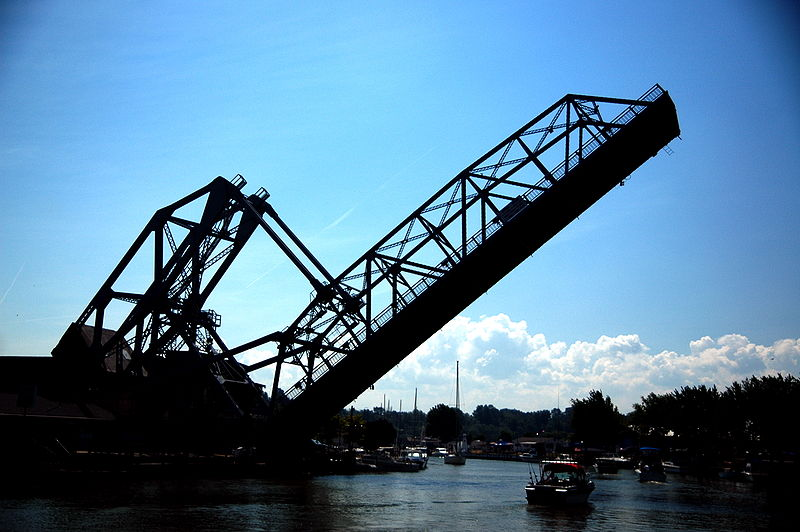
\includegraphics[width=2in]{./LawofSinesGraphics/AshBridge.jpg}}

\smallskip


Assume the bridge casts a shadow directly below itself the entire time it is being raised,\footnote{That is, the sun is directly overhead of the bridge and is shining for an entire two minutes... which never actually happens.} 

\begin{enumerate}

\item  Let $s$ denote the length of the shadow of the bridge on the water.  Show $s = 160 \cos(\theta)$. 
 
\smallskip

\item Assuming  the angle of elevation of the bridge changes at a constant rate, use the related rate law:\footnote{Theorem \ref{relatedratesaroc} in Section  \ref{RelatedRates}} $\frac{\Delta s}{\Delta t} = \frac{\Delta s}{\Delta \theta} \, \frac{\Delta \theta}{\Delta t}$   to help you find the rate of change of the shadow length with respect to time as $\theta$ increases from $30^{\circ}$ to $30.1^{\circ}$.  Remember to give units.


\end{enumerate}

\setcounter{HW}{\value{enumi}}
\end{enumerate}

\begin{enumerate}
\setcounter{enumi}{\value{HW}}

\item Prove that the Law of Sines holds when $\triangle ABC$ is a right triangle.

\item Discuss with your classmates why knowing only the three angles of a triangle is not enough to determine any of the sides.

\item Discuss with your classmates why the Law of Sines cannot be used to find the angles in the triangle when only the three sides are given.  Also discuss what happens if only two sides and the angle between them are given.  (Said another way, explain why the Law of Sines cannot be used in the SSS and SAS cases.)

\item Given $\alpha = 30^{\circ}$ and $b = 10$, choose four different values for $a$ so that 

\begin{enumerate}

\item the information yields no triangle
\item the information yields exactly one right triangle
\item the information yields two distinct triangles
\item the information yields exactly one obtuse triangle

\end{enumerate}

Explain why you cannot choose $a$ in such a way as to have $\alpha = 30^{\circ}$, $b = 10$ and your choice of $a$ yield only one triangle where that unique triangle has three acute angles.

\item Use the cases and diagrams in the proof of the Law of Sines (Theorem \ref{lawofsines}) to prove the area formulas given in Theorem \ref{areaformulasine}.  Why do those formulas yield square units when four quantities are being multiplied together?

\setcounter{HW}{\value{enumi}}

\end{enumerate}

\newpage

\subsection{Answers}

\begin{multicols}{2}

\begin{enumerate}

\item $\begin{array}{lll}
\alpha = 13^{\circ} & \beta = 17^{\circ} & \gamma = 150^{\circ} \\
a = 5 & b \approx 6.50 & c \approx 11.11 \end{array}$

\item $\begin{array}{lll}
\alpha = 73.2^{\circ} & \beta = 54.1^{\circ} & \gamma = 52.7^{\circ} \\
a = 117 & b \approx 99.00 & c \approx 97.22 \end{array}$

\setcounter{HW}{\value{enumi}}

\end{enumerate}

\end{multicols}

\begin{multicols}{2} 

\begin{enumerate}

\setcounter{enumi}{\value{HW}}

\item \begin{tabular}{l}
Information does not \\
produce a triangle \end{tabular}

\item $\begin{array}{lll}
\alpha = 95^{\circ} & \beta = 62^{\circ} & \gamma = 23^{\circ} \\
a = 33.33 & b \approx 29.54 & c \approx 13.07 \end{array}$

\setcounter{HW}{\value{enumi}}

\end{enumerate}

\end{multicols}

\begin{multicols}{2} 

\begin{enumerate}

\setcounter{enumi}{\value{HW}}

\item \begin{tabular}{l}
Information does not \\
produce a triangle \end{tabular}

\item $\begin{array}{lll}
\alpha = 117^{\circ} & \beta \approx 56.3^{\circ} & \gamma \approx 6.7^{\circ} \\
a = 45 & b = 42 & c \approx 5.89 \end{array}$

\setcounter{HW}{\value{enumi}}

\end{enumerate}

\end{multicols}

\begin{multicols}{2} 

\begin{enumerate}

\setcounter{enumi}{\value{HW}}

\item $\begin{array}{lll}
\alpha = 68.7^{\circ} & \beta \approx 76.9^{\circ} & \gamma \approx 34.4^{\circ} \\
a = 88 & b = 92 & c \approx 53.36 \end{array}$

$\begin{array}{lll}
\alpha = 68.7^{\circ} & \beta \approx 103.1^{\circ} & \gamma \approx 8.2^{\circ} \\
a = 88 & b = 92 & c \approx 13.47\end{array}$

\item $\begin{array}{lll}
\alpha = 42^{\circ} & \beta \approx 67.66^{\circ} & \gamma \approx 70.34^{\circ} \\
a = 17 & b = 23.5 & c \approx 23.93 \end{array}$

$\begin{array}{lll}
\alpha = 42^{\circ} & \beta \approx 112.34^{\circ} & \gamma \approx 25.66^{\circ} \\
a = 17 & b = 23.5 & c \approx 11.00 \end{array}$

\setcounter{HW}{\value{enumi}}

\end{enumerate}

\end{multicols}

\begin{multicols}{2} 

\begin{enumerate}

\setcounter{enumi}{\value{HW}}

\item \begin{tabular}{l}
Information does not \\
produce a triangle \end{tabular}

\item $\begin{array}{lll}
\alpha = 30^{\circ} & \beta = 90^{\circ} & \gamma = 60^{\circ} \\
a = 7 & b = 14 & c = 7\sqrt{3} \end{array}$

\setcounter{HW}{\value{enumi}}

\end{enumerate}

\end{multicols}

\begin{multicols}{2} 

\begin{enumerate}

\setcounter{enumi}{\value{HW}}

\item $\begin{array}{lll}
\alpha = 42^{\circ} & \beta \approx 23.78^{\circ} & \gamma \approx 114.22^{\circ} \\
a = 39 & b = 23.5 & c \approx 53.15 \end{array}$

\item $\begin{array}{lll}
\alpha = 53^{\circ} & \beta = 74^{\circ} & \gamma = 53^{\circ} \\
a = 28.01 & b \approx 33.71 & c = 28.01 \end{array}$

\setcounter{HW}{\value{enumi}}

\end{enumerate}

\end{multicols}

\begin{multicols}{2} 

\begin{enumerate}

\setcounter{enumi}{\value{HW}}

\item $\begin{array}{lll}
\alpha = 6^{\circ} & \beta \approx 169.43^{\circ} & \gamma \approx 4.57^{\circ} \\
a = 57 & b = 100 & c \approx 43.45 \end{array}$

$\begin{array}{lll}
\alpha = 6^{\circ} & \beta \approx 10.57^{\circ} & \gamma \approx 163.43^{\circ} \\
a = 57 & b = 100 & c \approx 155.51 \end{array}$

\item $\begin{array}{lll}
\alpha \approx 78.59^{\circ} & \beta \approx 26.81^{\circ} & \gamma = 74.6^{\circ} \\
a = 3.05 & b \approx 1.40 & c = 3 \end{array}$

$\begin{array}{lll}
\alpha \approx 101.41^{\circ} & \beta \approx 3.99^{\circ} & \gamma = 74.6^{\circ} \\
a = 3.05 & b \approx 0.217 & c = 3 \end{array}$

\setcounter{HW}{\value{enumi}}

\end{enumerate}

\end{multicols}

\begin{multicols}{2} 

\begin{enumerate}

\setcounter{enumi}{\value{HW}}

\item $\begin{array}{lll}
\alpha \approx 28.61^{\circ} & \beta = 102^{\circ} & \gamma \approx 49.39^{\circ} \\
a \approx 8.20 & b = 16.75 & c = 13 \end{array}$

\item \begin{tabular}{l}
Information does not \\
produce a triangle \end{tabular}

\setcounter{HW}{\value{enumi}}

\end{enumerate}

\end{multicols}

\begin{multicols}{2} 

\begin{enumerate}

\setcounter{enumi}{\value{HW}}

\item $\begin{array}{lll}
\alpha = 43^{\circ} & \beta = 102^{\circ} & \gamma = 35^{\circ} \\
a \approx 11.68 & b = 16.75 & c \approx 9.82 \end{array}$

\item $\begin{array}{lll}
\alpha = 66.92^{\circ} & \beta = 29.13^{\circ} & \gamma = 83.95^{\circ} \\
a \approx 593.69 & b = 314.15 & c \approx 641.75 \end{array}$

\setcounter{HW}{\value{enumi}}

\end{enumerate}

\end{multicols}

\begin{multicols}{2} 

\begin{enumerate}

\setcounter{enumi}{\value{HW}}

\item \begin{tabular}{l}
Information does not \\
produce a triangle \end{tabular}

\item $\begin{array}{lll}
\alpha = 50^{\circ} & \beta \approx 22.52^{\circ} & \gamma \approx 107.48^{\circ} \\
a = 25 & b = 12.5 & c \approx 31.13 \end{array}$

\setcounter{HW}{\value{enumi}}

\end{enumerate}

\end{multicols}

\begin{enumerate}

\setcounter{enumi}{\value{HW}}

\item The area of the triangle from Exercise \ref{firstlawofsines} is about 8.1 square units.\\
The area of the triangle from Exercise \ref{secondarea} is about 377.1 square units.\\
The area of the triangle from Exercise \ref{lastlawofsines} is about 149 square units.

\item $\arctan\left(\frac{7}{100}\right) \approx 0.699$ radians, which is equivalent to $4.004^{\circ}$
\item About 17\%
\item About 53 feet

\pagebreak

\item \begin{multicols}{4} \begin{enumerate}

\item $\theta = 180^{\circ}$
\item $\theta = 353^{\circ}$
\item $\theta = 84.5^{\circ}$
\item $\theta = 270^{\circ}$

\setcounter{HWindent}{\value{enumii}}

\end{enumerate}

\end{multicols}

\begin{multicols}{4} 

\begin{enumerate}

\setcounter{enumii}{\value{HWindent}}

\item $\theta = 121.25^{\circ}$
\item $\theta = 197^{\circ} 18' 48''$
\item $\theta = 45^{\circ}$
\item $\theta = 225^{\circ}$

\end{enumerate}

\end{multicols}

\item  The Colonel is about 3193 feet from the campfire. \\
Sarge is about 2525 feet to the campfire.

\item The distance from the Muffin Ridge Observatory to Sasquach Point is about 7.12 miles.\\
The distance from Sasquatch Point to the Chupacabra Trailhead is about 2.46 miles.

\item  The SS Bigfoot is about 4.1 miles from the flare. \\
The HMS Sasquatch is about 2.9 miles from the flare.

\item  Jeff is about 371 feet from the nest.

\item  She is about 3.02 miles from the lodge

\item  The boat is about 25.1 miles from the second tower.

\item  The UFO is hovering about 9539 feet above the ground.

\item The gargoyle is about 44 feet from the observer on the upper floor. \\
The gargoyle is about 27 feet from the observer on the lower floor. \\
The gargoyle is about 25 feet from the other building.

\setcounter{HW}{\value{enumi}}
\end{enumerate}

\begin{enumerate}
\setcounter{enumi}{\value{HW}}
\item \begin{enumerate} \addtocounter{enumii}{1}

\item  $\frac{\Delta h}{\Delta t}$ is given as a constant $6 \, \frac{\text{ft}}{\text{s}}$. $\frac{\Delta h}{\Delta \theta} = \frac{h(60.1) - h(60)}{0.1} \approx 0.348 \, \frac{\text{ft}}{\text{degree,  } \,  \circ}$.  

\smallskip

Hence, $\frac{\Delta \theta}{\Delta t} = \frac{ 6 \, \frac{\text{ft}}{\text{s}}   }{ 0.348 \, \frac{\text{ft}}{\text{degree,  } \, \circ}} \approx 17.215 \, \frac{ \text{degree,  } \, \circ}{s}$.  

\smallskip

The angle of elevation is increasing at an average rate of $17.215$ degrees  per second.  

\smallskip

\textbf{WARNING:} For (good) reasons you'll explore more deeply in Calculus, you'll usually stick with radians when the Calculus version of this problem rolls around \ldots  

\end{enumerate}


\item  \begin{enumerate} \addtocounter{enumii}{1}

\item   $\frac{\Delta s}{\Delta \theta} = \frac{s(30.1) - s(30)}{0.1} \approx -1.398 \, \frac{\text{ft}}{\text{degree} \,  \circ}$.  

\smallskip

We are told to assume $\frac{\Delta \theta }{\Delta t}$ is a constant, so $\frac{\Delta s}{\Delta t} = \frac{45^{\circ}}{2 \, \text{minutes}} = 22.5 \, \frac{\text{degree,  } \, \circ}{\text{min}}$.

\smallskip

We get:  $\frac{\Delta s}{\Delta t} = \frac{\Delta s}{\Delta \theta} \, \frac{\Delta \theta }{\Delta t} \approx \left(-1.398 \, \frac{\text{ft}}{\text{degree,  } \,  \circ} \right) \left(  22.5 \, \frac{\text{degree,  } \, \circ}{\text{min}} \right) \approx -31.436 \, \frac{\text{ft}}{\text{min}}$.

\smallskip

This means the shadow is receding at a rate of approximately 31.436 feet per minute.

\smallskip

\textbf{WARNING:} For (good) reasons you'll explore more deeply in Calculus, you'll usually stick with radians when the Calculus version of this problem rolls around \ldots  

\end{enumerate}


\setcounter{HW}{\value{enumi}}
\end{enumerate}




\end{document}


\closegraphsfile

\end{document}


\newpage

\section{The Law of Cosines}

\documentclass{ximera}

\begin{document}
	\author{Stitz-Zeager}
	\xmtitle{TITLE}


\mfpicnumber{1}

\opengraphsfile{TheLawofCosines}

\setcounter{footnote}{0}

\label{TheLawofCosines}


In Section \ref{TheLawofSines}, we developed the Law of Sines (Theorem \ref{lawofsines}) to enable us to solve triangles in the `Angle-Angle-Side' (AAS), the `Angle-Side-Angle' (ASA) and the ambiguous `Angle-Side-Side' (ASS) cases.  

\smallskip

In this section, we develop the Law of Cosines which handles solving triangles in the \index{Side-Angle-Side triangle} `Side-Angle-Side' (SAS) and \index{Side-Side-Side triangle} `Side-Side-Side' (SSS) cases.\footnote{Here, `Side-Angle-Side' means that we are given two sides and the `included' angle - that is, the given angle is adjacent to both of the given sides.}  We state and prove the theorem below.

\smallskip

\colorbox{ResultColor}{\bbm

\begin{theorem} \label{lawofcosines} \index{Law of Cosines} \textbf{Law of Cosines:}   Given a triangle with angle-side opposite pairs $(\alpha, a)$, $(\beta, b)$ and $(\gamma, c)$, the following equations hold

\[ a^2 = b^2 + c^2 - 2bc \cos(\alpha) \qquad  b^2 = a^2 + c^2 - 2ac \cos(\beta)  \qquad   c^2 = a^2 + b^2 - 2ab \cos(\gamma)  \]

or, solving for the cosine in each equation, we have
 
\[ \cos(\alpha) = \dfrac{b^2+c^2 - a^2}{2bc} \qquad \cos(\beta) = \dfrac{a^2+c^2 - b^2}{2ac} \qquad \cos(\gamma) = \dfrac{a^2+b^2 - c^2}{2ab} \]


\smallskip

\end{theorem}

\ebm}

\smallskip

To prove the theorem, we consider a generic triangle with the vertex of angle $\alpha$ at the origin with side $b$ positioned along the positive $x$-axis as sketched in the diagram below.

\begin{center}

\begin{mfpic}[15]{-10}{10}{-9}{9}
\axes
\drawcolor[gray]{0.7}
\circle{(0,0),7.07}
\drawcolor{black}
\tlabel[cc](7,2.5){$a$}
\tlabel[cc](4,-1){$b$}
\tlabel[cc](2,2.75){$c$}
\tlabel[cc](1.75,0.75){$\alpha$}
\tlabel[cc](0,-0.75){$A=(0,0)$}
\tlabel[cc](8.5,-0.75){$C=(b,0)$}
\arrow \reverse \arrow \parafcn{5, 40, 5}{1.5*dir(t)}
\point[4pt]{(0,0), (8,0), (5,5)}
\gclear \tlabelrect[cc](5,5.75){$B=(c \cos(\alpha), c \sin(\alpha))$}
\penwd{1.25pt}
\polyline{(0,0), (8,0), (5,5), (0,0)}
\end{mfpic}

\end{center}

From this set-up, we immediately find that the coordinates of $A$ and $C$ are $A(0,0)$ and $C(b,0)$.  From Theorem \ref{cosinesinecircle}, we know that since the point $B(x,y)$ lies on a circle of radius $c$, the coordinates of $B$ are $B(x,y) = B(c \cos(\alpha), c \sin(\alpha))$.  (This would be true even if $\alpha$ were an obtuse or right angle so although we have drawn the case when $\alpha$ is acute, the following computations hold for any angle $\alpha$ drawn in standard position where $0 < \alpha < 180^{\circ}$.) 

\smallskip

 We note that the distance between the points $B$ and $C$ is none other than the length of side $a$.  Using the distance formula, Equation \ref{distanceformula}, we get

\[\begin{array}{rclr}
a & = & \sqrt{(c \cos(\alpha) - b)^{2} + (c \sin(\alpha) - 0)^2} & \\ [3pt]
a^{2} & = & \left(\sqrt{(c \cos(\alpha) - b)^{2} + c^2 \sin^2(\alpha)}\right)^2 & \\  [3pt]
a^2 & = &  (c \cos(\alpha) - b)^{2} + c^2 \sin^2(\alpha) & \\  [3pt]
a^2 & = & c^2 \cos^2(\alpha) - 2bc \cos(\alpha) + b^2 + c^2 \sin^2(\alpha) & \\  [3pt]
a^2 & = & c^2\left(\cos^2(\alpha) + \sin^2(\alpha)\right) + b^2 - 2bc \cos(\alpha) & \\  [3pt]
a^2 & = & c^2(1) + b^2 - 2bc \cos(\alpha) & \text{Since $\cos^2(\alpha) + \sin^2(\alpha) = 1$}\\  [3pt]
a^2 & = & c^2 + b^2 - 2bc \cos(\alpha) & \\
\end{array} \]

The remaining formulas given in Theorem \ref{lawofcosines} can be shown by simply reorienting the triangle to place a different vertex at the origin.  We leave these details to the reader.  

\smallskip

What's important about $a$ and $\alpha$ in the above proof is that $(\alpha,a)$ is an angle-side opposite pair and $b$ and $c$ are the sides adjacent to $\alpha$ -- the same can be said of any other angle-side opposite pair in the triangle.   

\smallskip

Notice that the proof of the Law of Cosines relies on the distance formula which has its roots in the Pythagorean Theorem.  That being said, the Law of Cosines can be thought of as a \textit{generalization} of the Pythagorean Theorem. 

\smallskip

Indeed, in a triangle in which $\gamma = 90^{\circ}$, (i.e., a right triangle) then $\cos(\gamma) = \cos\left(90^{\circ}\right) = 0$  and we get the familiar relationship  $c^2 = a^2 + b^2$.  What this means is that in the larger mathematical sense, the Law of Cosines and the Pythagorean Theorem amount to pretty much the same thing.\footnote{This shouldn't come as too much of a shock.  All of the theorems in Trigonometry can ultimately be traced back to the definition of the circular functions along with the distance formula and hence, the Pythagorean Theorem.}

\begin{example}  \label{locex}  Solve the following triangles.  Give exact answers and decimal approximations (rounded to hundredths) and sketch the triangle.

\begin{multicols}{2}

\begin{enumerate}

\item  \label{locsas} $\beta = 50^{\circ}$, $a = 7$ units, $c=2$ units

\item  \label{locsss} $a=4$ units, $b=7$ units, $c = 5$ units

\end{enumerate}

\end{multicols}

{\bf Solution.}

\begin{enumerate}

\item  We are given the lengths of two sides, $a=7$ and $c = 2$, and the measure of the included angle, $\beta = 50^{\circ}$.  With no angle-side opposite pair to use for the Law of Sines, we apply  the Law of Cosines.  We get  $b^2 = 7^2 + 2^2 - 2(7)(2)\cos\left(50^{\circ}\right)$ which yields $b = \sqrt{53-28\cos\left(50^{\circ}\right)} \approx 5.92$ units.  
\smallskip

In order to determine the measures of the remaining angles $\alpha$ and $\gamma$, we are forced to used the derived value for $b$.  There are two ways to proceed at this point.  We could use the Law of Cosines again, or, since  we have the angle-side opposite pair $(\beta, b)$ we could use the Law of Sines. 

\smallskip

The advantage to using the Law of Cosines over the Law of Sines in cases like this is that unlike the sine function, the cosine function distinguishes between acute and obtuse angles.  The cosine of an acute is positive, whereas the cosine of an obtuse angle is negative.  Since the sine of both acute and obtuse angles are positive, the sine of an angle alone is not enough to determine if the angle in question is acute or obtuse.  

\smallskip

Since both authors of the textbook prefer the Law of Cosines, we proceed with this method first.  When using the Law of Cosines, it's always best to find the measure of the largest unknown angle first, since this will give us the obtuse angle of the triangle if there is one.  

\smallskip

Since the largest angle is opposite the longest side, we choose to find $\alpha$ first. To that end, we use the formula $\cos(\alpha) = \frac{b^2+c^2-a^2}{2bc}$ and substitute $a = 7$, $b =  \sqrt{53-28\cos\left(50^{\circ}\right)}$ and $c = 2$. We get\footnote{after simplifying \ldots} \[\cos(\alpha) = \frac{2-7\cos\left(50^{\circ}\right)}{\sqrt{53-28\cos\left(50^{\circ}\right)}}\]  

\smallskip

Since $\alpha$ is an angle in a triangle, we know the radian measure of $\alpha$ must lie between $0$ and $\pi$ radians.  This matches the range of the arccosine function, so we have \[\alpha = \arccos\left(\frac{2-7\cos\left(50^{\circ}\right)}{\sqrt{53-28\cos\left(50^{\circ} \right)}}\right) \, \text{radians} \, \approx  114.99^{\circ}\] At this point, we could find $\gamma$ using $\gamma = 180^{\circ} - \alpha - \beta \approx 180^{\circ} - 114.99^{\circ} - 50^{\circ} = 15.01^{\circ}$, that is if we trust our approximation for $\alpha$. 

\smallskip

To minimize propagation of error (and obtain an \textit{exact} answer for $\gamma$), however, we could use the Law of Cosines again.\footnote{Your instructor will let you know which procedure to use. It all boils down to how much you trust your calculator.} From $\cos(\gamma) = \frac{a^2+b^2-c^2}{2ab}$ with $a = 7$, $b = \sqrt{53-28\cos\left(50^{\circ} \right)}$ and $c=2$, we get  $\gamma = \arccos\left(\frac{7-2 \cos\left(50^{\circ}\right)}{\sqrt{53-28\cos\left(50^{\circ} \right)}} \right)$ radians $\approx 15.01^{\circ}$.  We sketch the triangle below.

\begin{center}


\begin{mfpic}[30]{-2}{6}{0}{2}
\tlabel[cc](2,1.25){\scriptsize $a = 7$}
\tlabel[cc](2,-0.25){\scriptsize  $b \approx 5.92$}
\tlabel[cc](-1,0.5){\scriptsize  $c =2$}
\tlabel[cc](1,0.5){\scriptsize  $\alpha \approx 114.99^{\circ}$}
\tlabel[cc](3,0.25){\scriptsize $\gamma \approx 15.01^{\circ}$}
\tlabel[cc](0.1,1.1){\scriptsize  $\beta = 50^{\circ}$}
\arrow \reverse \arrow \parafcn{5, 115, 5}{0.5*dir(t)}
\arrow \reverse \arrow \shiftpath{(5.72,0)}  \parafcn{168, 178, 5}{2*dir(t)}
\arrow \reverse \arrow \shiftpath{(-1.04,1.81)}  \parafcn{305, 335, 5}{0.75*dir(t)}
\penwd{1.25pt}
\polyline{(0,0), (5.72,0), (-1.04,1.81), (0,0)}
\end{mfpic}

\end{center}

As we mentioned earlier, once we've determined $b$ it is possible to use the Law of Sines to find the remaining angles.  Here, however, we must proceed with caution as we are in the ambiguous (ASS) case.  Here it  is advisable to first find the \textit{smallest} of the unknown angles, since we are guaranteed it will be acute.\footnote{There can only be one \textit{obtuse} angle in the triangle, and if there is one, it must be the largest.} 

\smallskip

In this case, we would find $\gamma$ since the side opposite $\gamma$ is smaller than the side opposite the other unknown angle, $\alpha$.   Using the angle-side opposite pair $(\beta, b)$, we get $\frac{\sin(\gamma)}{2} = \frac{\sin(50^{\circ})}{ \sqrt{53-28\cos\left(50^{\circ}\right)}}$.  The usual calculations produces $\gamma \approx  15.01^{\circ}$ and $\alpha = 180^{\circ} - \beta - \gamma \approx 180^{\circ} - 50^{\circ} - 15.01^{\circ} = 114.99^{\circ}$.


\item  Since all three sides and no angles are given, we are forced to use the Law of Cosines.  Following our discussion in the previous problem, we find $\beta$ first, since it is opposite the longest side, $b$. We get $\cos(\beta) = \frac{a^2+c^2-b^2}{2ac} = -\frac{1}{5}$, so  $\beta = \arccos\left(-\frac{1}{5}\right)$ radians $\approx 101.54^{\circ}$.  

\smallskip

Now that we have obtained an angle-side opposite pair $(\beta, b)$, we could proceed using the Law of Sines.  The Law of Cosines, however, offers us a rare opportunity to find the remaining angles using \textit{only} the data given to us in the statement of the problem.

\smallskip

 Using the Law of Cosines, we get  $\gamma = \arccos\left(\frac{5}{7}\right)$ radians $\approx 44.42^{\circ}$ and  $\alpha = \arccos\left(\frac{29}{35}\right)$ radians $\approx 34.05^{\circ}$.  We sketch this triangle below.

\begin{center}

\begin{mfpic}[30]{0}{7}{0}{2}
\tlabel[cc](6.25,1.5){\scriptsize $a = 4$}
\tlabel[cc](1.5,1.5){\scriptsize  $c = 5$}
\tlabel[cc](2,0.35){\scriptsize $\alpha \approx 34.05^{\circ}$}
\tlabel[cc](4,2){\scriptsize $\beta \approx 101.54^{\circ}$}
\tlabel[cc](5,0.35){\scriptsize $\gamma \approx 44.42^{\circ}$}
\tlabel[cc](3.5,-0.25){\scriptsize $b = 7$}
\arrow \reverse \arrow \parafcn{5, 30, 5}{1.25*dir(t)}
\arrow \reverse \arrow  \shiftpath{(4.14,2.8)}  \parafcn{220, 310, 5}{0.5*dir(t)}
\arrow \reverse \arrow  \shiftpath{(7,0)}  \parafcn{140, 175, 5}{1.25*dir(t)}
\penwd{1.25pt}
\polyline{(0,0), (4.14,2.8), (7,0),(0,0)}
\end{mfpic}

\end{center}

\end{enumerate}
\vspace{-.5in} \qed
\end{example}

We note that, depending on how many decimal places are carried through successive calculations, and depending on which approach is used to solve the problem, the approximate answers you obtain may differ slightly from those the authors obtain in the Examples and the Exercises.  

\smallskip

A great example of this is number   \ref{locsss} in  Example \ref{locex}, where the \textit{approximate} values we record for the measures of the angles sum to $180.01^{\circ}$, which is geometrically impossible. 
\smallskip

\begin{example}  \label{locapplication}  A researcher wishes to determine the width of a vernal pond as drawn below. From a point $P$, he finds the distance to the eastern-most point of the pond to be $950$ feet, while the distance to the western-most point of the pond from $P$ is $1000$ feet. If the angle between the two lines of sight is $60^{\circ}$, find the width of the pond.

\begin{center}

\begin{mfpic}[15]{-5}{5}{-5}{5}
\fillcolor[gray]{0.7}
\gfill \cyclic[1.25]{(-5,-3), (-3,0), (-1,2), (0,0), (1,1), (3,2), (4,4), (5,4.75), (3,-2), (0,-3), (-3,-2),  (-5,-3)}
\plotsymbol[5pt]{Asterisk}{(-5,-3),(5,5)}
\dashed \polyline{(-5,-3), (5,5)}
\dashed \polyline{(-5,-3), (4.25,-5), (5,5)}
\tlabel[cc](-0.5,-4.75){$950$ feet}
\tlabel(4.75,0){$1000$ feet}
\arrow \reverse \arrow \shiftpath{(4.25,-5)}  \parafcn{100, 160, 5}{1.5*dir(t)}
\tlabel[cc](3,-3){$60^{\circ}$}
\point[3pt]{(4.25,-5)}
\tlabel[cc](4.25,-5.5){$P$}
\end{mfpic}

\end{center}

{\bf Solution.}  We are given the lengths of two sides and the measure of an included angle, so we may apply the Law of Cosines to find the length of the missing side opposite the given angle. 

\smallskip

 Calling this length $w$ (for \textit{width}), we get  $w^2 = 950^2 + 1000^2 - 2(950)(1000)\cos\left(60^{\circ}\right) = 952500$ from which we get $w = \sqrt{952500} \approx 976$ feet.  \qed

\end{example}

In Section \ref{TheLawofSines}, we used the proof of the Law of Sines to develop Theorem \ref{areaformulasine} as an alternate formula for the area enclosed by a triangle.  In this section, we use the Law of Cosines to derive another such formula,  the so-called Heron's Formula.\footnote{Or \href{http://bit.ly/2rwhWoJ}{`\underline{Hero's Formula}.'}}

\smallskip

\colorbox{ResultColor}{\bbm 

\begin{theorem}  \label{HeronsFormula}  \index{Heron's Formula} \textbf{Heron's Formula:} Suppose $a$, $b$ and $c$ denote the lengths of the three sides of a triangle.  Let $s$ be the semiperimeter of the triangle, that is, let $s = \frac{1}{2}(a + b + c)$.  Then the area $A$ enclosed by the triangle is given by

\[ A = \sqrt{s (s-a) (s-b) (s-c)}\]

\smallskip

\end{theorem}

\ebm}

\smallskip

We prove Theorem \ref{HeronsFormula} using Theorem \ref{areaformulasine}.  Using the convention that the angle $\gamma$ is opposite the side $c$,  we have $A = \frac{1}{2} ab \sin(\gamma)$ from Theorem \ref{areaformulasine}. 

\smallskip

In order to simplify computations, we start by manipulating the expression for $A^2$.

\[ \begin{array}{rclr} 

A^2 & = & \left(\dfrac{1}{2} ab \sin(\gamma)\right)^2 &\\[10pt] 
    & =  &  \dfrac{1}{4} a^2 b^2 \sin^{2}(\gamma) & \\[10pt]
    & = & \dfrac{a^2b^2}{4} \left(1 - \cos^{2}(\gamma)\right) & \text{since $\sin^2(\gamma) = 1 - \cos^{2}(\gamma)$.} \\ \end{array}\]

The Law of Cosines tells us $\cos(\gamma) = \frac{a^2 + b^2 - c^2}{2ab}$, so substituting this into our equation for $A^2$ gives

\[ \begin{array}{rclr}

A^2 & = &  \dfrac{a^2b^2}{4} \left(1 - \cos^{2}(\gamma)\right) 	& \text{\hphantom{perfect square trinomials.}}\\[10pt]

    & = & \dfrac{a^2b^2}{4} \left[1 - \left( \dfrac{a^2 + b^2 - c^2}{2ab} \right)^2\right] &  \\ [10pt]
    
	 	& = & \dfrac{a^2b^2}{4} \left[1 - \dfrac{\left(a^2 + b^2 - c^2\right)^2}{4a^2b^2} \right] &  \\ [10pt]  
		
		& = & \dfrac{a^2b^2}{4} \left[\dfrac{4a^2 b^2  - \left(a^2 + b^2 - c^2\right)^2}{4a^2b^2} \right] &   \\ [10pt]
		
		& = & \dfrac{4a^2 b^2  - \left(a^2 + b^2 - c^2\right)^2}{16}  &  \\  \end{array} \]
	
	
Recognizing $4a^2 b^2$ as a perfect square, $4a^2 b^2 = (2ab)^2$, we can factor the resulting difference of squares:
		
\[ \begin{array}{rclr}
	 
	 	
	A^2 	& = & \dfrac{(2ab)^2  - \left(a^2 + b^2 - c^2\right)^2}{16}  &  \\ [10pt]
	 	
	 		& = & \dfrac{\left( 2ab - \left[a^2+b^2 - c^2\right]\right)  \left( 2ab + \left[a^2+b^2 - c^2\right]\right)}{16}  & \text{difference of squares.} \\ [10pt]
	 	 	& = & \dfrac{\left(c^2 - a^2 + 2ab - b^2 \right)\left( a^2 + 2ab + b^2- c^2\right)}{16}  &  \\ [10pt]
	 	\end{array} \]
		
Next, we regroup $c^2 - a^2 + 2ab - b^2 = c^2 - \left[a^2 - 2ab + b^2\right]$ and  $a^2 + 2ab + b^2- c^2 = \left[a^2 + 2ab + b^2\right]- c^2$.  Recognizing $a^2 - 2ab + b^2 = (a-b)^2$ and $a^2 + 2ab + b^2 = (a+b)^2$, we continue factoring:
	 	
\[ \begin{array}{rclr}

A^2	& = & \dfrac{\left(c^2 - \left[a^2 - 2ab + b^2\right] \right)  \left( \left[a^2 + 2ab + b^2\right]- c^2\right)}{16}  &  \\ [10pt]

	 	& = & \dfrac{\left(c^2 - (a-b)^2 \right)  \left( (a+b)^2- c^2\right)}{16}  &  \text{perfect square trinomials.}\\ [10pt]
	 	
	 	& = & \dfrac{ (c-(a-b))(c+(a-b))((a+b) -c)((a+b)+c)}{16}  &  \text{difference of squares.} \\ [10pt]
	 			 
	 	& = & \dfrac{ (b+c-a)(a+c-b)(a+b-c)(a+b+c)}{16}  &  \\ [10pt]	 	
	 	
	  & = & \dfrac{(b+c-a)}{2} \cdot \dfrac{(a+c-b)}{2} \cdot \dfrac{(a+b-c)}{2} \cdot \dfrac{(a+b+c)}{2}  &  \\ [10pt]	 
	 		
\end{array} \]

At this stage, we recognize the last factor as the semiperimeter, $s = \frac{1}{2}(a+b+c) = \frac{a+b+c}{2}$.  To complete the proof, we note that

\[ (s - a) = \dfrac{a+b+c}{2} - a = \dfrac{a+b+c-2a}{2} = \dfrac{b+c-a}{2} \]  
			
Similarly, we find $(s-b) = \frac{a+c-b}{2}$ and $(s-c) = \frac{a+b-c}{2}$.  Hence, we get

\[ \begin{array}{rclr}

A^2 & = & \dfrac{(b+c-a)}{2} \cdot \dfrac{(a+c-b)}{2} \cdot \dfrac{(a+b-c)}{2} \cdot \dfrac{(a+b+c)}{2}  &  \\ [10pt]	 
	 	
	 	& = & (s-a) (s-b) (s-c) s  &  \\ [10pt]	 	
	 	
\end{array} \]

so that  $A = \sqrt{s(s-a)(s-b)(s-c)}$ as required. 

\smallskip

We close with an example of Heron's Formula.

\begin{example} \label{heronex}  Find the area enclosed of the triangle in Example \ref{locex} number \ref{locsss}.

\medskip

{\bf Solution.}  We are given $a = 4$, $b=7$ and $c = 5$.  Using these values, we find $s = \frac{1}{2}(4+7+5) = 8$, $(s - a) = 8 - 4 = 4$, $(s-b) = 8-7 =1$ and $(s-c) = 8-5=3$. 

\smallskip

Per Heron's Formula,  $A = \sqrt{s(s-a)(s-b)(s-c)} = \sqrt{(8)(4)(1)(3)} = \sqrt{96} = 4\sqrt{6} \approx 9.80$ square units. \qed

\end{example}

\newpage

\subsection{Exercises}

%% SKIPPED %% \documentclass{ximera}

\begin{document}
	\author{Stitz-Zeager}
	\xmtitle{TITLE}


In Exercises \ref{firstlawofcosines} - \ref{lastlawofcosines}, use the Law of Cosines to find the remaining side(s) and angle(s) if possible.

\begin{multicols}{2}

\begin{enumerate}

\item $a = 7, \; b = 12, \; \gamma = 59.3^{\circ}$ \label{firstlawofcosines}
\item $\alpha = 104^{\circ}, \; b = 25, \; c  = 37$

\setcounter{HW}{\value{enumi}}

\end{enumerate}

\end{multicols}

\begin{multicols}{2} 

\begin{enumerate}

\setcounter{enumi}{\value{HW}}

\item $a = 153, \; \beta = 8.2^{\circ}, \; c = 153$
\item $a = 3, \; b = 4, \; \gamma = 90^{\circ}$

\setcounter{HW}{\value{enumi}}

\end{enumerate}

\end{multicols}

\begin{multicols}{2} 

\begin{enumerate}

\setcounter{enumi}{\value{HW}}

\item $\alpha = 120^{\circ}, \; b = 3, \; c = 4$
\item $a = 7, \; b = 10, \; c = 13$ \label{firstherons}

\setcounter{HW}{\value{enumi}}

\end{enumerate}

\end{multicols}

\begin{multicols}{2} 

\begin{enumerate}

\setcounter{enumi}{\value{HW}}

\item $a = 1, \; b = 2, \; c = 5$
\item $a = 300, \; b = 302, \; c = 48$ \label{secondherons}

\setcounter{HW}{\value{enumi}}

\end{enumerate}

\end{multicols}

\begin{multicols}{2} 

\begin{enumerate}

\setcounter{enumi}{\value{HW}}

\item $a = 5, \; b = 5, \; c = 5$
\item $a = 5, \; b = 12,; c = 13$ \label{thirdherons} \label{lastlawofcosines}

\setcounter{HW}{\value{enumi}}

\end{enumerate}

\end{multicols}

In Exercises \ref{anylawfirst} - \ref{anylawlast}, use any method to solve for the remaining side(s) and angle(s), if possible.

\begin{multicols}{2}

\begin{enumerate}

\setcounter{enumi}{\value{HW}}

\item $a = 18, \; \alpha = 63^{\circ}, \; b = 20$ \label{ambigfirst} \label{anylawfirst}
\item $a = 37, \; b = 45, \; c = 26$

\setcounter{HW}{\value{enumi}}

\end{enumerate}

\end{multicols}

\begin{multicols}{2} 

\begin{enumerate}

\setcounter{enumi}{\value{HW}}

\item $a = 16, \; \alpha = 63^{\circ}, \; b = 20$ \label{ambigsecond}
\item $a = 22, \; \alpha = 63^{\circ}, \; b = 20$ \label{ambigthird}

\setcounter{HW}{\value{enumi}}

\end{enumerate}

\end{multicols}

\begin{multicols}{2} 

\begin{enumerate}

\setcounter{enumi}{\value{HW}}

\item $\alpha = 42^{\circ}, \; b = 117, \; c = 88$
\item $\beta = 7^{\circ}, \; \gamma = 170^{\circ}, \; c = 98.6$ \label{anylawlast}

\setcounter{HW}{\value{enumi}}

\end{enumerate}

\end{multicols}

\begin{enumerate}

\setcounter{enumi}{\value{HW}}

\item Find the area of the triangles given in Exercises \ref{firstherons}, \ref{secondherons} and \ref{thirdherons} above.

\item The hour hand on my antique Seth Thomas schoolhouse clock in 4 inches long and the minute hand is 5.5 inches long.  Find the distance between the ends of the hands when the clock reads four o'clock.  Round your answer to the nearest hundredth of an inch.

\item A geologist wants to measure the diameter of an impact crater.   From her camp, it is 4 miles to the northern-most point of the crater and 2 miles to the southern-most point.  If the angle between the two lines of sight is $117^{\circ}$, what is the diameter of the crater?  Round your answer to the nearest hundredth of a mile.

\item From the Pedimaxus International Airport a tour helicopter can fly to Cliffs of Insanity Point by following a bearing of N$8.2^{\circ}$E for 192 miles and it can fly to Bigfoot Falls by following a bearing of S$68.5^{\circ}$E for 207 miles.\footnote{Please refer to Section \ref{bearings} for an introduction to bearings.}  Find the distance between Cliffs of Insanity Point and Bigfoot Falls.  Round your answer to the nearest mile.  \label{lofcosinesbearingexercise}

\item Cliffs of Insanity Point and Bigfoot Falls from Exericse \ref{lofcosinesbearingexercise} above both lie on a straight stretch of the Great Sasquatch Canyon.  What bearing would the tour helicopter need to follow to go directly from Bigfoot Falls to Cliffs of Insanity Point?  Round your angle to the nearest tenth of a degree.

\item  A naturalist sets off on a hike from a lodge on a bearing of S$80^{\circ}$W.  After 1.5 miles, she changes her bearing to S$17^{\circ}$W and continues hiking for 3 miles.  Find her distance from the lodge at this point.  Round your answer to the nearest hundredth of a mile.  What bearing should she follow to return to the lodge?  Round your angle to the nearest degree.

\item The HMS Sasquatch leaves port on a bearing of N$23^{\circ}$E and travels for 5 miles.  It then changes course and follows a heading of S$41^{\circ}$E for 2 miles.  How far is it from port? Round your answer to the nearest hundredth of a mile. What is its bearing to port?  Round your angle to the nearest degree.

\item  The SS Bigfoot leaves a harbor bound for Nessie Island which is 300 miles away at a bearing of N$32^{\circ}$E.  A storm moves in and after 100 miles, the captain of the Bigfoot finds he has drifted off course.  If his bearing to the harbor is now S$70^{\circ}$W, how far is the SS Bigfoot from Nessie Island?  Round your answer to the nearest hundredth of a mile.  What course should the captain set to head to the island?  Round your angle to the nearest tenth of a degree.

\item From a point 300 feet above level ground in a firetower, a ranger spots two fires in the Yeti National Forest.  The angle of depression\footnote{See Exercise \ref{angleofdepression} in Section \ref{AppRightTrig} for the definition of this angle.} made by the line of sight from the ranger to the first fire is $2.5^{\circ}$ and the angle of depression made by line of sight from the ranger to the second fire is $1.3^{\circ}$.  The angle formed by the two lines of sight is $117^{\circ}$.  Find the distance between the two fires.  Round your answer to the nearest foot. 
\begin{center}
\begin{mfpic}[15]{-5}{5}{-5}{5}
\plotsymbol[5pt]{Asterisk}{(-4.33,2.5),(2.6, 1.5)}
\tlabel[cc](0,-0.5){firetower}
\tlabel[cc](4.5,1.5){fire}
\tlabel[cc](-5.5, 2.5){fire}
\arrow \reverse \arrow \parafcn{35, 145, 5}{1.5*dir(t)}
\tlabel[cc](0,2){$117^{\circ}$}
\point[4pt]{(0,0)}
\dashed \polyline{(0,0), (-4.33,2.5)}
\dashed \polyline{(0,0), (2.6, 1.5)}
\end{mfpic}


\end{center}

HINT: In order to use the $117^{\circ}$ angle between the lines of sight, you will first need to use right angle Trigonometry to find the lengths of the lines of sight.  This will give you a Side-Angle-Side case in which to apply the Law of Cosines.



\item If you apply the Law of Cosines to the ambiguous Angle-Side-Side (ASS) case, the result is a quadratic equation whose variable is that of the missing side. If the equation has no positive real zeros then the information given does not yield a triangle.  If the equation has only one positive real zero then exactly one triangle is formed and if the equation has two distinct positive real zeros then two distinct triangles are formed.  Apply the Law of Cosines to Exercises \ref{ambigfirst}, \ref{ambigsecond} and \ref{ambigthird} above in order to demonstrate this result.  

\item Discuss with your classmates why Heron's Formula yields an area in square units even though four lengths are being multiplied together.

\end{enumerate}

\newpage

\subsection{Answers}

\begin{multicols}{2}

\begin{enumerate}

\item $\begin{array}{lll}
\alpha \approx 35.54^{\circ} & \beta \approx 85.16^{\circ} & \gamma = 59.3^{\circ} \\
a = 7 & b = 12 & c \approx 10.36 \end{array}$

\item $\begin{array}{lll}
\alpha = 104^{\circ} & \beta \approx 29.40^{\circ} & \gamma \approx 46.60^{\circ} \\
a \approx 49.41 & b = 25 & c = 37 \end{array}$

\setcounter{HW}{\value{enumi}}

\end{enumerate}

\end{multicols}

\begin{multicols}{2} 

\begin{enumerate}

\setcounter{enumi}{\value{HW}}

\item $\begin{array}{lll}
\alpha \approx 85.90^{\circ} & \beta = 8.2^{\circ} & \gamma \approx 85.90^{\circ} \\
a = 153 & b \approx 21.88 & c = 153 \end{array}$

\item $\begin{array}{lll}
\alpha \approx 36.87^{\circ} & \beta \approx 53.13^{\circ} & \gamma = 90^{\circ} \\
a = 3 & b = 4 & c = 5 \end{array}$

\setcounter{HW}{\value{enumi}}

\end{enumerate}

\end{multicols}

\begin{multicols}{2} 

\begin{enumerate}

\setcounter{enumi}{\value{HW}}

\item $\begin{array}{lll}
\alpha = 120^{\circ} & \beta \approx 25.28^{\circ} & \gamma \approx 34.72^{\circ} \\
a = \sqrt{37} & b = 3 & c = 4 \end{array}$

\item $\begin{array}{lll}
\alpha \approx 32.31^{\circ} & \beta \approx 49.58^{\circ} & \gamma \approx 98.21^{\circ} \\
a = 7 & b = 10 & c = 13 \end{array}$

\setcounter{HW}{\value{enumi}}

\end{enumerate}

\end{multicols}

\begin{multicols}{2} 

\begin{enumerate}

\setcounter{enumi}{\value{HW}}

\item \begin{tabular}{l}
Information does not \\
produce a triangle \end{tabular}

\item $\begin{array}{lll}
\alpha \approx 83.05^{\circ} & \beta \approx 87.81^{\circ} & \gamma \approx 9.14^{\circ} \\
a = 300 & b = 302 & c = 48 \end{array}$

\setcounter{HW}{\value{enumi}}

\end{enumerate}

\end{multicols}

\begin{multicols}{2} 

\begin{enumerate}

\setcounter{enumi}{\value{HW}}

\item $\begin{array}{lll}
\alpha = 60^{\circ} & \beta = 60^{\circ} & \gamma = 60^{\circ} \\
a = 5 & b = 5 & c = 5 \end{array}$

\item $\begin{array}{lll}
\alpha \approx 22.62^{\circ} & \beta \approx 67.38^{\circ} & \gamma = 90^{\circ} \\
a = 5 & b = 12 & c = 13 \end{array}$

\setcounter{HW}{\value{enumi}}

\end{enumerate}

\end{multicols}

\begin{multicols}{2}

\begin{enumerate}

\setcounter{enumi}{\value{HW}}

\item $\begin{array}{lll}
\alpha = 63^{\circ} & \beta \approx 98.11^{\circ} & \gamma \approx 18.89^{\circ} \\
a = 18 & b = 20 & c \approx 6.54 \end{array}$

$\begin{array}{lll}
\alpha = 63^{\circ} & \beta \approx 81.89^{\circ} & \gamma \approx 35.11^{\circ} \\
a = 18 & b = 20 & c \approx 11.62 \end{array}$

\item $\begin{array}{lll}
\alpha \approx 55.30^{\circ} & \beta \approx 89.40^{\circ} & \gamma \approx 35.30^{\circ} \\
a = 37 & b = 45 & c = 26 \end{array}$

\setcounter{HW}{\value{enumi}}

\end{enumerate}

\end{multicols}

\begin{multicols}{2} 

\begin{enumerate}

\setcounter{enumi}{\value{HW}}

\item \begin{tabular}{l}
Information does not \\
produce a triangle \end{tabular}

\item $\begin{array}{lll}
\alpha = 63^{\circ} & \beta \approx 54.1^{\circ} & \gamma \approx 62.9^{\circ} \\
a = 22 & b = 20 & c \approx 21.98 \end{array}$

\setcounter{HW}{\value{enumi}}

\end{enumerate}

\end{multicols}

\begin{multicols}{2} 

\begin{enumerate}

\setcounter{enumi}{\value{HW}}

\item $\begin{array}{lll}
\alpha = 42^{\circ} & \beta \approx 89.23^{\circ} & \gamma \approx 48.77^{\circ} \\
a \approx 78.30 & b = 117 & c = 88 \end{array}$

\item $\begin{array}{lll}
\alpha \approx 3^{\circ} & \beta = 7^{\circ} & \gamma = 170^{\circ} \\
a \approx 29.72 & b \approx 69.2 & c = 98.6 \end{array}$

\setcounter{HW}{\value{enumi}}

\end{enumerate}

\end{multicols}

\begin{enumerate}
\setcounter{enumi}{\value{HW}}
\item The area of the triangle given in Exercise \ref{firstherons} is $\sqrt{1200} = 20\sqrt{3} \approx 34.64$ square units.\\
The area of the triangle given in Exercise \ref{secondherons} is $\sqrt{51764375} \approx 7194.75$ square units.\\
The area of the triangle given in Exercise \ref{thirdherons} is exactly $30$ square units.

\item The distance between the ends of the hands at four o'clock is about $8.26$ inches.

\item  The diameter of the crater is about 5.22 miles.

\item About 313 miles

\item N$31.8^{\circ}$W

\item She is about 3.92 miles from the lodge and her bearing to the lodge is N$37^{\circ}$E. 

\item  It is about 4.50 miles from port and its heading to port is S$47^{\circ}$W.

\item  It is about 229.61 miles from the island and the captain should set a course of N$16.4^{\circ}$E to reach the island.

\item The fires are about 17456 feet apart. (Try to avoid rounding errors.)

\end{enumerate}



\end{document}


\closegraphsfile

\end{document}


\newpage

\section{Vectors}

\documentclass{ximera}

\begin{document}
	\author{Stitz-Zeager}
	\xmtitle{Vectors}


\mfpicnumber{1}

\opengraphsfile{Vectors}

\setcounter{footnote}{0}

\label{Vectors}

As we have seen numerous times in this book, Mathematics can be used to model and solve real-world problems.  For many applications, real numbers suffice; that is, real numbers with the appropriate units attached can be used to answer questions like ``How close is the nearest Sasquatch nest?''   

\smallskip

There are other times though, when these kinds of quantities do not suffice.  Perhaps it is important to know, for instance, how close the nearest Sasquatch nest is as well as the direction in which it lies.  To answer questions like these which involve both a quantitative answer, or \textit{magnitude}, along with a \textit{direction}, we use the mathematical objects called \index{vector ! definition of}\textbf{vectors}.\footnote{The word `vector' comes from the Latin \textit{vehere} meaning `to convey' or `to carry.'}    

\smallskip

A vector is represented geometrically as a directed line segment where the magnitude of the vector is taken to be the length of the line segment and the direction is made clear with the use of an arrow at one endpoint of the segment.   When referring to vectors in this text, we shall adopt\footnote{Other textbook authors use bold vectors such as \boldmath $v$.  We find that writing in bold font on the chalkboard is inconvenient at best, so we have chosen the `arrow' notation.} the `arrow' notation, so the symbol  $\vec{v}$ is read as `the vector $v$'. Below is a typical vector $\vec{v}$ with endpoints $P\left(1, 2\right)$ and $Q\left(4, 6\right)$. 

\smallskip

The point $P$  is called the \index{vector ! initial point}\textit{initial point} or \index{vector ! tail}\textit{tail} of  $\vec{v}$ and the point $Q$ is called the \index{vector ! terminal point}\textit{terminal point} or \index{vector ! head}\textit{head} of  $\vec{v}$.   Since we can reconstruct $\vec{v}$ completely from $P$ and $Q$, we write $\vec{v} = \overrightarrow{PQ}$, where the order of points $P$ (initial point) and $Q$ (terminal point) is important. (Think about this before moving on.)

\begin{center}
\begin{mfpic}[20]{0}{6}{0}{7}
\point[4pt]{(1,2), (4,6)}
\tlabel(-0.75,1.75){\scriptsize $P\left(1, 2 \right)$}
\tlabel(4.25,6){\scriptsize $Q\left(4, 6 \right)$}
\setlength{\headlen}{5pt}
\headshape{1}{1}{true}
\tcaption{\scriptsize $\vec{v} = \overrightarrow{PQ}$}
\penwd{1.25pt}
\arrow \polyline{(1,2),(4,6)}
\end{mfpic}
\end{center}

While it is true that $P$ and $Q$ completely determine $\vec{v}$, it is important to note that since vectors are defined in terms of their two characteristics,  magnitude and direction, any directed line segment with the same length and direction as $\vec{v}$ is considered to be the same vector as $\vec{v}$, regardless of its initial point.

\smallskip

 In the case of our vector $\vec{v}$ above, any vector which moves three units to the right and four up\footnote{If this idea of `over' and `up' seems familiar, it should.  The slope of the line segment containing $\vec{v}$ is  $\frac{4}{3}$.} from its initial point to arrive at its terminal point is considered the same vector as $\vec{v}$.  The notation we use to capture this idea is the \index{vector ! component form} \textit{component form} of the vector, $\vec{v} = \left<3,4\right>$, where the first number, $3$, is called the $x$-\textit{component} \index{vector ! $x$-component} of $\vec{v}$ and the second number, $4$, is called the $y$-\textit{component} \index{vector ! $y$-component} of $\vec{v}$.  
 
 \smallskip
 
 For example, if we wanted to reconstruct $\vec{v} = \left<3,4\right>$ with initial point $P'(-2,3)$, then we would find the terminal point of $\vec{v}$ by adding $3$ to the $x$-coordinate and adding $4$ to the $y$-coordinate to obtain the terminal point $Q'(1,7)$, as seen below.

\begin{center}
\begin{mfpic}[20]{0}{6}{0}{6}
\point[4pt]{(1,2), (4,6)}
\tlabel(-1,1.75){\scriptsize $P'\left(-2, 3 \right)$}
\tlabel(4.25,6){\scriptsize $Q'\left(1, 7 \right)$}
\tlabel[cc](2.5,1.5){\scriptsize over $3$}
\tlabel[cc](4.5,4){\scriptsize up $4$}
\dashed \arrow \polyline{(1.25,2), (4,2)}
\dashed \arrow \polyline{(4,2.25), (4,5.75)}
\setlength{\headlen}{5pt}
\headshape{1}{1}{true}
\tcaption{\scriptsize $\vec{v} = \left<3,4\right>$ with initial point $P'\left(-2, 3 \right)$.}
\penwd{1.25pt}
\arrow \polyline{(1,2),(4,6)}
\end{mfpic}
\end{center}

The component form of a vector is what ties these very geometric objects back to Algebra and ultimately Trigonometry.  We generalize our example in our definition below.

\smallskip

%% \colorbox{ResultColor}{\bbm
\begin{definition} \label{componentformvector}  Suppose $\vec{v}$ is represented by a directed line segment with initial point $P\left(x_{\mbox{\tiny $0$}}, y_{\mbox{\tiny $0$}}\right)$ and terminal point $Q\left(x_{\mbox{\tiny $1$}}, y_{\mbox{\tiny $1$}}\right)$.  The \textbf{component form} of $\vec{v}$ is given by \index{component form of a vector}

\[ \vec{v} = \overrightarrow{PQ} = \left< x_{\mbox{\tiny $1$}} - x_{\mbox{\tiny $0$}}, y_{\mbox{\tiny $1$}} - y_{\mbox{\tiny $0$}} \right> \]


\end{definition}
%% \ebm}

\smallskip

Using the language of components, we have that two vectors are equal if and only if their corresponding components are equal.  That is, $\left<v_{\mbox{\tiny $1$}}, v_{\mbox{\tiny $2$}}\right> = \left<v_{\mbox{\tiny $1$}}', v_{\mbox{\tiny $2$}}'\right>$ if and only if $v_{\mbox{\tiny $1$}} = v_{\mbox{\tiny $1$}}'$ and $v_{\mbox{\tiny $2$}} = v_{\mbox{\tiny $2$}}'$. (Again, think about this before reading on.)  

\smallskip

We now set about defining operations on vectors.  Suppose we are given two vectors $\vec{v}$ and $\vec{w}$.  The sum, or \index{vector ! resultant} \textit{resultant} vector $\vec{v} + \vec{w}$ is obtained as follows.  First, plot $\vec{v}$.  Next, plot $\vec{w}$ so that its initial point is the terminal point of $\vec{v}$.  To plot the vector $\vec{v} + \vec{w}$ we begin at the initial point of $\vec{v}$ and end at the terminal point of $\vec{w}$.  It is helpful to think of the vector $\vec{v} + \vec{w}$ as the `net result' of moving along $\vec{v}$ then moving along $\vec{w}$.

\begin{center}
\begin{mfpic}[20]{0}{6}{0}{7}
\point[3pt]{(0,0), (3,2), (4,6)}
\tlabel[cc](1.5, 0.5){\scriptsize $\vec{v}$}
\tlabel[cc](4, 4){\scriptsize $\vec{w}$}
\tlabel[cc](1, 3.5){\scriptsize $\vec{v} + \vec{w}$}
\setlength{\headlen}{5pt}
\headshape{1}{1}{true}
\penwd{1.25pt}
\arrow \polyline{(0,0),(3,2)}
\arrow \polyline{(3,2),(4,6)}
\arrow \polyline{(0,0),(4,6)}
\tcaption{\scriptsize $\vec{v}$, $\vec{w}$, and $\vec{v} + \vec{w}$}
\end{mfpic}
\end{center}

Our next example makes good use of resultant vectors and reviews bearings and the Law of Cosines.\footnote{If necessary, review Sections \ref{bearings} and \ref{TheLawofCosines}.}  


\begin{example} \label{vectorbearingex}  A plane leaves an airport with an airspeed\footnote{That is, the speed of the plane relative to the air around it. If there were no wind, plane's airspeed would be the same as its speed as observed from the ground.  How does wind affect this?  Keep reading!}  of 175 miles per hour at a  bearing of  N$40^{\circ}$E.  A 35 mile per hour wind is blowing at a bearing of S$60^{\circ}$E.  Find the true speed of the plane, rounded to the nearest mile per hour,  and the true bearing of the plane, rounded to the nearest degree.

{\bf Solution:} For both the plane and the wind, we are given their speeds and their directions.  Coupling speed (as a magnitude) with direction is the concept of \textit{velocity} which we've seen a few times before.\footnote{See Section \ref{circularmotion}, for instance.} 

\smallskip

We let $\vec{v}$ denote the plane's velocity and $\vec{w}$ denote the wind's velocity in the diagram below.   The `true' speed and bearing is found by analyzing the resultant vector, $\vec{v} + \vec{w}$.  

\smallskip

From the vector diagram, we get a triangle, the lengths of whose sides are the magnitude of $\vec{v}$, which is 175, the magnitude of $\vec{w}$, which is 35, and the magnitude of $\vec{v} + \vec{w}$, which we'll call $c$. 

\smallskip

From the given bearing information, we go through the usual geometry to determine that the angle between the sides of length 35 and 175 measures $100^{\circ}$. 

\begin{center}
\begin{tabular}{cc}
\begin{mfpic}[15]{-1}{8}{-2}{9}
\axes
\tlabel[cl](8,-0.5){\scriptsize E}
\tlabel[cl](0.5,9){\scriptsize N}
\arrow \parafcn{85,55,-5}{5*dir(t)}
\tlabel[cc](1.88, 5.17){\scriptsize $40^{\circ}$}
%\arrow \parafcn{5,45,5}{5*dir(t)}
%\tlabel[cc](4.98, 2.32){\scriptsize $50^{\circ}$}
\arrow \parafcn{275,325,-5}{1.5*dir(t)}
\tlabel[cc](1, -1.73){\scriptsize $60^{\circ}$}
%\arrow \parafcn{-5,-25,-5}{1.5*dir(t)}
%\tlabel[cc](2.5, -0.52){\scriptsize $-30^{\circ}$}
\setlength{\headlen}{4pt}
\headshape{1}{1}{true}
\tlabel[cc](6.75, 8.04){\scriptsize $\vec{v}$}
\tlabel[cc](2.16, -1.25){\scriptsize $\vec{w}$}
\arrow \dashed \polyline{(0,0), (8.16,6.66)}
\dotted \polyline{(1.73, -1), (8.16, 6.66)}
\dotted \polyline{(6.43, 7.66), (8.16, 6.66)}
\tlabel[cc](9,6.75){\scriptsize $\vec{v} + \vec{w}$}
\normalsize
\penwd{1.25pt}
\arrow \polyline{(0,0), (6.43, 7.66)}
\arrow \polyline{(0,0), (1.73, -1)}
\end{mfpic}

&

\hspace{0.75in}

\begin{mfpic}[15]{-1}{8}{-2}{9}
\axes
\tlabel[cl](8,-0.5){\scriptsize E}
\tlabel[cl](0.5,9){\scriptsize N}
\tlabel[cc](3,4.5){\scriptsize $175$}
\tlabel[cc](5,3.5){\scriptsize $c$}
\tlabel[cc](7.5, 7.5){\scriptsize $35$}
\arrow \parafcn{85,55,-5}{3*dir(t)}
\tlabel[cc](1.2, 3.3){\scriptsize $40^{\circ}$}
%\arrow \parafcn{5,45,5}{5*dir(t)}
%\tlabel[cc](4.98, 2.32){\scriptsize $50^{\circ}$}
\arrow \parafcn{275,325,-5}{1.5*dir(t)}
\tlabel[cc](1, -1.73){\scriptsize $60^{\circ}$}
%\arrow \parafcn{-5,-25,-5}{1.5*dir(t)}
%\tlabel[cc](2.5, -0.52){\scriptsize $-30^{\circ}$}
%\setlength{\headlen}{4pt}
%\headshape{1}{1}{true}
%\tlabel[cc](6.75, 8.04){\scriptsize $\vec{v}$}
%\arrow \polyline{(0,0), (1.73, -1)}
%\tlabel[cc](2.16, -1.25){\scriptsize $\vec{w}$}
%\dotted \polyline{(1.73, -1), (8.16, 6.66)}
%\tlabel[cc](9,6.75){\scriptsize $\vec{v} + \vec{w}$}
\arrow \reverse \arrow \shiftpath{(6.43, 7.66)} \parafcn{235, 325,5}{dir(t)}
\tlabel[cc]{(6.5,6.25)}{\scriptsize $100^{\circ}$}
\arrow \reverse \arrow \parafcn{41,49,1}{5*dir(t)}
\tlabel[cc]{(3.9, 3.9)}{\scriptsize $\alpha$}
\normalsize
\dotted \polyline{(5.9,7.66), (6.9, 7.66)}
\dotted \polyline{(6.43, 7.15), (6.43,8.15)}
\dotted  \polyline{(0,0), (1.73, -1)}
\penwd{1.25pt}
\polyline{(0,0), (6.43, 7.66)}
\polyline{(0,0), (8.16,6.66)}
\polyline{(6.43, 7.66), (8.16, 6.66)}
\end{mfpic}



\\

\end{tabular}

\end{center}

From the Law of Cosines, we determine $c = \sqrt{31850 - 12250\cos(100^{\circ})} \approx 184$, which means the true speed of the plane is (approximately) $184$ miles per hour. 

\smallskip

 To determine the true bearing of the plane, we need to determine the angle $\alpha$.  Using the Law of Cosines once more,\footnote{Or, since our given angle, $100^{\circ}$, is obtuse, we could use the Law of Sines without any ambiguity here.} we find $\cos(\alpha) = \frac{c^2+29400}{350c}$ so that $\alpha \approx 11^{\circ}$.  
 
 \smallskip
 
 Given the geometry of the situation, we add $\alpha$ to the given $40^{\circ}$ and find the true bearing of the plane to be (approximately) N$51^{\circ}$E. \qed

\end{example}

Our next step is to define addition of vectors component-wise to match the geometric action.\footnote{Adding vectors `component-wise' should seem hauntingly familiar.  Compare this with how matrix addition was defined in section \ref{MatArithmetic}. In more advanced courses. chief among them Linear Algebra, vectors are actaually \textit{defined} as $1\times n$ or $n \times 1$ matrices, depending on the situation.}

\smallskip

%% \colorbox{ResultColor}{\bbm
\begin{definition} \label{vectoradd}  Suppose $\vec{v} = \left<v_{\mbox{\tiny $1$}},v_{\mbox{\tiny $2$}}\right>$ and $\vec{w} = \left<w_{\mbox{\tiny $1$}},w_{\mbox{\tiny $2$}}\right>$.  The vector $\vec{v} + \vec{w}$ is defined by \index{vector ! addition ! definition of}

\[ \vec{v} + \vec{w}  = \left< v_{\mbox{\tiny $1$}} + w_{\mbox{\tiny $1$}}, v_{\mbox{\tiny $2$}} + w_{\mbox{\tiny $2$}} \right> \]


\end{definition}
%% \ebm}

\begin{example}  \label{vectoraddex}  Let  $\vec{v} = \left<3,4\right>$ and suppose  $\vec{w} = \overrightarrow{PQ}$ where $P(-3,7)$ and $Q(-2,5)$.  Find $\vec{v} + \vec{w}$ and interpret this sum geometrically.

\medskip

{\bf Solution.}  Before can add the vectors using Definition \ref{vectoradd}, we need to write  $\vec{w}$ in component form. Using Definition \ref{componentformvector}, we get $\vec{w} = \left<-2-(-3),5-7\right> = \left<1,-2\right>$.  Thus,

  \[\vec{v} + \vec{w} =  \left<3,4\right> + \left<1,-2\right> =  \left< 3 + 1, 4 + (-2) \right> =  \left<4, 2\right>. \]
                                        
To visualize this sum, we draw $\vec{v}$ with its initial point at $(0,0)$ (for convenience) so that its terminal point is $(3,4)$.  Next, we graph $\vec{w}$ with its initial point at $(3,4)$.  Moving one to the right and two down, we find the terminal point of $\vec{w}$ to be $(4,2)$.  
\begin{center}
\begin{mfpic}[20]{-0.25}{5}{-0.5}{5}
\axes
\xmarks{1,2,3,4}
\ymarks{1,2,3,4}
\tlabel(5,-0.25){\scriptsize $x$}
\tlabel(0.25,4.75){\scriptsize $y$}
\point[3pt]{(0,0), (3,4), (4,2)}
\tlabel[cc](1.5,2.5){\scriptsize $\vec{v}$}
\tlabel[cc](4,3){\scriptsize $\vec{w}$}
\tlabel[cc](2.5,0.5){\scriptsize $\vec{v} + \vec{w}$}
\setlength{\headlen}{5pt}
\headshape{1}{1}{true}
\penwd{1.25pt}
\arrow \polyline{(0,0),(3,4)}
\arrow \polyline{(3,4),(4,2)}
\arrow \polyline{(0,0),(4,2)}
\tlpointsep{4pt}
\axislabels{x}{ {\scriptsize $1$} 1, {\scriptsize $2$} 2,{\scriptsize $3$} 3,{\scriptsize $4$}4}
\axislabels{y}{ {\scriptsize $1$} 1, {\scriptsize $2$} 2,{\scriptsize $3$} 3,{\scriptsize $4$}4}]
\end{mfpic}
\end{center}



We see the vector $\vec{v} + \vec{w}$ has initial point $(0,0)$ and terminal point $(4,2)$ so its component form  is $\left<4,2\right>$. \qed

\end{example}

In order for vector addition to enjoy the same kinds of properties as real number addition, it is necessary to extend our definition of vectors to include a `zero vector', $\vec{0} = \left<0, 0\right>$.  

\smallskip

Geometrically,  $\vec{0}$ represents a point, which we can (very broadly) think of as a directed line segment with the same initial and terminal points.  The reader may well object to the inclusion of $\vec{0}$, since after all, vectors are supposed to have both a magnitude (length) and a direction.

\smallskip

  While it seems clear that the magnitude of $\vec{0}$ should be $0$, it is not clear what its direction is.  As we shall see, the direction of $\vec{0}$ is in fact undefined, but this minor hiccup in the natural flow of things is worth the benefits we reap by including $\vec{0}$ in our discussions.  We have the following theorem.

\smallskip

%% \colorbox{ResultColor}{\bbm
\begin{theorem} \label{vectoradditionprops}  \textbf{Properties of Vector Addition} \index{vector ! addition ! properties of}
\begin{itemize}

\item  \textbf{Commutative Property:}  For all vectors $\vec{v} \text{ and } \vec{w}$, $\vec{v} + \vec{w} = \vec{w} + \vec{v}$. \index{vector ! addition ! commutative property}\index{commutative property ! vector ! addition}

\item  \textbf{Associative Property:}  For all vectors $\vec{u}, \vec{v} \text{ and } \vec{w}$, $\left(\vec{u} + \vec{v}\right) + \vec{w} = \vec{u} + \left(\vec{v} + \vec{w}\right)$. \index{vector ! addition ! associative property}\index{associative property ! vector ! addition}

\item  \textbf{Identity Property:} \index{vector ! additive identity}  For all vectors $\vec{v}$,  \[\vec{v} + \vec{0} = \vec{0} + \vec{v} = \vec{v}.\] 

The vector $\vec{0}$ acts as the additive identity for vector addition. 

\item  \textbf{Inverse Property:} \index{vector ! additive inverse}  For every vector  $\vec{v} = \left< v_{\mbox{\tiny $1$}}, v_{\mbox{\tiny $2$}} \right>$, the vector $\vec{w} = \left< - v_{\mbox{\tiny $1$}}, -v_{\mbox{\tiny $2$}} \right>$ satisfies  \[\vec{v} + \vec{w} = \vec{w} + \vec{v} = \vec{0}.\] 

That is, the additive inverse of a vector is the vector of the additive inverses of its components.

\end{itemize}
\end{theorem}
%% \ebm}


The properties in Theorem \ref{vectoradditionprops} are easily verified using the definition of vector addition,\footnote{The interested reader is encouraged to compare Theorem \ref{vectoradditionprops} and the ensuing discussion with Theorem \ref{matrixadditionprops} in Section \ref{MatArithmetic}.}  and are a direct consequence of the definition of vector addition along with properties inherited from real number arithmetic.

\smallskip

For the commutative property, we note that if $\vec{v} = \left<v_{\mbox{\tiny $1$}},v_{\mbox{\tiny $2$}}\right>$ and $\vec{w} = \left<w_{\mbox{\tiny $1$}},w_{\mbox{\tiny $2$}}\right>$ then

\[ \begin{array}{rcl} \vec{v} + \vec{w}  & = &  \left< v_{\mbox{\tiny $1$}}, v_{\mbox{\tiny $2$}} \right> +  \left<  w_{\mbox{\tiny $1$}}, w_{\mbox{\tiny $2$}} \right> \\
& = & \left< v_{\mbox{\tiny $1$}} + w_{\mbox{\tiny $1$}}, v_{\mbox{\tiny $2$}} + w_{\mbox{\tiny $2$}} \right> \\
& = &  \left< w_{\mbox{\tiny $1$}} + v_{\mbox{\tiny $1$}}, w_{\mbox{\tiny $2$}} + v_{\mbox{\tiny $2$}} \right> \\
& = & \vec{w} + \vec{v} \end{array} \]

Geometrically, we can `see' the commutative property by realizing that the sums $\vec{v}+\vec{w}$ and $\vec{w} + \vec{v}$ are the same directed diagonal determined by the parallelogram below.


\begin{center}
\begin{mfpic}[20]{0}{6}{0}{7}
\point[4pt]{(0,0), (1,4), (3,2), (4,6)}
\tlabel[cc](1.5, 0.5){\scriptsize $\vec{v}$}
\tlabel[cc](4, 4){\scriptsize$\vec{w}$}
\tlabel[cc](2, 5){\scriptsize $\vec{v}$}
\tlabel[cc](0, 2){\scriptsize $\vec{w}$}
\setlength{\headlen}{5pt}
\headshape{1}{1}{true}
\penwd{1.25pt}
\arrow \polyline{(0,0),(3,2)}
\arrow \polyline{(3,2),(4,6)}
\arrow \polyline{(0,0),(4,6)}
\arrow \polyline{(0,0),(1,4)}
\arrow \polyline{(1,4),(4,6)}
\tlabelsep{-10pt}
\tlabel(0,0){\rotatebox{56}{\hspace{.85in} \scriptsize $\vec{w}+\vec{v}$}}
\tlabelsep{5pt}
\tlabel(0,0){\rotatebox{56}{\hspace{0.75in} \scriptsize $\vec{v}+\vec{w}$}}
\end{mfpic}

Demonstrating the commutative property of vector addition.

\end{center}

The proofs of the associative and identity properties proceed similarly, and the reader is encouraged to verify them and provide accompanying diagrams.  

\smallskip

The additive identity property is likewise verified algebraically using a calculation.  If $\vec{v} = \left<v_{\mbox{\tiny $1$}},v_{\mbox{\tiny $2$}}\right>$ , then

 \[ \vec{v} + \vec{0} = \left<v_{\mbox{\tiny $1$}},v_{\mbox{\tiny $2$}}\right> + \left<0, 0\right> = \left< v_{\mbox{\tiny $1$}} + 0, v_{\mbox{\tiny $2$}} + 0 \right> =  \left<v_{\mbox{\tiny $1$}},v_{\mbox{\tiny $2$}}\right>  = \vec{v}.\]
 
 From the commutative property of vector addition, we get that $\vec{0} + \vec{v} = \vec{v}$ as well.  Again, the reader is encouraged to visualize what this means geometrically.\footnote{Recall, $\vec{0}$ is represented geometrically as a point \ldots}
 
\smallskip

Regarding additive inverses, we can verify by direct computation that if $\vec{v} = \left< v_{\mbox{\tiny $1$}}, v_{\mbox{\tiny $2$}} \right>$ and  $\vec{w} = \left< - v_{\mbox{\tiny $1$}}, -v_{\mbox{\tiny $2$}} \right>$, 

\[ \vec{v} + \vec{w} = \left< v_{\mbox{\tiny $1$}}, v_{\mbox{\tiny $2$}} \right> + \left< - v_{\mbox{\tiny $1$}}, -v_{\mbox{\tiny $2$}} \right> = \left<  v_{\mbox{\tiny $1$}} + ( - v_{\mbox{\tiny $1$}}), v_{\mbox{\tiny $2$}} + ( - v_{\mbox{\tiny $2$}}) \right> = <0,0> = \vec{0}.\]

Once again, the commutative property of vector addition assures us  that, likewise, $\vec{w} + \vec{v} = \vec{0}$.

\smallskip

Moreover, additive inverses of vectors are \textit{unique}.    That is, given a vector $\vec{v} = \left<v_{\mbox{\tiny $1$}}, v_{\mbox{\tiny $2$}}\right>$, there is precisely only \textit{one} vector $\vec{w}$ so that $\vec{v} + \vec{w} = \vec{0}$.

\smallskip

To see this, suppose a vector $\vec{w} = \left<w_{\mbox{\tiny $1$}},w_{\mbox{\tiny $2$}}\right>$ satisfies  $\vec{v} + \vec{w} = \vec{0}$.  By the definition of vector addition, we have $\left<v_{\mbox{\tiny $1$}} + w_{\mbox{\tiny $1$}}, v_{\mbox{\tiny $2$}} + w_{\mbox{\tiny $2$}}\right> = \left<0,0\right>$.  Hence, $v_{\mbox{\tiny $1$}} + w_{\mbox{\tiny $1$}} = 0$ and $v_{\mbox{\tiny $2$}} + w_{\mbox{\tiny $2$}} = 0$.  We get $w_{\mbox{\tiny $1$}} = -v_{\mbox{\tiny $1$}}$ and $w_{\mbox{\tiny $2$}}  = -v_{\mbox{\tiny $2$}} $ so that $\vec{w} = \left<-v_{\mbox{\tiny $1$}} , -v_{\mbox{\tiny $2$}} \right>$ as prescribed in Theorem \ref{vectoradditionprops}.  

\smallskip

Hence, every vector $\vec{v}$ has one, and only one, additive inverse.  In general, we denote the additive inverse of a vector $\vec{v}$ with the (highly suggestive) notation $- \vec{v}$.

\smallskip

 Geometrically, the vectors $\vec{v} = \left<v_{\mbox{\tiny $1$}}, v_{\mbox{\tiny $2$}}\right>$ and $-\vec{v} = \left<-v_{\mbox{\tiny $1$}}, -v_{\mbox{\tiny $2$}}\right>$ have the same length, but opposite directions.  As a result, when adding the vectors geometrically, the sum $\vec{v} + (-\vec{v})$ results in starting at the initial point of $\vec{v}$ and ending back at the initial point of $\vec{v}$. That is,  the net result of moving $\vec{v}$ then $-\vec{v}$ is not moving at all.

\begin{center}
\begin{mfpic}[20]{0}{6}{0}{7}
\tlabel[cc](1.5, 4.5){\scriptsize $\vec{v}$}
\tlabel[cc](3.5, 3.5){\scriptsize $-\vec{v}$}
\setlength{\headlen}{5pt}
\headshape{1}{2}{true}
\penwd{1.25pt}
\arrow \polyline{(0,2),(3,6)}
\arrow \reverse \polyline{(2,2),(5,6)}
\end{mfpic}
\end{center}

Using the additive inverse of a vector, we can define the difference of two vectors: $\vec{v} - \vec{w} = \vec{v} + (-\vec{w})$.  Looking at this at the level of components, we see if $\vec{v} = \left<v_{\mbox{\tiny $1$}},v_{\mbox{\tiny $2$}}\right>$ and $\vec{w} = \left<w_{\mbox{\tiny $1$}},w_{\mbox{\tiny $2$}}\right>$ then  

\[\begin{array}{rcl} \vec{v} - \vec{w} & = & \vec{v} + (-\vec{w}) \\
&  = & \left<v_{\mbox{\tiny $1$}},v_{\mbox{\tiny $2$}}\right> + \left<-w_{\mbox{\tiny $1$}},-w_{\mbox{\tiny $2$}}\right> \\
& = &  \left<v_{\mbox{\tiny $1$}} + \left(-w_{\mbox{\tiny $1$}}\right),v_{\mbox{\tiny $2$}} + \left(-w_{\mbox{\tiny $2$}}\right) \right>\\
& = &  \left<v_{\mbox{\tiny $1$}} -w_{\mbox{\tiny $1$}},v_{\mbox{\tiny $2$}} - w_{\mbox{\tiny $2$}}\right> \\ \end{array} \]

In other words, like vector addition, vector subtraction works component-wise.  

\smallskip

To interpret the vector $\vec{v} - \vec{w}$ geometrically, we note

\[ \begin{array}{rcll} \vec{w} + \left(\vec{v} - \vec{w}\right) & = & \vec{w} + \left(\vec{v} +(-\vec{w})\right) & \text{Definition of Vector Subtraction} \\
& = & \vec{w} + \left((-\vec{w})+\vec{v}\right) & \text{Commutativity of Vector Addition} \\
& = & (\vec{w} + (-\vec{w})) + \vec{v} & \text{Associativity of Vector Addition} \\
& = & \vec{0} + \vec{v} & \text{Definition of Additive Inverse}\\
& = & \vec{v} & \text{Definition of Additive Identity} \\ \end{array} \]

This means that the `net result' of moving along $\vec{w}$ then moving along  $\vec{v} - \vec{w}$ is just $\vec{v}$ itself.  

\smallskip

From the diagram below on the left, we see that  $\vec{v}-\vec{w}$ may be interpreted as the vector whose initial point is the terminal point of $\vec{w}$ and whose terminal point is the terminal point of $\vec{v}$.
\begin{center}
\begin{tabular}{cc}
\hspace{.5in} \begin{mfpic}[20]{0}{6}{0}{7}
\point[3pt]{(0,0), (1,4), (3,2)}
\tlabel[cc](1.5, 0.5){\scriptsize$\vec{v}$}
\tlabel[cc](0, 2){\scriptsize $\vec{w}$}
\tlabel[cc](2.5, 3.5){\scriptsize$\vec{v} - \vec{w}$}
\setlength{\headlen}{5pt}
\headshape{1}{1}{true}
\penwd{1.25pt}
\arrow \polyline{(0,0),(3,2)}
\arrow \polyline{(1,4),(3,2)}
\arrow \polyline{(0,0),(1,4)}
\end{mfpic}

&
\hspace{1in}

\begin{mfpic}[20]{0}{6}{0}{7}
\point[3pt]{(0,0), (1,4), (3,2), (4,6)}
\tlabel[cc](1.5, 0.5){\scriptsize $\vec{v}$}
\tlabel[cc](4, 4){\scriptsize$\vec{w}$}
\tlabel[cc](2, 5){\scriptsize $\vec{v}$}
\tlabel[cc](0, 2){\scriptsize $\vec{w}$}
\tlabel[cc](2.5, 3.5){\scriptsize$\vec{v} - \vec{w}$}
\setlength{\headlen}{5pt}
\headshape{1}{1}{true}
\penwd{1.25pt}
\arrow \polyline{(0,0),(3,2)}
\arrow \polyline{(3,2),(4,6)}
\arrow \polyline{(1,4),(3,2)}
\arrow \polyline{(0,0),(1,4)}
\arrow \polyline{(1,4),(4,6)}
\end{mfpic} \\

\end{tabular}

\end{center}

 It is also worth mentioning that in the parallelogram determined by the vectors $\vec{v}$ and $\vec{w}$ above on the right, the vector $\vec{v}-\vec{w}$ is one of the diagonals -- the other being $\vec{v} + \vec{w}$.

\smallskip

Next, we discuss \textit{scalar} multiplication -- that is, taking a real number times a vector.  We define scalar multiplication for vectors in the same way we  defined it for matrices in Section \ref{MatArithmetic}.

\smallskip

%% \colorbox{ResultColor}{\bbm

\begin{definition} \label{scalarmultvector} \index{vector ! scalar multiplication ! definition of} \index{scalar multiplication ! vector ! definition of} If $k$ is a real number and $\vec{v} = \left<v_{\mbox{\tiny $1$}},v_{\mbox{\tiny $2$}}\right>$, we define $k\vec{v}$ by \[k\vec{v} = k\left<v_{\mbox{\tiny $1$}},v_{\mbox{\tiny $2$}}\right> =\left<k v_{\mbox{\tiny $1$}},k v_{\mbox{\tiny $2$}}\right> \]

\end{definition}

%% \ebm}

\smallskip

Scalar multiplication by $k$ in vectors can be understood geometrically as scaling the vector (if $k > 0$) or scaling the vector and reversing its direction (if $k < 0$) as demonstrated below.

\begin{center}
\begin{mfpic}[18]{0}{6}{0}{6}
\tlabel[cc](0,3){\scriptsize $\vec{v}$}
\tlabel[cc](2.5,4){\scriptsize $2\vec{v}$}
\tlabel[cc](3.75,2.5){\scriptsize$\frac{1}{2}\vec{v}$}
\tlabel[cc](5,1){\scriptsize $-2\vec{v}$}
\dotted \polyline{(0,2), (6,2)}
\setlength{\headlen}{5pt}
\headshape{1}{2}{true}
\penwd{1.25pt}
\arrow \polyline{(0,2),(1,4)}
\arrow \polyline{(2,2), (4, 6)}
\arrow \polyline{(4,2),(4.5,3)}
\arrow \polyline{(6,2), (5,0)}

\end{mfpic}
\end{center}


Note  by definition \ref{scalarmultvector}, $(-1)\vec{v} = (-1)\left<v_{\mbox{\tiny $1$}},v_{\mbox{\tiny $2$}}\right> = \left<(-1)v_{\mbox{\tiny $1$}}, (-1)v_{\mbox{\tiny $2$}}\right> = \left<-v_{\mbox{\tiny $1$}},-v_{\mbox{\tiny $2$}}\right> = -\vec{v}$, which is what we would expect.   This and other properties of scalar multiplication are summarized in the theorem below. 

\smallskip
%% \colorbox{ResultColor}{\bbm
\begin{theorem}  \label{vectorscalarmultprops}\textbf{Properties of Scalar Multiplication} \index{vector ! scalar multiplication ! properties of} \index{scalar multiplication ! vector ! properties of}

\begin{itemize}

\item  \textbf{Associative Property:} \index{vector ! scalar multiplication ! associative property of} \index{scalar multiplication ! vector ! associative property of} \index{associative property ! vector ! scalar multiplication} For every  vector $\vec{v}$ and scalars  $k$ and $r$, $(kr)\vec{v} = k(r\vec{v})$.

\item  \textbf{Identity Property:}  \index{vector ! scalar multiplication ! identity for} For all vectors $\vec{v}$, $1\vec{v} = \vec{v}$.

\item  \textbf{Additive Inverse Property:} For all vectors $\vec{v}$, $-\vec{v} = (-1)\vec{v}$. \index{vector ! additive inverse}

\item  \textbf{Distributive Property of Scalar Multiplication over Scalar Addition:} \index{vector ! scalar multiplication ! distributive properties} \index{distributive property ! vector ! scalar multiplication} \index{scalar multiplication ! vector ! distributive properties of} 

For every  vector $\vec{v}$ and scalars  $k$ and $r$, \[(k+r)\vec{v} = k\vec{v} + r\vec{v}\]

\item  \textbf{Distributive Property of Scalar Multiplication over Vector Addition:} 

For all vectors $\vec{v}$ and $\vec{w}$ and scalars $k$, \[k(\vec{v}+\vec{w}) = k\vec{v} + k\vec{w}\] 

\item  \textbf{Zero Product Property:}  \index{vector ! scalar multiplication ! zero product property} If $\vec{v}$ is vector and $k$ is a scalar, then 
\[k\vec{v} = \vec{0} \quad \text{if and only if} \quad k=0 \quad \text{or} \quad \vec{v} =\vec{0}\]


\end{itemize}

\end{theorem}
%% \ebm}
\smallskip

The proof of Theorem \ref{vectorscalarmultprops}, like the proof of Theorem \ref{vectoradditionprops}, ultimately boils down to the definition of scalar multiplication and properties of real numbers.  

\smallskip

For example, to prove the associative property, we let $\vec{v} = \left<v_{\mbox{\tiny $1$}},v_{\mbox{\tiny $2$}}\right>$.  If $k$ and $r$ are scalars then 

\[\begin{array}{rcll}

(kr) \vec{v} & = & (kr) \left<v_{\mbox{\tiny $1$}},v_{\mbox{\tiny $2$}}\right> & \\ [3pt]
						 & = &  \left<(kr) v_{\mbox{\tiny $1$}}, (kr) v_{\mbox{\tiny $2$}}\right> & \text{Definition of Scalar Multiplication} \\ [3pt]
						 & = &   \left<k (r v_{\mbox{\tiny $1$}}),  k (r v_{\mbox{\tiny $2$}})\right> & \text{Associative Property of Real Number Multiplication} \\ [3pt]
						 & = &   k\left<r v_{\mbox{\tiny $1$}},  r v_{\mbox{\tiny $2$}}\right> & \text{Definition of Scalar Multiplication} \\ [3pt]	
 						 & = &   k\left(r\left<v_{\mbox{\tiny $1$}}, v_{\mbox{\tiny $2$}}\right>\right) & \text{Definition of Scalar Multiplication} \\ [3pt]
						 & = & k(r\vec{v}) & \\ \end{array} \]
						 
The reader is invited to think about what this property means geometrically.  The remaining properties are proved similarly and are left as exercises.

\smallskip

Our next example demonstrates how Theorem \ref{vectorscalarmultprops} allows us to do the same kind of algebraic manipulations with vectors as we do with variables -- multiplication and division of vectors notwithstanding.  If the pedantry seems familiar, it should.  This is the same treatment we gave Example \ref{matrixaddscalarex} in Section \ref{MatArithmetic}.  As in that example,  we spell out the solution in excruciating detail to encourage the reader to think carefully about why each step is justified.



\begin{example} \label{vectoreqnex}  Solve $5\vec{v} - 2\left(\vec{v} + \left<1,-2\right>\right) = \vec{0}$ for $\vec{v}$.

\medskip

{\bf Solution.}  

\[ \begin{array}{rcl}

5\vec{v} - 2\left(\vec{v} +\ \left<1,-2\right>\right) & = &  \vec{0} \\
5\vec{v} + (-1)\left[ 2\left(\vec{v} +\left<1,-2\right>\right)\right] & = &  \vec{0}\\
5\vec{v} + [(-1)(2)]\left(\vec{v} + \left<1,-2\right>\right) &  = &  \vec{0}\\
5\vec{v} + (-2)\left(\vec{v} + \left<1,-2\right>\right)  &  = &  \vec{0}\\
5\vec{v} + \left[(-2)\vec{v} + (-2)\left<1,-2\right> \right] &  = &  \vec{0}\\
5\vec{v} + \left[(-2)\vec{v} + \left<(-2)(1),(-2)(-2)\right> \right] &  = &  \vec{0}\\
\left[5\vec{v} + (-2)\vec{v}\right] + \left<-2,4\right> &  = &  \vec{0}\\
(5 + (-2)) \vec{v} + \left<-2,4\right>  &  = &  \vec{0}\\
3\vec{v} + \left<-2,4\right>  &  = &  \vec{0}\\
\left(3\vec{v} + \left<-2,4\right>\right) + \left(- \left<-2,4\right>\right)  &  = &  \vec{0} + \left(- \left<-2,4\right>\right)\\
3\vec{v} + \left[\left<-2,4\right> + \left(- \left<-2,4\right>\right)\right]  &  = &  \vec{0} +  (-1) \left<-2,4\right>\\
3\vec{v} + \vec{0}  &  = &  \vec{0} +  \left<(-1)(-2),(-1)(4)\right>\\
3\vec{v}   &  = &   \left<2,-4\right>\\[3pt]
\frac{1}{3} \left(3\vec{v} \right)  &  = &   \frac{1}{3} \left(\left<2,-4\right>\right)\\[3pt]
\left[\left(\frac{1}{3}\right) (3) \right]\vec{v}   &  = &   \left< \left(\frac{1}{3}\right)(2), \left(\frac{1}{3}\right)(-4)\right>\\[3pt]
 1 \vec{v} & = & \left< \frac{2}{3}, -\frac{4}{3} \right> \\[3pt]
 \vec{v} & =&  \left< \frac{2}{3}, -\frac{4}{3} \right> \\
\end{array} \]

The reader is invited to check our solution in the original equation.  \qed


\end{example}

A vector whose initial point is $(0,0)$ is said to be in \index{vector ! standard position} \index{standard position of a vector} \textbf{standard position}.  If $\vec{v} = \left<v_{\mbox{\tiny $1$}},v_{\mbox{\tiny $2$}}\right>$ is plotted in standard position, then its terminal point is necessarily $\left(v_{\mbox{\tiny $1$}},v_{\mbox{\tiny $2$}}\right)$. (Once more, think about this before reading on.)  

\begin{center}
\begin{mfpic}[20]{-1}{5}{-0.5}{5}
\axes
\tlabel(5,-0.25){\scriptsize $x$}
\tlabel(0.25,4.75){\scriptsize $y$}
\arrow \parafcn{5,45,5}{1.5*dir(t)}
\tlabel[cc](1.75, 0.75){$\theta$}
\tlabel(0,1){\rotatebox{55}{\hspace{.1in} \scriptsize $\| \vec{v} \| = \sqrt{v_{\mbox{\tiny $1$}}^2 + v_{\mbox{\tiny $2$}}^2}$}}
\point[4pt]{(0,0), (3,4)}
\tlabel(3.25,4){\scriptsize $\left(v_{\mbox{\tiny $1$}},v_{\mbox{\tiny $2$}}\right)$}
\setlength{\headlen}{5pt}
\headshape{1}{1}{true}
\penwd{1.25pt}
\arrow \polyline{(0,0),(3,4)}
\end{mfpic}


$\vec{v} =\left<v_{\mbox{\tiny $1$}},v_{\mbox{\tiny $2$}}\right>$ in standard position.
\end{center} 

\phantomsection
\label{polarformvectorsection} 

Plotting a vector in standard position enables us to more easily quantify the concepts of magnitude and direction of the vector. 

\smallskip

Recall the magnitude of vector $\vec{v}$ is the length of the directed line segment representing $\vec{v}$.   When plotted in standard position, the length of this line segment  is none other than the distance from the origin $(0,0)$ to the point $\left(v_{\mbox{\tiny $1$}},v_{\mbox{\tiny $2$}}\right)$.  Hence, the magnitude of $\vec{v}$, which we denote $\| \vec{v} \|$, is given by $\| \vec{v} \| = \sqrt{v_{\mbox{\tiny $1$}}^2 + v_{\mbox{\tiny $2$}}^2}$.

\smallskip

Turning to the notion of direction, we note that the point  $\left(v_{\mbox{\tiny $1$}},v_{\mbox{\tiny $2$}}\right)$ is on the terminal side of the angle $\theta$ depicted in the diagram above.   From Theorem \ref{cosinesinecircle}, we have $v_{\mbox{\tiny $1$}} = \| \vec{v} \| \cos(\theta)$ and $v_{\mbox{\tiny $2$}}  =  \| \vec{v} \| \sin(\theta)$. From the definition of scalar multiplication and vector equality, we get

\[ \begin{array}{rcl} \vec{v} & = & \left< v_{\mbox{\tiny $1$}} , v_{\mbox{\tiny $2$}}  \right> \\ [3pt]
															& = & \left< \| \vec{v} \| \cos(\theta), \| \vec{v} \| \sin(\theta) \right> \\ [3pt]
													    & = &  \| \vec{v} \| \left< \cos(\theta),\sin(\theta) \right> \\ \end{array} \]
This motivates the following definition.

\smallskip

%% \colorbox{ResultColor}{\bbm
\begin{definition} \label{polarformvector}  Suppose $\vec{v}$ is a vector with component form $\vec{v} =\left< v_{\mbox{\tiny $1$}} , v_{\mbox{\tiny $2$}}  \right>$.  Let $\theta$ be an angle in standard position whose terminal side contains the point $\left(v_{\mbox{\tiny $1$}},v_{\mbox{\tiny $2$}}\right)$.

\begin{itemize}

\item  The \index{vector ! magnitude ! definition of} \textbf{magnitude} of $\vec{v}$, denoted $\| \vec{v} \|$, is given by $\| \vec{v} \| =   \sqrt{v_{\mbox{\tiny $1$}}^2 + v_{\mbox{\tiny $2$}}^2}$

\item If $\vec{v} \neq \vec{0}$, \index{vector ! direction ! definition of} the \textbf{(vector) direction} of $\vec{v}$, denoted $\bm\hat{v}$ is given by  $\bm\hat{v} = \left< \cos(\theta), \sin(\theta) \right>$

\end{itemize}

Taken together, we get $\vec{v} =  \left< \| \vec{v} \| \cos(\theta), \| \vec{v} \| \sin(\theta) \right>$.

\end{definition}
%% \ebm}

\smallskip

A few remarks are in order.   First, we note that if  $\vec{v} \neq 0$ then  there are infinitely many  angles $\theta$ which satisfy Definition \ref{polarformvector}.   However, the fact that all of them must contain the same point $\left(v_{\mbox{\tiny $1$}},v_{\mbox{\tiny $2$}}\right)$  on their terminal sides means they are all coterminal.  

\smallskip

Hence, if $\theta$ and $\theta'$ both satisfy the conditions of Definition \ref{polarformvector}, then $\cos(\theta) = \cos(\theta')$ and $\sin(\theta) = \sin(\theta')$, and as such, $ \left< \cos(\theta), \sin(\theta) \right> =  \left< \cos(\theta'), \sin(\theta') \right>$ making $\bm\hat{v}$ is well-defined.

\smallskip

For $\vec{0} = \left< 0, 0 \right>$, note that  $\| \vec{0} \| = \sqrt{0^2 + 0^2} = 0$.  Hence, $\| \vec{0} \|  \left< \cos(\theta), \sin(\theta) \right> = 0 \left< \cos(\theta), \sin(\theta) \right>  = <0,0>$ for \textit{every} angle $\theta$.  In other words, every angle $\theta$ satisfies the equation $\vec{v} =  \left< \| \vec{v} \| \cos(\theta), \| \vec{v} \| \sin(\theta) \right>$  in  Definition \ref{polarformvector}, so for this reason,  $\bm\hat{0}$ is undefined. 

\smallskip

The following theorem summarizes the important facts about the magnitude and direction of a vector.

\smallskip


%% \colorbox{ResultColor}{\bbm
\begin{theorem}  \label{magdirprops}  \textbf{Properties of Magnitude and Direction}: Suppose $\vec{v}$ is a vector. \index{vector ! magnitude ! properties of} \index{vector ! direction ! properties of}

\begin{itemize}

\item $\| \vec{v} \| \geq 0$ and $\| \vec{v} \| = 0$ if and only if $\vec{v} = \vec{0}$

\item  For all scalars $k$,  $\| k \, \vec{v} \| = |k| \| \vec{v} \|$.

\item  If $\vec{v} \neq \vec{0}$ then $\vec{v} = \| \vec{v} \| \bm\hat{v}$, so that $\bm\hat{v} = \left(\dfrac{1}{\|\vec{v}\|}\right) \vec{v}$.

\end{itemize}

\end{theorem}

\smallskip

%% \ebm}

\smallskip

The proof of the first property in Theorem \ref{magdirprops} is a direct consequence of the definition of $\| \vec{v} \|$.  Given $\vec{v}  = \left< v_{\mbox{\tiny $1$}} ,v_{\mbox{\tiny $2$}}\right>$, then $\| \vec{v} \| = \sqrt{v_{\mbox{\tiny $1$}}^2 + v_{\mbox{\tiny $2$}}^2}$ which is by definition greater than or equal to $0$.  Moreover, $\sqrt{v_{\mbox{\tiny $1$}}^2 + v_{\mbox{\tiny $2$}}^2} = 0$ if and only of $v_{\mbox{\tiny $1$}}^2 + v_{\mbox{\tiny $2$}}^2 = 0$ if and only if $v_{\mbox{\tiny $1$}} = v_{\mbox{\tiny $2$}} = 0$.  Hence, $\| \vec{v} \| = 0$ if and only if $\vec{v} = \left<0,0\right> =  \vec{0}$, as required.

\smallskip

The second property is a result of the definition of magnitude and scalar multiplication along with a property of radicals. If $\vec{v} = \left< v_{\mbox{\tiny $1$}} ,v_{\mbox{\tiny $2$}}\right>$ and $k$ is a scalar then 

\[ \begin{array}{rcll}

\| k \, \vec{v} \| & = & \| k \left< v_{\mbox{\tiny $1$}}, v_{\mbox{\tiny $2$}}\right> \| & \\ [3pt]
									 & = & \| \left<kv_{\mbox{\tiny $1$}},kv_{\mbox{\tiny $2$}}\right>\| & \text{Definition of scalar multiplication} \\ [3pt]
									 & = & \sqrt{\left(kv_{\mbox{\tiny $1$}}\right)^2 + \left(kv_{\mbox{\tiny $2$}}\right)^2} & \text{Definition of magnitude} \\ [3pt]
									 & = & \sqrt{k^2v_{\mbox{\tiny $1$}}^2 + k^2v_{\mbox{\tiny $2$}}^2} & \\[3pt]
									 & = & \sqrt{k^2(v_{\mbox{\tiny $1$}}^2+v_{\mbox{\tiny $2$}}^2)} & \\ [3pt]
									 & = & \sqrt{k^2} \sqrt{v_{\mbox{\tiny $1$}}^2+v_{\mbox{\tiny $2$}}^2} & \text{Product Rule for Radicals} \\ [3pt]
									 & = & |k| \sqrt{v_{\mbox{\tiny $1$}}^2+v_{\mbox{\tiny $2$}}^2} & \text{Since $\sqrt{k^2} = |k|$} \\
									 & = & |k| \| \vec{v} \| & \\
\end{array} \]

\smallskip

The equation $\vec{v} = \| \vec{v} \| \bm\hat{v}$ in Theorem \ref{magdirprops} is a consequence of the definitions of $\| \vec{v} \|$ and $\bm\hat{v}$ and was worked out in the discussion just prior to Definition \ref{polarformvector} on page \pageref{polarformvectorsection}.  In words, the equation $\vec{v} = \| \vec{v} \| \bm\hat{v}$  says that any given vector is the product of its magnitude and its direction -- an important concept to keep in mind when studying and using vectors. 

\smallskip

The formula for   $\bm\hat{v}$ stated  in Theorem \ref{magdirprops}  is a consequence of solving $\vec{v} = \| \vec{v} \| \bm\hat{v}$  for $\bm\hat{v}$ by multiplying\footnote{Of course, to go from $\vec{v} = \| \vec{v} \| \bm\hat{v}$ to $\bm\hat{v} = \left( \frac{1}{\|\vec{v}\|}\right) \vec{v}$, we are essentially `dividing both sides' of the equation by the scalar $\| \vec{v} \|$.  The authors encourage the reader, however, to work out the details carefully to gain an appreciation of the properties in play.} both sides of the equation by $\frac{1}{\| \vec{v} \|}$ and using the properties of Theorem \ref{vectorscalarmultprops}.  We leave these details to the reader. We are overdue for an example.

\newpage

\begin{example} \label{polarformvecex} $~$

\begin{enumerate}

\item \label{resolvecomponents} Find the component form of the vector $\vec{v}$ with $\|\vec{v}\| = 5$ so that when $\vec{v}$ is plotted in standard position, it lies in Quadrant II and makes a $60^{\circ}$ angle\footnote{Due to the utility of vectors in `real-world' applications, we will usually use degree measure for the angle when giving the vector's direction.  That being said, since Carl doesn't want you to forget about radians, he's made sure there are examples and exercises which use them as well.} with the negative $x$-axis.

\item  For $\vec{v} = \left<3, -3\sqrt{3}\right>$, find $\|\vec{v}\|$ and $\theta$, $0 \leq \theta < 2\pi$ so that $\vec{v} = \| \vec{v} \| \left<\cos(\theta), \sin(\theta)\right>$.

\item For the vectors $\vec{v} = \left<3,4\right>$ and $\vec{w} = \left<1, -2\right>$, find the following.

\begin{multicols}{4}

\begin{enumerate}

\item  $\bm\hat{v}$

\item  $\| \vec{v} \| -2 \|\vec{w}\|$

\item  $\| \vec{v} -2\vec{w}\|$

\item  $\| \bm\hat{w} \|$ \label{preludetounitvector}

\end{enumerate}

\end{multicols}

\end{enumerate}

{\bf Solution.}

\begin{enumerate}

\item  We are told that $\| \vec{v} \| = 5$ and are given information about its direction, so we can use the formula $\vec{v} = \| \vec{v} \| \bm\hat{v}$ to get the component form of $\vec{v}$. 

\smallskip

 To determine $\bm\hat{v}$, we appeal to Definition \ref{polarformvector}.  Since $\vec{v}$ lies in Quadrant II and makes a  $60^{\circ}$ angle with the negative $x$-axis, one angle $\theta$ satisfying the criteria of  Definition \ref{polarformvector} is $\theta = 120^{\circ}$.  
 

\begin{center}

\begin{mfpic}[20]{-4}{4}{-1}{6}

\axes
\xmarks{-3,-2,-1,1,2,3}
\ymarks{1,2,3,4,5}
\arrow \reverse \arrow \parafcn{125,175,5}{1.5*dir(t)}
\arrow \parafcn{5,115,5}{1.5*dir(t)}
\setlength{\headlen}{4pt}
\headshape{1}{1}{true}
\tlabel[cc](4,-0.25){\scriptsize $x$}
\tlabel[cc](0.25,6){\scriptsize $y$}
\tlabel[cc](2.5,1){\scriptsize $\theta = 120^{\circ}$}
\tlabel[cc](-2,1){\scriptsize $60^{\circ}$}
\tlabel[cc](-1.25,3){\scriptsize $\vec{v}$}
\tlpointsep{5pt}
\scriptsize
\axislabels {x}{{$-3 \hspace{7pt} $} -3, {$-2\hspace{7pt} $} -2, {$-1 \hspace{7pt}$} -1, {$1$} 1, {$2$} 2, {$3$} 3}
\axislabels {y}{{$1$} 1, {$2$} 2, {$3$} 3, {$4$} 4, {$5$} 5}
\normalsize
\penwd{1.25pt}
\arrow \polyline{(0,0), (-2.5, 4.33)}
\end{mfpic}

\end{center} 

Hence,  $\bm\hat{v} = \left< \cos\left(120^{\circ}\right), \sin\left(120^{\circ}\right) \right> = \left< - \frac{1}{2} , \frac{\sqrt{3}}{2} \right>$, so  $\vec{v} = \| \vec{v} \| \bm\hat{v} = 5  \left< - \frac{1}{2} , \frac{\sqrt{3}}{2} \right> =  \left< - \frac{5}{2} , \frac{5\sqrt{3}}{2} \right>$.


\item  For $\vec{v} =  \left<3, -3\sqrt{3}\right>$, we get $\| \vec{v} \| = \sqrt{(3)^2+(-3\sqrt{3})^2} = 6$.  In light of Definition \ref{polarformvector}, we can find the $\theta$ we're after by finding a Quadrant IV angle whose terminal side contains the point  $(3, -3\sqrt{3})$.  

\smallskip

Going through the usual calculations, we find $\cos(\theta) = \frac{1}{2}$ and $\sin(\theta) = -\frac{\sqrt{3}}{2}$.  Hence,  $\theta = \frac{5\pi}{3}$.  

\smallskip

We may check our answer by verifying $6\left<\cos\left(\frac{5\pi}{3}\right), \sin\left(\frac{5\pi}{3}\right) \right>  = \left<3, -3\sqrt{3}\right> = \vec{v}$.

\item  \begin{enumerate} \item  Since we are given the component form of $\vec{v}$, we'll use the formula $\bm\hat{v} = \left(\frac{1}{\|\vec{v}\|}\right) \vec{v}$.  For $\vec{v} = \left<3,4\right>$, we have $\| \vec{v} \| = \sqrt{3^2+4^2} = \sqrt{25} = 5$.  Hence, $\bm\hat{v} = \frac{1}{5} \left< 3, 4 \right> = \left<\frac{3}{5}, \frac{4}{5}\right>$.


\item  We know from our work above that $\| \vec{v} \| = 5$, so to find  $\| \vec{v} \| -2 \|\vec{w}\|$, we need only find $\| \vec{w} \|$.  Since $\vec{w} = \left<1, -2\right>$, we get $\| \vec{w} \| = \sqrt{1^2+(-2)^2} = \sqrt{5}$.  Hence, $\| \vec{v} \| -2 \|\vec{w}\| = 5 - 2\sqrt{5}$.

\item  In the expression $\| \vec{v} -2\vec{w}\|$, notice that the arithmetic on the vectors comes first, then the magnitude.  Hence, our first step is to find the component form of the vector $\vec{v} - 2\vec{w}$.  We get $\vec{v} - 2 \vec{w} = \left<3,4\right> - 2\left<1,-2\right> = \left<1, 8\right>$.  Hence,  $\| \vec{v} -2\vec{w}\| =  \| \left<1, 8\right>\| = \sqrt{1^2+8^2} = \sqrt{65}$.

\item  One approach to find $\| \bm\hat{w} \|$, is to first find $\bm\hat{w}$ and then take the magnitude.

\smallskip

Using the formula  $\bm\hat{w} = \left(\frac{1}{\| \vec{w} \|}\right) \vec{w}$ along with $\| \vec{w} \| = \sqrt{5}$, which we found the in the previous problem, we get  $\bm\hat{w} = \frac{1}{\sqrt{5}} \left<1, -2\right> = \left< \frac{1}{\sqrt{5}}, -\frac{2}{\sqrt{5}}\right>  = \left< \frac{\sqrt{5}}{5}, -\frac{2\sqrt{5}}{5}\right>$.   

\smallskip

Hence, $\| \bm\hat{w} \| = \sqrt{\left( \frac{\sqrt{5}}{5}\right)^2 + \left(-\frac{2\sqrt{5}}{5}\right)^2} = \sqrt{\frac{5}{25} + \frac{20}{25}} = \sqrt{1} = 1$. 

Alternatively, we can use Theorem \ref{magdirprops}.  Since $\bm\hat{w} = \left(\frac{1}{\| \vec{w} \|} \right) \vec{w}$, where $\frac{1}{\| \vec{w} \|}>0$ is a scalar,   \[ \| \bm\hat{w} \| = \left\|  \left(\frac{1}{\| \vec{w} \|} \right) \vec{w} \right\| = \frac{1}{\| \vec{w} \|} \| \vec{w} \| = \frac{\| \vec{w} \|}{\| \vec{w} \|} = 1.\] 

For a third way to show $\| \bm\hat{w} \| = 1$, we can appeal to Definition \ref{polarformvector}.  Since $\bm\hat{w} = \left< \cos(\theta), \sin(\theta) \right>$ for some angle $\theta$, $\| \bm\hat{w} \| = \sqrt{\cos^{2}(\theta) + \sin^{2}(\theta)} = \sqrt{1} = 1$, where we have used the Pythagorean Identity, $\cos^{2}(\theta) + \sin^{2}(\theta) = 1$.  No matter how we approach the problem, $\| \bm\hat{w} \| = 1$. \qed


\end{enumerate}

\end{enumerate}

\end{example}

Note that the second and third solutions to number \ref{preludetounitvector} in Example \ref{polarformvecex} above work for \textit{any} nonzero vector, $\vec{w}$.  We will have more to say about this shortly.

The process exemplified by number \ref{resolvecomponents} in Example \ref{polarformvecex} above by which we take information about the magnitude and direction of a vector and find the component form of a vector is called \textbf{resolving} a vector into its components.  As an application of this process, we revisit Example \ref{vectorbearingex} below.


\begin{example} \label{vectorbearingexresolve}  A plane leaves an airport with an airspeed of 175 miles per hour with bearing N$40^{\circ}$E.  A 35 mile per hour wind is blowing at a bearing of S$60^{\circ}$E.  Find the true speed of the plane, rounded to the nearest mile per hour,  and the true bearing of the plane, rounded to the nearest degree.

\smallskip

{\bf Solution:}  We proceed as we did in Example \ref{vectorbearingex} and let $\vec{v}$ denote the plane's velocity and $\vec{w}$ denote the wind's velocity, and set about determining $\vec{v} + \vec{w}$.  

\smallskip

If we regard the airport as being at the origin, the positive $y$-axis acting as due north and the positive $x$-axis acting as due east, we see that the vectors $\vec{v}$ and $\vec{w}$ are in standard position and their directions correspond to the angles $50^{\circ}$ and $-30^{\circ}$, respectively.  

\smallskip

Hence, the component form of $\vec{v} = 175\left<\cos(50^{\circ}), \sin(50^{\circ})\right> = \left<175\cos(50^{\circ}), 175\sin(50^{\circ})\right>$ and the component form of $\vec{w} = \left<35\cos(-30^{\circ}), 35\sin(-30^{\circ}) \right>$.  

\smallskip

Since we have no convenient way to express the exact values of cosine and sine of $50^{\circ}$, we leave both vectors in terms of cosines and sines.\footnote{Keeping things `calculator' friendly, for once!}  Adding corresponding components, we find the resultant vector $\vec{v} + \vec{w} = \left< 175\cos(50^{\circ}) + 35\cos(-30^{\circ}), 175\sin(50^{\circ}) + 35\sin(-30^{\circ})\right>$.  To find the `true' speed of the plane, we compute the magnitude of this resultant vector

\[ \| \vec{v} + \vec{w}\| = \sqrt{ (175\cos(50^{\circ}) + 35\cos(-30^{\circ}))^2 + (175\sin(50^{\circ}) + 35\sin(-30^{\circ}))^2} \approx 184\]

Hence, the `true' speed of the plane is approximately 184 miles per hour. 

\smallskip

 To find the true bearing, we need to find the angle $\theta$  whose terminal side when graphed in standard position contains $(x,y) = (175\cos(50^{\circ}) + 35\cos(-30^{\circ}), 175\sin(50^{\circ}) + 35\sin(-30^{\circ}))$.  
 
 \smallskip
 
 Since both of these coordinates are positive,\footnote{Yes, a calculator approximation is the quickest way to see this, but you can also use good old-fashioned inequalities and the fact that $45^{\circ} \leq 50^{\circ} \leq 60^{\circ}$.} we know $\theta$ is a Quadrant I angle, as depicted below.  Furthermore, \[\tan(\theta) = \frac{y}{x} = \frac{175\sin(50^{\circ}) + 35\sin(-30^{\circ})}{175\cos(50^{\circ}) + 35\cos(-30^{\circ})},\]

so using the arctangent function,\footnote{We could just have easily used arcsine or arccosine here \ldots} we get $\theta \approx 39^{\circ}$.  Since, for the purposes of bearing, we need the angle between $\vec{v} + \vec{w}$ and the positive $y$-axis, we take the complement of $\theta$ and find the `true' bearing of the plane to be approximately N$51^{\circ}$E.

\begin{center}
\begin{tabular}{cc}
\begin{mfpic}[15]{-1}{8}{-2}{9}
\axes
\tlabel[cl](8,-0.5){\scriptsize $x$  (E)}
\tlabel[cl](0.5,9){\scriptsize $y$ (N)}
\arrow \parafcn{85,55,-5}{3*dir(t)}
\tlabel[cc](1.2, 3.3){\scriptsize $40^{\circ}$}
\arrow \parafcn{5,45,5}{3*dir(t)}
\tlabel[cc](3.2, 1.5){\scriptsize $50^{\circ}$}
\arrow \parafcn{275,325,-5}{1.5*dir(t)}
\tlabel[cc](1, -1.73){\scriptsize $60^{\circ}$}
\arrow \parafcn{-5,-25,-5}{1.5*dir(t)}
\tlabel[cc](2.3, -0.52){\scriptsize $-30^{\circ}$}
\setlength{\headlen}{4pt}
\headshape{1}{1}{true}
\penwd{1.25pt}
\arrow \polyline{(0,0), (6.43, 7.66)}
\tlabel[cc](6.75, 8.04){\scriptsize $\vec{v}$}
\arrow \polyline{(0,0), (1.73, -1)}
\tlabel[cc](2.16, -1.25){\scriptsize $\vec{w}$}
%\arrow \dashed \polyline{(0,0), (8.16,6.66)}
%\dotted \polyline{(1.73, -1), (8.16, 6.66)}
%\dotted \polyline{(6.43, 7.66), (8.16, 6.66)}
%\tlabel[cc](9,6.75){\scriptsize $\vec{v} + \vec{w}$}

\normalsize
\end{mfpic}

&
\hspace{0.75in}

\begin{mfpic}[15]{-1}{8}{-2}{9}
\axes
\tlabel[cl](8,-0.5){\scriptsize $x$ (E)}
\tlabel[cl](0.5,9){\scriptsize $y$ (N)}
\arrow \parafcn{5,35,5}{3*dir(t)}
\tlabel[cc]{(4,1.2)}{\scriptsize $\theta \approx 39^{\circ}$}
\setlength{\headlen}{4pt}
\headshape{1}{1}{true}
\penwd{1.25pt}
\arrow \polyline{(0,0), (6.43, 7.66)}
\tlabel[cc](6.75, 8.04){\scriptsize $\vec{v}$}
\arrow \polyline{(0,0), (1.73, -1)}
\tlabel[cc](2.16, -1.25){\scriptsize $\vec{w}$}
\arrow \polyline{(0,0), (8.16,6.66)}
\tlabel[cc](9,6.75){\scriptsize $\vec{v} + \vec{w}$}

\normalsize
\end{mfpic}



\\

\end{tabular}

\end{center}

\vspace{-.25in}
\qed

\end{example}

In part \ref{preludetounitvector} of Example \ref{polarformvecex}, we saw that the length of the direction vector, $\bm\hat{w}$,  $\| \bm\hat{w} \| = 1$.  Vectors of length $1$  play such an important role that they are given a special name.

\smallskip

%% \colorbox{ResultColor}{\bbm
\begin{definition} \label{unitvectordefn} \index{vector ! unit vector} \index{unit vector} \textbf{Unit Vectors:}   Let $\vec{v}$ be a vector. If $\| \vec{v} \| = 1$, we say that $\vec{v}$ is a \textbf{unit vector}.

\end{definition}
%% \ebm}
\smallskip

Note that if $\vec{v}$ is a unit vector, then necessarily,  $\vec{v} = \| \vec{v} \| \bm\hat{v} = 1 \cdot \bm\hat{v} = \bm\hat{v}$.  Conversely,  in the solution of part \ref{preludetounitvector} of Example \ref{polarformvecex}, two different arguments show for any nonzero vector $\vec{v}$, $\| \bm\hat{v} \| = 1$, so $\bm\hat{v}$ is a unit vector.  

\smallskip

In other words, unit vectors are direction vectors and vice-versa. Indeed, the vector $\bm\hat{v}$ which we have defined as `the \textit{direction} of $\vec{v}$' is often described as `the \textit{unit vector in the direction} of $\vec{v}$.'

\smallskip

  In practice, if $\vec{v}$ is a unit vector we write it as $\bm\hat{v}$ as opposed to $\vec{v}$ because we have reserved the `$\bm\hat{~}$' notation for unit vectors.  The process of multiplying a nonzero vector by the factor $\frac{1}{\| \vec{v} \|}$ to produce a unit vector is called \index{vector ! normalization} `\textbf{normalizing} the vector.'  
  
  \smallskip
  
   The terminal points of unit vectors, when plotted in standard position, lie on the Unit Circle. (You should take the time to show this.)  As a result, we visualize normalizing a nonzero vector $\vec{v}$ as shrinking\footnote{\ldots if $\| \vec{v} \| > 1$ \ldots} its terminal point, when plotted in standard position, back to the Unit Circle.

\begin{center}

\begin{mfpic}[20]{-4}{4}{-4}{4}
\drawcolor[gray]{0.7}
\circle{(0,0),2}
\drawcolor[rgb]{0.33,0.33,0.33}
\axes
\tlabel[cl](4,-0.5){\scriptsize $x$}
\tlabel[cl](0.5,4){\scriptsize $y$}
\xmarks{-2,2}
\ymarks{-2,2}
\setlength{\headlen}{4pt}
\headshape{1}{1}{true}
\penwd{1.25pt}
\arrow \polyline{(0,0), (2, 3.46)}
\tlabel[cc](2.25, 3.46){$\vec{v}$}
\tlabel[cc](1.5, 1.73){\text{\boldmath $\bm\hat{v}$}}
\penwd{1.025}
\setlength{\headlen}{4pt}
\headshape{1}{1}{true}
\arrow \polyline{(0,0), (1, 1.73)}
\tlpointsep{5pt}
\scriptsize
\axislabels {x}{{$-1\hspace{7pt} $} -2, {$1$} 2}
\axislabels {y}{{$-1$} -2,  {$1$} 2}
\normalsize
\end{mfpic}

Visualizing vector normalization $\bm\hat{v} = \left( \frac{1}{\|\vec{v}\|} \right) \vec{v}$

\end{center}

Of all of the unit vectors, two deserve special mention.

\smallskip

%% \colorbox{ResultColor}{\bbm

\begin{definition} \label{ihatjhatdefn}  \textbf{The Principal Unit Vectors:} $~$ \index{vector ! principal unit vectors, $\bm\hat{\text{i}}$, $\bm\hat{\text{j}}$} \index{principal unit vectors, $\bm\hat{\text{i}}$, $\bm\hat{\text{j}}$} 

\begin{itemize}

\item The vector $\bm\hat{\text{i}}$ is defined by $\bm\hat{\text{i}} = \left<1,0\right>$

\item The vector $\bm\hat{\text{j}}$ is defined by $\bm\hat{\text{j}} = \left<0,1\right>$

\end{itemize}

\smallskip

\end{definition}

%% \ebm}

\smallskip

Geometrically, in the $xy$-plane, the vector $\bm\hat{\text{i}}$ as represents the positive $x$-direction, whereas the vector $\bm\hat{\text{j}}$ represents the positive $y$-direction.  We have the following `decomposition' theorem.\footnote{We will see a generalization of Theorem \ref{ijdecomp} in Section \ref{TheDotProduct}.  Stay tuned!}  

\smallskip

%% \colorbox{ResultColor}{\bbm

\begin{theorem} \label{ijdecomp}  \textbf{Principal Vector Decomposition Theorem:} 

 Let $\vec{v}$ be a vector with component form  $\vec{v} = \left< v_{\mbox{\tiny $1$}} ,v_{\mbox{\tiny $2$}}\right>$. Then $\vec{v} = v_{\mbox{\tiny $1$}} \bm\hat{\text{i}} + v_{\mbox{\tiny $2$}} \bm\hat{\text{j}}$. \index{vector ! Decomposition Theorem ! Principal}


\end{theorem}

%% \ebm}

\smallskip

The proof of Theorem \ref{ijdecomp} is straightforward. Since $\bm\hat{\text{i}} = \left<1,0\right>$ and $\bm\hat{\text{j}} = \left< 0,1\right>$, we have from the definition of scalar multiplication and vector addition that  

\[v_{\mbox{\tiny $1$}} \bm\hat{\text{i}} + v_{\mbox{\tiny $2$}} \bm\hat{\text{j}} = v_{\mbox{\tiny $1$}}\left<1,0\right> + v_{\mbox{\tiny $2$}}\left<0,1\right> = \left<v_{\mbox{\tiny $1$}},0\right> + \left<0,v_{\mbox{\tiny $2$}}\right> = \left<v_{\mbox{\tiny $1$}},v_{\mbox{\tiny $2$}}\right> = \vec{v}\]

Geometrically, the situation looks like this:


\begin{center}
\begin{mfpic}[20]{-1}{5}{-1}{5}
\axes
\tlabel(5,-0.25){\scriptsize $x$}
\tlabel(0.25,5){\scriptsize $y$}
\point[3pt]{(0,0)}
\xmarks{1,3}
\ymarks{1,4}
\tlabel(3.25,4){\scriptsize $\vec{v} = \left<v_{\mbox{\tiny $1$}},v_{\mbox{\tiny $2$}}\right>$}
\tlabel[cc](3,-0.5){\scriptsize $v_{\mbox{\tiny $1$}} \bm\hat{\text{i}}$}
\tlabel(-1,4){\scriptsize $v_{\mbox{\tiny $2$}} \bm\hat{\text{j}}$}
\tlabel[cc](1,-0.5){\scriptsize $\bm\hat{\text{i}}$}
\tlabel(-0.5,1){\scriptsize $\bm\hat{\text{j}}$}
\setlength{\headlen}{5pt}
\headshape{1}{1}{true}
\penwd{1.25pt}
\arrow \polyline{(0,0),(3,4)}
\penwd{1.025}
\arrow \polyline{(0,0), (1,0)}
\arrow \polyline{(1,0), (3,0)}
\arrow \polyline{(0,0), (0,1)}
\arrow \polyline{(0,1), (0,4)}
\tcaption{$\vec{v} = \left<v_{\mbox{\tiny $1$}},v_{\mbox{\tiny $2$}}\right> = v_{\mbox{\tiny $1$}}\bm\hat{\text{i}} + v_{\mbox{\tiny $2$}} \bm\hat{\text{j}}$.}
\end{mfpic}

\end{center} 

We conclude this section with a classic example which demonstrates how vectors are used in physics to study forces.  A `force' is defined as a `push' or a `pull.'   The intensity of the push or pull is the magnitude of the force, and is  measured in Netwons (N) in the SI system or pounds (lbs.)$\!$ in the English system.\footnote{See also Section \ref{harmomicmotion}.} 

\smallskip

 The following example uses all of the concepts in this section, and should be studied in great detail.

\begin{example} \label{forceex}  A $50$ pound speaker is  suspended from the ceiling by two support braces.   If one of them makes a $60^{\circ}$ angle with the ceiling and the other makes a $30^{\circ}$ angle with the ceiling, what are the tensions on each of the supports?


{\bf Solution.}  We represent the problem schematically below along with  the corresponding vector diagram. 
\begin{center}

\begin{tabular}{cc}

\begin{mfpic}[18]{-8}{3}{-5}{5}
\hatchcolor[gray]{.7}
\lhatch \rect{(-8,4), (3,5)}
%\setlength{\headlen}{5pt}
%\headshape{1}{1}{true}
\polyline{(0,0),(2.31,4)}
\polyline{(0,0),  (-6.93, 4)}
\arrow \reverse \arrow \shiftpath{(2.31,4)}  \parafcn{185, 235, 5}{1.5*dir(t)}
\arrow \reverse \arrow \shiftpath{(-6.93,4)}  \parafcn{-5, -25, 5}{2*dir(t)}
\tlabel[cc](-4,3.25){$30^{\circ}$}
\tlabel[cc](0,3.25){$60^{\circ}$}
\tlabel[cc](0,-2){50 lbs.}
\point[3pt]{(0,0), (-6.93,4), (2.31,4)}
\penwd{1.025}
\rect{(-8,4), (3,5)}
\rect{(-2,-4),(2,0)}

\end{mfpic}

&

\hspace{.5in}

\begin{mfpic}[18]{-8}{3}{-5}{5}

\dotted \polyline{(0,0), (-6.93,4)}
\dotted \polyline{(0,0), (2.31,4)}
\dotted \polyline{(-8,4), (3,4)}
\arrow \reverse \arrow \shiftpath{(2.31,4)}  \parafcn{185, 235, 5}{1.5*dir(t)}
\arrow \reverse \arrow \shiftpath{(-6.93,4)}  \parafcn{-5, -25, 5}{2*dir(t)}
\tlabel[cc](-4,3.25){$30^{\circ}$}
\tlabel[cc](0,3.25){$60^{\circ}$}
\dashed \polyline{(-8,0), (3,0)}
\arrow \reverse \arrow   \parafcn{155, 175, 5}{2*dir(t)}
\arrow \reverse \arrow  \parafcn{5, 55, 5}{1.5*dir(t)}
\tlabel[cc](-2.5,0.5){$30^{\circ}$}
\tlabel[cc](2,1){$60^{\circ}$}
\tlabel[cc](0.5,-2){$\vec{w}$}
\tlabel[cc](2.5,3.4){$\vec{T_{\text{\tiny $1$}}}$}
\tlabel[cc](-3,2.25){$\vec{T_{\text{\tiny $2$}}}$}
\setlength{\headlen}{5pt}
\headshape{1}{1}{true}
\penwd{1.25pt}
\arrow \polyline{(0,0), \plr{(4,60)}}
\arrow \polyline{(0,0),  \plr{(4,150)} }
\arrow \polyline{(0,0), (0,-4)}
\point[4pt]{(0,0)}


\end{mfpic}


\\

\end{tabular}

\end{center} 
 We have three forces acting on the speaker:  the weight of the speaker, which we'll call  $\vec{w}$, pulling the speaker directly downward, and the forces on the support rods, which we'll call $\vec{T_{\text{\tiny $1$}}}$ and $\vec{T_{\text{\tiny $2$}}}$ (for `tensions') acting upward at angles $60^{\circ}$ and $30^{\circ}$, respectively.  
 
 \smallskip
 
 We are looking for the tensions on the support, which are the magnitudes  $\| \vec{T_{\text{\tiny $1$}}} \|$  and  $\| \vec{T_{\text{\tiny $2$}}} \|$.   In order for the speaker to remain stationary,\footnote{This is the criteria for `static equilbrium'.} we require  $\vec{w} + \vec{T_{\text{\tiny $1$}}} + \vec{T_{\text{\tiny $2$}}} = \vec{0}$.  
 
 \smallskip
 
 Viewing the common initial point of these vectors as the origin and the dashed line as the $x$-axis, we use Theorem \ref{magdirprops} to get component representations for the three vectors involved. We can model the weight of the speaker as a vector pointing directly downwards with a magnitude of 50 pounds.  That is,  $\| \vec{w} \| = 50$ and $\bm\hat{w} = -\bm\hat{\text{j}} = \left<0,-1\right>$.  Hence, $\vec{w} = 50\left<0,-1\right> = \left<0,-50\right>$.  For the force in the first support, we get
 
\[ \begin{array}{rcl}

 \vec{T_{\text{\tiny $1$}}} &  = &  \| \vec{T_{\text{\tiny $1$}}} \|\left<\cos\left(60^{\circ}\right), \sin\left(60^{\circ}\right)\right> \\ [8pt]
                            & =  & \left< \dfrac{\| \vec{T_{\text{\tiny $1$}}} \|}{2} , \dfrac{\| \vec{T_{\text{\tiny $1$}}} \|\sqrt{3}}{2}\right> \\ \end{array} \]
                            
For the second support, we note that the angle $30^{\circ}$ is measured from the negative $x$-axis, so the angle needed to write $\vec{T_{\text{\tiny $2$}}}$ in component form is $150^{\circ}$.  Hence

\[ \begin{array}{rcl}

\vec{T_{\text{\tiny $2$}}} & = & \| \vec{T_{\text{\tiny $2$}}} \|\left<\cos\left(150^{\circ}\right), \sin\left(150^{\circ}\right)\right>\\ [8pt]
                           & =  & \left<-\dfrac{\| \vec{T_{\text{\tiny $2$}}} \|\sqrt{3}}{2}, \dfrac{\| \vec{T_{\text{\tiny $2$}}} \|}{2} \right> \\ \end{array} \]
                           
The requirement $\vec{w} + \vec{T_{\text{\tiny $1$}}} + \vec{T_{\text{\tiny $2$}}} = \vec{0}$ gives us the vector equation:
 
 \[ \begin{array}{rcl}
 
\vec{w} + \vec{T_{\text{\tiny $1$}}} + \vec{T_{\text{\tiny $2$}}} &  = &  \vec{0}  \\ [8pt]

\left<0,-50\right> + \left< \dfrac{\| \vec{T_{\text{\tiny $1$}}} \|}{2} , \dfrac{\| \vec{T_{\text{\tiny $1$}}} \|\sqrt{3}}{2}\right> +  \left<-\dfrac{\| \vec{T_{\text{\tiny $2$}}} \|\sqrt{3}}{2}, \dfrac{\| \vec{T_{\text{\tiny $2$}}} \|}{2} \right> & = & \left<0, 0\right> \\ [8pt]

\left< \dfrac{\| \vec{T_{\text{\tiny $1$}}} \|}{2} -\dfrac{\| \vec{T_{\text{\tiny $2$}}} \|\sqrt{3}}{2}, \dfrac{\| \vec{T_{\text{\tiny $1$}}} \|\sqrt{3}}{2} +  \dfrac{\| \vec{T_{\text{\tiny $2$}}} \|}{2} -50  \right> & = & \left<0, 0\right>  \\ 
\end{array} \]

Equating the corresponding components of the vectors on each side,  we get a system of linear equations in the variables $\| \vec{T_{\text{\tiny $1$}}} \| $ and   $\| \vec{T_{\text{\tiny $2$}}} \|$.

\[\left\{ \begin{array}{lrcl} (E1) &  \dfrac{\| \vec{T_{\text{\tiny $1$}}} \|}{2} -\dfrac{\| \vec{T_{\text{\tiny $2$}}} \|\sqrt{3}}{2} & = & 0 \\ [8pt]  (E2) &  \dfrac{\| \vec{T_{\text{\tiny $1$}}} \|\sqrt{3}}{2} +  \dfrac{\| \vec{T_{\text{\tiny $2$}}} \|}{2} -50 & = & 0 \\ \end{array} \right.\]

From $(E1)$, we get $\| \vec{T_{\text{\tiny $1$}}} \| = \| \vec{T_{\text{\tiny $2$}}} \| \sqrt{3}$.  Substituting that into $(E2)$ gives $\frac{(\| \vec{T_{\text{\tiny $2$}}} \| \sqrt{3})\sqrt{3}}{2} +  \frac{\| \vec{T_{\text{\tiny $2$}}} \|}{2} - 50 = 0$.

\smallskip

Solving, we get  $2\| \vec{T_{\text{\tiny $2$}}} \| - 50 =0$, so  $\| \vec{T_{\text{\tiny $2$}}} \| = 25$ pounds.  Hence,   $\| \vec{T_{\text{\tiny $1$}}} \| = \| \vec{T_{\text{\tiny $2$}}} \| \sqrt{3} = 25 \sqrt{3}$ pounds.   \qed
\end{example}


Note that the sum of the tensions on the wires in Example \ref{forceex} exceed the $50$ pounds of the speaker.  Explaining why this happens is a good exercise and gets at the heart of the concept of vectors and resolution of forces.  Speaking of exercises \ldots


\newpage

\subsection{Exercises}

%% SKIPPED %% \documentclass{ximera}

\begin{document}
	\author{Stitz-Zeager}
	\xmtitle{TITLE}
\mfpicnumber{1} \opengraphsfile{ExercisesforVectors} % mfpic settings added 


In Exercises \ref{vectorbasicfirst} - \ref{vectorbasiclast}, use the given pair of vectors $\vec{v}$ and $\vec{w}$ to find the following quantities.  State whether the result is a vector or a scalar.  

\medskip

\hspace{.15in} $\text{\tiny $\bullet$} \, \vec{v} + \vec{w} \;\;\;$ \hfill $\text{\tiny $\bullet$} \, \vec{w}  - 2\vec{v} \;\;\;$ \hfill $\text{\tiny $\bullet$} \, \| \vec{v} + \vec{w} \| \;\;\;$ \hfill $\text{\tiny $\bullet$} \, \| \vec{v} \| + \| \vec{w} \|$ \hfill $\text{\tiny $\bullet$} \, \| \vec{v} \| \vec{w} - \| \vec{w} \| \vec{v}$ \hfill $\text{\tiny $\bullet$} \, \|\vec{w}\| \hat{v}$

\medskip

Finally, verify that the vectors satisfy the \href{http://en.wikipedia.org/wiki/Parallelogram_law}{\underline{\textbf{Parallelogram Law}}}

\[ \|\vec{v}\|^2 + \|\vec{w}\|^2 = \dfrac{1}{2}\left[ \| \vec{v} + \vec{w}\|^2 + \|\vec{v} - \vec{w}\|^2\right] \]

\begin{multicols}{2}

\begin{enumerate}

\item  $\vec{v} = \left<12, -5\right>$, $\vec{w} = \left<3, 4\right>$ \label{vectorbasicfirst}
\item $\vec{v} = \left<-7, 24 \right>$, $\vec{w} = \left<-5, -12\right>$

\setcounter{HW}{\value{enumi}}

\end{enumerate}

\end{multicols}

\begin{multicols}{2}

\begin{enumerate}

\setcounter{enumi}{\value{HW}}

\item $\vec{v} = \left<2, -1 \right>$, $\vec{w} = \left<-2, 4 \right>$
\item $\vec{v} = \left<10, 4 \right>$, $\vec{w} = \left<-2, 5 \right>$

\setcounter{HW}{\value{enumi}}

\end{enumerate}

\end{multicols}

\begin{multicols}{2}

\begin{enumerate}

\setcounter{enumi}{\value{HW}}

\item $\vec{v} = \left<-\sqrt{3}, 1\right>$, $\vec{w} = \left<2\sqrt{3}, 2\right>$
\item  $\vec{v} = \left<\frac{3}{5}, \frac{4}{5}\right>$, $\vec{w} = \left<-\frac{4}{5}, \frac{3}{5}\right>$

\setcounter{HW}{\value{enumi}}

\end{enumerate}

\end{multicols}

\begin{multicols}{2}

\begin{enumerate}

\setcounter{enumi}{\value{HW}}

\item $\vec{v} = \left<\frac{\sqrt{2}}{2}, -\frac{\sqrt{2}}{2}\right>$, $\vec{w} = \left<-\frac{\sqrt{2}}{2}, \frac{\sqrt{2}}{2} \right>$
\item $\vec{v} = \left<\frac{1}{2}, \frac{\sqrt{3}}{2}  \right>$, $\vec{w} =  \left< -1, -\sqrt{3} \right>$

\setcounter{HW}{\value{enumi}}

\end{enumerate}

\end{multicols}

\begin{multicols}{2}

\begin{enumerate}

\setcounter{enumi}{\value{HW}}

\item $\vec{v} = 3\bm\hat{\text{i}} + 4\bm\hat{\text{j}}$, $\vec{w} = -2\bm\hat{\text{j}}$
\item $\vec{v} =\frac{1}{2} \left(\bm\hat{\text{i}} + \bm\hat{\text{j}}\right)$, $\vec{w} = \frac{1}{2} \left(\bm\hat{\text{i}} - \bm\hat{\text{j}}\right)$ \label{vectorbasiclast}

\setcounter{HW}{\value{enumi}}

\end{enumerate}

\end{multicols}

In Exercises \ref{vectorcompfirst} - \ref{vectorcomplast}, find the component form of the vector $\vec{v}$ using the information given about its magnitude and direction.  Give exact values.

\begin{enumerate}

\setcounter{enumi}{\value{HW}}

\item $\|\vec{v}\| = 6$; when drawn in standard position $\vec{v}$ lies in Quadrant I and makes a $60^{\circ}$ angle with the positive $x$-axis \label{vectorcompfirst}

\item $\|\vec{v}\| = 3$; when drawn in standard position $\vec{v}$ lies in Quadrant I and makes a $45^{\circ}$ angle with the positive $x$-axis

\item $\|\vec{v}\| = \frac{2}{3}$; when drawn in standard position $\vec{v}$ lies in Quadrant I and makes a $60^{\circ}$ angle with the positive $y$-axis

\item $\|\vec{v}\| = 12$; when drawn in standard position $\vec{v}$ lies along the positive $y$-axis

\item $\|\vec{v}\| = 4$; when drawn in standard position $\vec{v}$ lies in Quadrant II and makes a $30^{\circ}$ angle with the negative $x$-axis

\item $\|\vec{v}\| = 2\sqrt{3}$; when drawn in standard position $\vec{v}$ lies in Quadrant II and makes a $30^{\circ}$ angle with the positive $y$-axis

\item $\|\vec{v}\| = \frac{7}{2}$; when drawn in standard position $\vec{v}$ lies along the negative $x$-axis

\item $\|\vec{v}\| = 5\sqrt{6}$; when drawn in standard position $\vec{v}$ lies in Quadrant III and makes a $45^{\circ}$ angle with the negative $x$-axis

\item $\|\vec{v}\| = 6.25$; when drawn in standard position $\vec{v}$ lies along the negative $y$-axis

\item $\|\vec{v}\| = 4\sqrt{3}$; when drawn in standard position $\vec{v}$ lies in Quadrant IV and makes a $30^{\circ}$ angle with the positive $x$-axis

\item $\|\vec{v}\| = 5\sqrt{2}$; when drawn in standard position $\vec{v}$ lies in Quadrant IV and makes a $45^{\circ}$ angle with the negative $y$-axis

\item $\| \vec{v}\| = 2\sqrt{5}$; when drawn in standard position $\vec{v}$ lies in Quadrant I and makes an angle measuring $\arctan(2)$ with the positive $x$-axis

\item $\| \vec{v}\| = \sqrt{10}$; when drawn in standard position $\vec{v}$ lies in Quadrant II and makes an angle measuring $\arctan(3)$ with the negative $x$-axis

\item $\| \vec{v}\| = 5$; when drawn in standard position $\vec{v}$ lies in Quadrant III and makes an angle measuring $\arctan\left(\frac{4}{3}\right)$ with the negative $x$-axis

\item $\| \vec{v}\| = 26$; when drawn in standard position $\vec{v}$ lies in Quadrant IV and makes an angle measuring $\arctan\left(\frac{5}{12}\right)$ with the positive $x$-axis \label{vectorcomplast}

\setcounter{HW}{\value{enumi}}

\end{enumerate}

In Exercises \ref{vectorcompcalcfirst} - \ref{vectorcompcalclast}, approximate the component form of the vector $\vec{v}$ using the information given about its magnitude and direction.  Round your approximations to two decimal places.

\begin{enumerate}

\setcounter{enumi}{\value{HW}}

\item $\|\vec{v}\| = 392$; when drawn in standard position $\vec{v}$ makes a $117^{\circ}$ angle with the positive $x$-axis \label{vectorcompcalcfirst}

\item $\|\vec{v}\| = 63.92$; when drawn in standard position $\vec{v}$ makes a $78.3^{\circ}$ angle with the positive $x$-axis

\item $\|\vec{v}\| = 5280$; when drawn in standard position $\vec{v}$ makes a $12^{\circ}$ angle with the positive $x$-axis 

\item $\|\vec{v}\| = 450$; when drawn in standard position $\vec{v}$ makes a $210.75^{\circ}$ angle with the positive $x$-axis 

\item $\|\vec{v}\| = 168.7$; when drawn in standard position $\vec{v}$ makes a $252^{\circ}$ angle with the positive $x$-axis

\item $\| \vec{v}\| = 26$; when drawn in standard position $\vec{v}$ makes a $304.5^{\circ}$ angle with the positive $x$-axis \label{vectorcompcalclast}

\setcounter{HW}{\value{enumi}}

\end{enumerate}

In Exercises \ref{findmaganglefirst} - \ref{findmaganglelast}, for the given vector $\vec{v}$, find the magnitude $\|\vec{v}\|$ and an angle $\theta$ with $0 \leq \theta < 360^{\circ}$ so that $\vec{v} = \|\vec{v}\| \left<\cos(\theta), \sin(\theta) \right>$ (See Definition \ref{polarformvector}.)  Round approximations to two decimal places.

\begin{multicols}{3}

\begin{enumerate}

\setcounter{enumi}{\value{HW}}

\item  $\vec{v} = \left<1,\sqrt{3}\right>$ \label{findmaganglefirst} 
\item $\vec{v} = \left<5,5\right>$
\item $\vec{v} = \left<-2\sqrt{3}, 2 \right>$

\setcounter{HW}{\value{enumi}}

\end{enumerate}

\end{multicols}

\begin{multicols}{3}

\begin{enumerate}

\setcounter{enumi}{\value{HW}}

\item $\vec{v} = \left<-\sqrt{2}, \sqrt{2} \right>$
\item $\vec{v} = \left<-\frac{\sqrt{2}}{2}, -\frac{\sqrt{2}}{2}\right>$
\item $\vec{v} = \left<-\frac{1}{2}, -\frac{\sqrt{3}}{2}  \right>$

\setcounter{HW}{\value{enumi}}

\end{enumerate}

\end{multicols}

\begin{multicols}{3}

\begin{enumerate}

\setcounter{enumi}{\value{HW}}

\item $\vec{v} = \left<6, 0\right>$
\item $\vec{v} = \left<-2.5, 0\right>$
\item $\vec{v} = \left<0, \sqrt{7} \right>$

\setcounter{HW}{\value{enumi}}

\end{enumerate}

\end{multicols}

\begin{multicols}{3}

\begin{enumerate}

\setcounter{enumi}{\value{HW}}

\item  $\vec{v} = -10 \bm\hat{\text{j}}$
\item  $\vec{v} = \left< 3,4\right>$
\item  $\vec{v} = \left<12, 5\right>$

\setcounter{HW}{\value{enumi}}

\end{enumerate}

\end{multicols}

\begin{multicols}{3}

\begin{enumerate}

\setcounter{enumi}{\value{HW}}

\item $\vec{v} = \left<-4, 3 \right>$
\item  $\vec{v} = \left<-7, 24\right>$
\item $\vec{v} = \left<-2, -1 \right>$

\setcounter{HW}{\value{enumi}}

\end{enumerate}

\end{multicols}

\begin{multicols}{3}

\begin{enumerate}

\setcounter{enumi}{\value{HW}}

\item  $\vec{v} = \left<-2, -6\right>$
\item  $\vec{v} = \bm\hat{\text{i}} + \bm\hat{\text{j}}$
\item  $\vec{v} = \bm\hat{\text{i}} - 4\bm\hat{\text{j}}$

\setcounter{HW}{\value{enumi}}

\end{enumerate}

\end{multicols}

\begin{multicols}{3}

\begin{enumerate}

\setcounter{enumi}{\value{HW}}

\item  $\vec{v} = \left<123.4, -77.05\right>$
\item  $\vec{v} = \left<965.15, 831.6\right>$
\item  $\vec{v} = \left<-114.1, 42.3\right>$ \label{findmaganglelast}

\setcounter{HW}{\value{enumi}}

\end{enumerate}

\end{multicols}

\begin{enumerate}

\setcounter{enumi}{\value{HW}}

\item A small boat leaves the dock at Camp DuNuthin and heads across the Nessie River at 17 miles per hour (that is, with respect to the water) at a bearing of  S$68^{\circ}$W.   The river is flowing due east at 8 miles per hour.  What is the boat's true speed and heading?  Round the speed to the nearest mile per hour and express the heading as a bearing, rounded to the nearest tenth of a degree.  

\item \label{HMSSasquatchVectorBearing} The HMS Sasquatch leaves port with bearing S$20^{\circ}$E maintaining a speed of 42 miles per hour (that is, with respect to the water).  If the ocean current is 5 miles per hour with a bearing of N$60^{\circ}$E, find the HMS Sasquatch's true speed and bearing.  Round the speed to the nearest mile per hour and express the heading as a bearing, rounded to the nearest tenth of a degree. 

\item If the captain of the HMS Sasquatch in Exercise \ref{HMSSasquatchVectorBearing} wishes to reach Chupacabra Cove, an island 100 miles away at a bearing of  S$20^{\circ}$E from port, in three hours, what speed and heading should she set to take into account the ocean current?   Round the speed to the nearest mile per hour and express the heading as a bearing, rounded to the nearest tenth of a degree.  

\textbf{HINT:}  If $\vec{v}$ denotes the velocity of the HMS Sasquatch and $\vec{w}$ denotes the velocity of the current, what does $\vec{v} + \vec{w}$ need to be to reach Chupacabra Cove in three hours?

\item In calm air, a plane flying from the Pedimaxus International Airport can reach Cliffs of Insanity Point in two hours by following a bearing of N$8.2^{\circ}$E at 96 miles an hour.  (The distance between the airport and the cliffs is 192 miles.)  If the wind is blowing from the southeast at 25 miles per hour, what speed and bearing should the pilot take so that she makes the trip in two hours along the original heading?  Round the speed to the nearest hundredth of a mile per hour and your angle to the nearest tenth of a degree.

\item  The SS Bigfoot leaves Yeti Bay on a course of N$37^{\circ}$W at a speed of 50 miles per hour.  After traveling half an hour, the captain determines he is 30 miles from the bay and his bearing back to the bay is S$40^{\circ}$E.  What is the speed and bearing of the ocean current?  Round the speed to the nearest mile per hour and express the heading as a bearing, rounded to the nearest tenth of a degree.  

\item  A $600$ pound Sasquatch statue is suspended by two cables from a gymnasium ceiling.  If  each cable makes a $60^{\circ}$ angle with the ceiling, find the tension on each cable.  Round your answer to the nearest pound.

\item  Two cables are to support an object hanging from a ceiling.  If the cables are each to make a $42^{\circ}$ angle with the ceiling, and each cable is rated to withstand a maximum tension of $100$ pounds, what is the heaviest object that can be supported?  Round your answer down to the nearest pound.

\item A $300$ pound metal star is hanging on two cables which are attached to the ceiling.  The left hand cable makes a $72^{\circ}$ angle with the ceiling while the right hand cable makes a $18^{\circ}$ angle with the ceiling.  What is the tension on each of the cables?  Round your answers to three decimal places.

\item Two drunken college students have filled an empty beer keg with rocks and tied ropes to it in order to drag it down the street in the middle of the night.  The stronger of the two students pulls with a force of 100 pounds at a heading of N$77^{\circ}$E and the other pulls at a heading of S$68^{\circ}$E.  What force should the weaker student apply to his rope so that the keg of rocks heads due east?  What resultant force is applied to the keg?  Round your answer to the nearest pound.
\label{kegpull}

\item Emboldened by the success of their late night keg pull in Exercise \ref{kegpull} above, our intrepid young scholars have decided to pay homage to the chariot race scene from the movie `Ben-Hur' by tying three ropes to a couch, loading the couch with all but one of their friends and pulling it due west down the street. The first rope points N$80^{\circ}$W, the second points due west and the third points S$80^{\circ}$W.  The force applied to the first rope is 100 pounds, the force applied to the second rope is 40 pounds and the force applied (by the non-riding friend) to the third rope is 160 pounds.  They need the resultant force to be at least 300 pounds otherwise the couch won't move.  Does it move?  If so, is it heading due west?

\item Let $\vec{v} = \langle v_{\text{\tiny $1$}}, v_{\text{\tiny $2$}} \rangle$ be any non-zero vector. Show that $\dfrac{1}{\|\vec{v}\|} \vec{v}$ has length 1.

\item We say that two non-zero vectors $\vec{v}$ and $\vec{w}$ are {\bf parallel}\index{vector ! parallel}\index{parallel vectors} if they have same or opposite directions.  That is, $\vec{v} \neq \vec{0}$ and $\vec{w} \neq \vec{0}$ are parallel if either $\hat{v} = \hat{w}$ or $\hat{v} = -\hat{w}$.  Show that this means $\vec{v} = k\vec{w}$ for some non-zero scalar $k$ and that $k > 0$ if the vectors have the same direction and $k < 0$ if they point in opposite directions.
\label{parallelvectorexercise}

\item The goal of this exercise is to use vectors to describe non-vertical lines in the plane.  To that end, consider the line $y = 2x - 4$. Let $\vec{v}_{\text{\tiny $0$}} = \langle 0, -4 \rangle$ and let $\vec{s} = \langle 1, 2 \rangle$.  Let $t$ be any real number.  Show that the vector defined by $\vec{v} = \vec{v}_{\text{\tiny $0$}} + t\vec{s}$, when drawn in standard position, has its terminal point on the line $y = 2x - 4$.  (Hint: Show that $\vec{v}_{\text{\tiny $0$}} + t\vec{s} = \langle t, 2t - 4 \rangle$ for any real number $t$.)  Now consider the non-vertical line $y = mx + b$.  Repeat the previous analysis with  $\vec{v}_{\text{\tiny $0$}} = \langle 0, b \rangle$ and let $\vec{s} = \langle 1, m \rangle$.  Thus any non-vertical line can be thought of as a collection of terminal points of the vector sum of $\langle 0, b \rangle$ (the position vector of the $y$-intercept) and a scalar multiple of the slope vector $\vec{s} = \langle 1, m \rangle$.
\label{2dvectorsgiveuslines} 

\item Prove the associative and identity properties of vector addition in Theorem \ref{vectoradditionprops}.

\item Prove the properties of scalar multiplication in Theorem \ref{vectorscalarmultprops}. 

\end{enumerate}

\newpage

\subsection{Answers}

\begin{enumerate}

\item  

\begin{multicols}{2}

\begin{itemize}

\item  $\vec{v} + \vec{w} = \left<15,-1 \right> $, vector
\item  $\vec{w}  - 2\vec{v}  = \left<-21,14 \right>$, vector

\end{itemize}

\end{multicols}

\begin{multicols}{2}

\begin{itemize}

\item $\| \vec{v} + \vec{w} \| = \sqrt{226}$, scalar
\item  $\| \vec{v} \| + \| \vec{w}\| = 18$, scalar

\end{itemize}

\end{multicols}

\begin{multicols}{2}

\begin{itemize}

\item $\| \vec{v} \| \vec{w} - \| \vec{w} \| \vec{v}  = \left<-21,77\right>$, vector
\item $\|w\| \hat{v}= \left<\frac{60}{13}, -\frac{25}{13} \right>$, vector

\end{itemize}

\end{multicols}

\item  

\begin{multicols}{2}

\begin{itemize}

\item  $\vec{v} + \vec{w} = \left<-12,12 \right> $, vector
\item  $\vec{w}  - 2\vec{v}  = \left<9,-60 \right>$, vector

\end{itemize}

\end{multicols}

\begin{multicols}{2}

\begin{itemize}

\item $\| \vec{v} + \vec{w} \| = 12\sqrt{2}$, scalar
\item  $\| \vec{v} \| + \| \vec{w}\| = 38$, scalar

\end{itemize}

\end{multicols}

\begin{multicols}{2}

\begin{itemize}

\item $\| \vec{v} \| \vec{w} - \| \vec{w} \| \vec{v}  = \left<-34,-612\right>$, vector
\item $\|w\| \hat{v}= \left<-\frac{91}{25}, \frac{312}{25} \right>$, vector

\end{itemize}

\end{multicols}

\item  

\begin{multicols}{2}

\begin{itemize}

\item  $\vec{v} + \vec{w} = \left<0,3\right> $, vector
\item  $\vec{w}  - 2\vec{v}  = \left<-6,6 \right>$, vector

\end{itemize}

\end{multicols}

\begin{multicols}{2}

\begin{itemize}

\item $\| \vec{v} + \vec{w} \| = 3$, scalar
\item  $\| \vec{v} \| + \| \vec{w}\| = 3\sqrt{5}$, scalar

\end{itemize}

\end{multicols}

\begin{multicols}{2}

\begin{itemize}

\item $\| \vec{v} \| \vec{w} - \| \vec{w} \| \vec{v}  = \left<-6\sqrt{5},6\sqrt{5}\right>$, vector
\item $\|w\| \hat{v}= \left<4, -2 \right>$, vector

\end{itemize}

\end{multicols}

\item  

\begin{multicols}{2}

\begin{itemize}

\item  $\vec{v} + \vec{w} = \left<8,9\right> $, vector
\item  $\vec{w}  - 2\vec{v}  = \left<-22, -3 \right>$, vector

\end{itemize}

\end{multicols}

\begin{multicols}{2}

\begin{itemize}

\item $\| \vec{v} + \vec{w} \| = \sqrt{145}$, scalar
\item  $\| \vec{v} \| + \| \vec{w}\| = 3\sqrt{29}$, scalar

\end{itemize}

\end{multicols}

\begin{multicols}{2}

\begin{itemize}

\item $\| \vec{v} \| \vec{w} - \| \vec{w} \| \vec{v}  = \left<-14\sqrt{29},6\sqrt{29}\right>$, vector
\item $\|w\| \hat{v}= \left<5, 2 \right>$, vector

\end{itemize}

\end{multicols}

\item  

\begin{multicols}{2}

\begin{itemize}

\item  $\vec{v} + \vec{w} = \left<\sqrt{3},3\right> $, vector
\item  $\vec{w}  - 2\vec{v}  = \left<4\sqrt{3}, 0 \right>$, vector

\end{itemize}

\end{multicols}

\begin{multicols}{2}

\begin{itemize}

\item $\| \vec{v} + \vec{w} \| = 2\sqrt{3}$, scalar
\item  $\| \vec{v} \| + \| \vec{w}\| = 6$, scalar

\end{itemize}

\end{multicols}

\begin{multicols}{2}

\begin{itemize}

\item $\| \vec{v} \| \vec{w} - \| \vec{w} \| \vec{v}  = \left<8\sqrt{3},0\right>$, vector
\item $\|w\| \hat{v}= \left<-2\sqrt{3}, 2 \right>$, vector

\end{itemize}

\end{multicols}

\item  

\begin{multicols}{2}

\begin{itemize}

\item  $\vec{v} + \vec{w} = \left<-\frac{1}{5},\frac{7}{5}\right> $, vector
\item  $\vec{w}  - 2\vec{v}  = \left<-2, -1 \right>$, vector

\end{itemize}

\end{multicols}

\begin{multicols}{2}

\begin{itemize}

\item $\| \vec{v} + \vec{w} \| = \sqrt{2}$, scalar
\item  $\| \vec{v} \| + \| \vec{w}\| = 2$, scalar

\end{itemize}

\end{multicols}

\begin{multicols}{2}

\begin{itemize}

\item $\| \vec{v} \| \vec{w} - \| \vec{w} \| \vec{v}  = \left<-\frac{7}{5},-\frac{1}{5}\right>$, vector
\item $\|w\| \hat{v}= \left<\frac{3}{5}, \frac{4}{5} \right>$, vector

\end{itemize}

\end{multicols}

\item  

\begin{multicols}{2}

\begin{itemize}

\item  $\vec{v} + \vec{w} = \left<0,0\right> $, vector
\item  $\vec{w}  - 2\vec{v}  = \left<-\frac{3\sqrt{2}}{2}, \frac{3\sqrt{2}}{2} \right>$, vector

\end{itemize}

\end{multicols}

\begin{multicols}{2}

\begin{itemize}

\item $\| \vec{v} + \vec{w} \| = 0$, scalar
\item  $\| \vec{v} \| + \| \vec{w}\| = 2$, scalar

\end{itemize}

\end{multicols}

\begin{multicols}{2}

\begin{itemize}

\item $\| \vec{v} \| \vec{w} - \| \vec{w} \| \vec{v}  = \left<-\sqrt{2},\sqrt{2}\right>$, vector
\item $\|w\| \hat{v}= \left<\frac{\sqrt{2}}{2}, -\frac{\sqrt{2}}{2} \right>$, vector

\end{itemize}

\end{multicols}

\pagebreak

\item  

\begin{multicols}{2}

\begin{itemize}

\item  $\vec{v} + \vec{w} = \left<-\frac{1}{2}, -\frac{\sqrt{3}}{2}\right> $, vector
\item  $\vec{w}  - 2\vec{v}  = \left<-2, -2\sqrt{3} \right>$, vector

\end{itemize}

\end{multicols}

\begin{multicols}{2}

\begin{itemize}

\item $\| \vec{v} + \vec{w} \| = 1$, scalar
\item  $\| \vec{v} \| + \| \vec{w}\| = 3$, scalar

\end{itemize}

\end{multicols}

\begin{multicols}{2}

\begin{itemize}

\item $\| \vec{v} \| \vec{w} - \| \vec{w} \| \vec{v}  = \left<-2,-2\sqrt{3}\right>$, vector
\item $\|w\| \hat{v}= \left<1, \sqrt{3} \right>$, vector

\end{itemize}

\end{multicols}

\item  

\begin{multicols}{2}

\begin{itemize}

\item  $\vec{v} + \vec{w} = \left<3,2\right> $, vector
\item  $\vec{w}  - 2\vec{v}  = \left<-6, -10 \right>$, vector

\end{itemize}

\end{multicols}

\begin{multicols}{2}

\begin{itemize}

\item $\| \vec{v} + \vec{w} \| = \sqrt{13}$, scalar
\item  $\| \vec{v} \| + \| \vec{w}\| = 7$, scalar

\end{itemize}

\end{multicols}

\begin{multicols}{2}

\begin{itemize}

\item $\| \vec{v} \| \vec{w} - \| \vec{w} \| \vec{v}  = \left<-6,-18\right>$, vector
\item $\|w\| \hat{v}= \left<\frac{6}{5}, \frac{8}{5}\right>$, vector

\end{itemize}

\end{multicols}

\item  

\begin{multicols}{2}

\begin{itemize}

\item  $\vec{v} + \vec{w} = \left<1,0\right> $, vector
\item  $\vec{w}  - 2\vec{v}  = \left<-\frac{1}{2}, -\frac{3}{2} \right>$, vector

\end{itemize}

\end{multicols}

\begin{multicols}{2}

\begin{itemize}

\item $\| \vec{v} + \vec{w} \| = 1$, scalar
\item  $\| \vec{v} \| + \| \vec{w}\| = \sqrt{2}$, scalar

\end{itemize}

\end{multicols}

\begin{multicols}{2}

\begin{itemize}

\item $\| \vec{v} \| \vec{w} - \| \vec{w} \| \vec{v}  = \left<0,-\frac{\sqrt{2}}{2}\right>$, vector
\item $\|w\| \hat{v}= \left<\frac{1}{2}, \frac{1}{2}\right>$, vector

\end{itemize}

\end{multicols}

\setcounter{HW}{\value{enumi}}

\end{enumerate}

\begin{multicols}{3}

\begin{enumerate}

\setcounter{enumi}{\value{HW}}

\item $\vec{v} = \left<3,3\sqrt{3}\right>$
\item $\vec{v} = \left<\frac{3\sqrt{2}}{2},\frac{3\sqrt{2}}{2}\right>$
\item $\vec{v} = \left< \frac{\sqrt{3}}{3}, \frac{1}{3}\right>$

\setcounter{HW}{\value{enumi}}

\end{enumerate}

\end{multicols}

\begin{multicols}{3}

\begin{enumerate}

\setcounter{enumi}{\value{HW}}

\item $\vec{v} = \left<0,12\right>$
\item $\vec{v} = \left<-2\sqrt{3}, 2\right>$
\item $\vec{v} = \left<-\sqrt{3}, 3\right>$

\setcounter{HW}{\value{enumi}}

\end{enumerate}

\end{multicols}

\begin{multicols}{3}

\begin{enumerate}

\setcounter{enumi}{\value{HW}}

\item $\vec{v} = \left<-\frac{7}{2}, 0\right>$
\item $\vec{v} = \left<-5\sqrt{3}, -5\sqrt{3}\right>$
\item $\vec{v} = \left<0, -6.25\right>$

\setcounter{HW}{\value{enumi}}

\end{enumerate}

\end{multicols}

\begin{multicols}{3}

\begin{enumerate}

\setcounter{enumi}{\value{HW}}

\item $\vec{v} = \left<6, -2\sqrt{3}\right>$
\item $\vec{v} = \left<5, -5\right>$
\item $\vec{v} = \left<2,4\right>$

\setcounter{HW}{\value{enumi}}

\end{enumerate}

\end{multicols}

\begin{multicols}{3}

\begin{enumerate}

\setcounter{enumi}{\value{HW}}

\item $\vec{v} = \left<-1, 3\right>$
\item $\vec{v} = \left<-3, -4\right>$
\item $\vec{v} = \left<24, -10\right>$

\setcounter{HW}{\value{enumi}}

\end{enumerate}

\end{multicols}

\begin{multicols}{3}

\begin{enumerate}

\setcounter{enumi}{\value{HW}}

\item $\vec{v} \approx \left<-177.96, 349.27\right>$
\item $\vec{v} \approx \left<12.96, 62.59\right>$
\item $\vec{v} \approx \left<5164.62, 1097.77\right>$

\setcounter{HW}{\value{enumi}}

\end{enumerate}

\end{multicols}

\begin{multicols}{3}

\begin{enumerate}

\setcounter{enumi}{\value{HW}}

\item $\vec{v} \approx \left<-386.73, -230.08\right>$
\item $\vec{v} \approx \left<-52.13, -160.44\right>$
\item $\vec{v} \approx \left<14.73, -21.43\right>$

\setcounter{HW}{\value{enumi}}

\end{enumerate}

\end{multicols}

\begin{multicols}{3}

\begin{enumerate}

\setcounter{enumi}{\value{HW}}

\item  $\|\vec{v}\| = 2$, $\theta = 60^{\circ}$
\item $\|\vec{v}\| = 5\sqrt{2}$, $\theta = 45^{\circ}$
\item $\|\vec{v}\| = 4$, $\theta = 150^{\circ}$

\setcounter{HW}{\value{enumi}}

\end{enumerate}

\end{multicols}

\begin{multicols}{3}

\begin{enumerate}

\setcounter{enumi}{\value{HW}}

\item $\|\vec{v}\| = 2$, $\theta = 135^{\circ}$
\item $\|\vec{v}\| = 1$, $\theta = 225^{\circ}$
\item $\|\vec{v}\| = 1$, $\theta = 240^{\circ}$

\setcounter{HW}{\value{enumi}}

\end{enumerate}

\end{multicols}

\begin{multicols}{3}

\begin{enumerate}

\setcounter{enumi}{\value{HW}}

\item  $\|\vec{v}\| = 6$, $\theta = 0^{\circ}$
\item $\|\vec{v}\| = 2.5$, $\theta = 180^{\circ}$
\item  $\|\vec{v}\| = \sqrt{7}$, $\theta = 90^{\circ}$

\setcounter{HW}{\value{enumi}}

\end{enumerate}

\end{multicols}

\begin{multicols}{3}

\begin{enumerate}

\setcounter{enumi}{\value{HW}}

\item  $\|\vec{v}\| = 10$, $\theta = 270^{\circ}$
\item $\|\vec{v}\| = 5$, $\theta \approx 53.13^{\circ}$
\item $\|\vec{v}\| = 13$, $\theta \approx 22.62^{\circ}$

\setcounter{HW}{\value{enumi}}

\end{enumerate}

\end{multicols}

\begin{multicols}{3}

\begin{enumerate}

\setcounter{enumi}{\value{HW}}

\item $\|\vec{v}\| = 5$, $\theta \approx 143.13^{\circ}$
\item $\|\vec{v}\| = 25$, $\theta \approx 106.26^{\circ}$
\item $\|\vec{v}\| = \sqrt{5}$, $\theta \approx 206.57^{\circ}$

\setcounter{HW}{\value{enumi}}

\end{enumerate}

\end{multicols}

\begin{multicols}{3}

\begin{enumerate}

\setcounter{enumi}{\value{HW}}

\item  $\|\vec{v}\| = 2\sqrt{10}$, $\theta \approx 251.57^{\circ}$
\item  $\|\vec{v}\| = \sqrt{2}$, $\theta \approx 45^{\circ}$
\item $\|\vec{v}\| = \sqrt{17}$, $\theta \approx 284.04^{\circ}$

\setcounter{HW}{\value{enumi}}

\end{enumerate}

\end{multicols}

\begin{multicols}{3}

\begin{enumerate}

\setcounter{enumi}{\value{HW}}

\item \small $\|\vec{v}\| \approx 145.48$, $\theta \approx 328.02^{\circ}$ \normalsize
\item \small $\|\vec{v}\| \approx 1274.00$, $\theta \approx 40.75^{\circ}$ \normalsize
\item \small $\|\vec{v}\| \approx 121.69$, $\theta \approx 159.66^{\circ}$ \normalsize

\setcounter{HW}{\value{enumi}}

\end{enumerate}

\end{multicols}

\begin{enumerate}

\setcounter{enumi}{\value{HW}}

\item The boat's true speed is about 10 miles per hour at a heading of S$50.6^{\circ}$W.

\item  The HMS Sasquatch's true speed is about 41 miles per hour at a heading of S$26.8^{\circ}$E.

\item  She should maintain a speed of about 35 miles per hour at a heading of S$11.8^{\circ}$E.

\item She should fly at 83.46 miles per hour with a heading of N$22.1^{\circ}$E

\item  The current is moving at about 10 miles per hour bearing N$54.6^{\circ}$W.

\item  The tension on each of the cables is about $346$ pounds.

\item  The maximum weight that can be held by the cables in that configuration is about $133$ pounds.

\item The tension on the left hand cable is $285.317$ lbs. and on the right hand cable is $92.705$ lbs.

\item The weaker student should pull about 60 pounds.  The net force on the keg is about 153 pounds.

\item The resultant force is only about 296 pounds so the couch doesn't budge.  Even if it did move, the stronger force on the third rope would have made the couch drift slightly to the south as it traveled down the street.  

\end{enumerate}


\end{document}


\closegraphsfile

\end{document}


\newpage

\section{The Dot Product}

\documentclass{ximera}

\begin{document}
	\author{Stitz-Zeager}
	\xmtitle{TITLE}


\mfpicnumber{1}

\opengraphsfile{TheDotProduct}

\setcounter{footnote}{0}

\label{TheDotProduct}

In Section \ref{Vectors}, we learned how add and subtract vectors and how to multiply vectors by scalars.  In this section, we define a product of vectors.  We begin with the following definition.

\smallskip
%% \colorbox{ResultColor}{\bbm
\begin{definition} \label{dotproductdefn}    Given vectors  $\vec{v} = \left<v_{\mbox{\tiny $1$}},v_{\mbox{\tiny $2$}}\right>$ and $\vec{w} = \left<w_{\mbox{\tiny $1$}},w_{\mbox{\tiny $2$}}\right>$,  the \textbf{dot product}\index{vector ! dot product ! definition of}\index{vector ! scalar product ! definition of}\index{dot product ! definition of} of $\vec{v}$ and $\vec{w}$ is given by

\[ \vec{v} \cdot \vec{w} = \left<v_{\mbox{\tiny $1$}},v_{\mbox{\tiny $2$}}\right> \cdot \left<w_{\mbox{\tiny $1$}},w_{\mbox{\tiny $2$}}\right> = v_{\mbox{\tiny $1$}}w_{\mbox{\tiny $1$}} + v_{\mbox{\tiny $2$}}w_{\mbox{\tiny $2$}} \]


\smallskip


\end{definition}
%% \ebm}

\smallskip

For example, if $\vec{v} = \left<3,4\right>$ and $\vec{w} = \left<1,-2\right>$,then $\vec{v} \cdot \vec{w} = \left<3,4\right> \cdot \left<1,-2\right> =  (3)(1) + (4)(-2) = -5$. 

\smallskip

Note that the dot product takes two \textit{vectors} and produces a \textit{scalar}.  For that reason, the quantity $\vec{v} \cdot \vec{w}$ is often called the \textbf{scalar product} of $\vec{v}$ and $\vec{w}$.  The dot product enjoys the following properties.

\smallskip

%% \colorbox{ResultColor}{\bbm

\begin{theorem} \label{dotprodprops} \textbf{Properties of the Dot Product} \index{vector ! dot product ! properties of} \index{vector ! scalar product ! properties of} \index{dot product ! properties of}

\begin{itemize}

\item  \textbf{Commutative Property:}  For all vectors $\vec{v}$ and $\vec{w}$, $\vec{v} \cdot \vec{w} = \vec{w} \cdot \vec{v}$. \index{vector ! dot product ! commutative property of} \index{commutative property ! vector ! dot product} \index{dot product ! commutative property of}

\item  \textbf{Distributive Property:}  For all vectors $\vec{u}$, $\vec{v}$ and $\vec{w}$, $\vec{u} \cdot \left(\vec{v} + \vec{w}\right) = \vec{u} \cdot \vec{v} + \vec{u} \cdot \vec{w}$. \index{vector ! dot product ! distributive property of} \index{distributive property ! vector ! dot product} \index{dot product ! distributive property of}

\item  \textbf{Scalar Property:}  For all vectors $\vec{v}$ and $\vec{w}$ and scalars $k$, $ (k \vec{v}) \cdot \vec{w} = k(\vec{v} \cdot \vec{w}) = \vec{v} \cdot (k \vec{w})$.

\item  \textbf{Relation to Magnitude:}  For all vectors $\vec{v}$, $\vec{v} \cdot \vec{v} = \| \vec{v} \|^2$. \index{vector ! magnitude ! relation to dot product} \index{vector ! dot product ! relation to magnitude} \index{dot product ! relation to vector magnitude}

\end{itemize}

\smallskip	

\end{theorem}

%% \ebm}

\smallskip

Like most of the theorems involving vectors, the proof of Theorem \ref{dotprodprops} amounts to using the definition of the dot product and properties of real number arithmetic. 

\smallskip

For example, to show the commutative property,  let $\vec{v} = \left<v_{\mbox{\tiny $1$}},v_{\mbox{\tiny $2$}}\right>$ and $\vec{w} = \left<w_{\mbox{\tiny $1$}},w_{\mbox{\tiny $2$}}\right>$.  Then

\[ \begin{array}{rcll}

\vec{v} \cdot \vec{w} & = & \left<v_{\mbox{\tiny $1$}},v_{\mbox{\tiny $2$}}\right>  \cdot \left<w_{\mbox{\tiny $1$}},w_{\mbox{\tiny $2$}}\right>  & \\ [3pt]
										 & = & v_{\mbox{\tiny $1$}}w_{\mbox{\tiny $1$}} + v_{\mbox{\tiny $2$}}w_{\mbox{\tiny $2$}} & \text{Definition of Dot Product} \\ [3pt]
										 & = & w_{\mbox{\tiny $1$}}v_{\mbox{\tiny $1$}} + w_{\mbox{\tiny $2$}}v_{\mbox{\tiny $2$}} & \text{Commutativity of Real Number Multiplication} \\ [3pt]
										 & = & \left<w_{\mbox{\tiny $1$}},w_{\mbox{\tiny $2$}}\right>  \cdot  \left<v_{\mbox{\tiny $1$}},v_{\mbox{\tiny $2$}}\right>  & \text{Definition of Dot Product} \\ [3pt]
										 & = & \vec{w} \cdot \vec{v} & \\ \end{array} \]

The distributive property is proved similarly and is left as an exercise.

\smallskip

For the scalar property, assume that $\vec{v} = \left<v_{\mbox{\tiny $1$}},v_{\mbox{\tiny $2$}}\right>$ and $\vec{w} = \left<w_{\mbox{\tiny $1$}},w_{\mbox{\tiny $2$}}\right>$ and $k$ is a scalar.  Then

\[ \begin{array}{rcll}

(k\vec{v}) \cdot \vec{w} & = & \left(k \left<v_{\mbox{\tiny $1$}},v_{\mbox{\tiny $2$}}\right> \right) \cdot \left<w_{\mbox{\tiny $1$}},w_{\mbox{\tiny $2$}}\right> & \\ [3pt]
												 & = &  \left<kv_{\mbox{\tiny $1$}},kv_{\mbox{\tiny $2$}}\right>  \cdot \left<w_{\mbox{\tiny $1$}},w_{\mbox{\tiny $2$}}\right> & \text{Definition of Scalar Multiplication} \\ [3pt]
												 & = & (kv_{\mbox{\tiny $1$}})(w_{\mbox{\tiny $1$}}) + (kv_{\mbox{\tiny $2$}})(w_{\mbox{\tiny $2$}}) & \text{Definition of Dot Product} \\ [3pt]
												 & = & k(v_{\mbox{\tiny $1$}}w_{\mbox{\tiny $1$}}) + k(v_{\mbox{\tiny $2$}}w_{\mbox{\tiny $2$}}) & \text{Associativity of Real Number Multiplication} \\ [3pt]
												 & = & k(v_{\mbox{\tiny $1$}}w_{\mbox{\tiny $1$}} + v_{\mbox{\tiny $2$}}w_{\mbox{\tiny $2$}}) & \text{Distributive Law of Real Numbers} \\ [3pt]
												 & = & k \left<v_{\mbox{\tiny $1$}},v_{\mbox{\tiny $2$}}\right>  \cdot \left<w_{\mbox{\tiny $1$}},w_{\mbox{\tiny $2$}}\right> & \text{Definition of Dot Product} \\ [3pt]
												 & = & k (\vec{v} \cdot \vec{w}) & \\ \end{array} \]


We leave the proof of $k(\vec{v} \cdot \vec{w}) = \vec{v} \cdot (k \vec{w})$ as an exercise.

\smallskip

For the last property, we note that if  $\vec{v} = \left<v_{\mbox{\tiny $1$}},v_{\mbox{\tiny $2$}}\right>$, then $\vec{v} \cdot \vec{v} = \left<v_{\mbox{\tiny $1$}},v_{\mbox{\tiny $2$}}\right> \cdot \left<v_{\mbox{\tiny $1$}},v_{\mbox{\tiny $2$}}\right> = v_{\mbox{\tiny $1$}}^2 + v_{\mbox{\tiny $2$}}^2 = \|\vec{v}\|^2$, where the last equality comes courtesy of Definition \ref{polarformvector}.

\smallskip

The following example puts Theorem \ref{dotprodprops} to good use.  As in Example \ref{vectoreqnex}, we work out the problem in great detail and encourage the reader to supply the justification for each step.

\begin{example}  \label{dotprodpropex}  Prove the identity:  $\| \vec{v} - \vec{w} \|^2 =  \|\vec{v}\|^2  -2 (\vec{v}\cdot\vec{w}) + \|\vec{w}\|^2$.

\smallskip

{\bf Solution.} We begin by rewriting  $\| \vec{v} - \vec{w} \|^2$ in terms of the dot product using Theorem \ref{dotprodprops}.

\[ \begin{array}{rcl}

\| \vec{v} - \vec{w} \|^2 & = & (\vec{v} - \vec{w}) \cdot (\vec{v} - \vec{w})  \\ [3pt]
													& = & (\vec{v} + [-\vec{w}]) \cdot (\vec{v} + [-\vec{w}]) \\ [3pt]										
													& = &  (\vec{v} + [-\vec{w}]) \cdot \vec{v}  +(\vec{v} + [-\vec{w}]) \cdot [-\vec{w}]  \\ [3pt]		
													& = & \vec{v} \cdot (\vec{v} + [-\vec{w}])  + [-\vec{w}] \cdot (\vec{v} + [-\vec{w}]) \\ [3pt]
													& = & \vec{v} \cdot \vec{v} + \vec{v} \cdot [-\vec{w}] + [-\vec{w}]\cdot \vec{v} + [-\vec{w}]\cdot[-\vec{w}] \\ [3pt]
													& = & \vec{v} \cdot \vec{v} + \vec{v} \cdot [(-1)\vec{w}] + [(-1)\vec{w}]\cdot \vec{v} + [(-1)\vec{w}]\cdot[(-1)\vec{w}] \\ [3pt]	
													& = & \vec{v} \cdot \vec{v} + (-1)(\vec{v} \cdot \vec{w}) + (-1)(\vec{w} \cdot \vec{v}) + [(-1)(-1)](\vec{w}\cdot\vec{w}) \\ [3pt]	
													& = & \vec{v} \cdot \vec{v} + (-1)(\vec{v} \cdot \vec{w}) + (-1)(\vec{v} \cdot \vec{w}) + \vec{w}\cdot\vec{w} \\ [3pt]
												  & = & \vec{v} \cdot \vec{v} -2(\vec{v} \cdot \vec{w}) + \vec{w}\cdot\vec{w} \\ [3pt]
													& = & \|\vec{v}\|^2-2(\vec{v} \cdot \vec{w}) + \|\vec{w}\|^2 \\ \end{array} \]
Hence,  $\| \vec{v} - \vec{w} \|^2 =  \|\vec{v}\|^2  -2 (\vec{v}\cdot\vec{w}) + \|\vec{w}\|^2$ as required.  \qed

\end{example} 

If we take a step back from the pedantry in Example \ref{dotprodpropex}, we see that the bulk of the work is needed to show that $(\vec{v} - \vec{w}) \cdot (\vec{v} - \vec{w})  = \vec{v} \cdot \vec{v} -2(\vec{v} \cdot \vec{w}) + \vec{w}\cdot\vec{w}$.  If this looks familiar, it should. 

\smallskip

Since the dot product enjoys many of the same properties enjoyed by real numbers,  the machinations required to expand  $(\vec{v} - \vec{w}) \cdot (\vec{v} - \vec{w})$ for vectors $\vec{v}$ and $\vec{w}$ match those required to expand $(v-w)(v-w)$ for real numbers $v$ and $w$, and hence we get similar looking results.  

\smallskip

The identity verified in Example \ref{dotprodpropex} plays a large role in the development of the geometric properties of the dot product, which we now explore.

\smallskip

Suppose $\vec{v}$ and $\vec{w}$ are two nonzero vectors.  If we draw $\vec{v}$ and $\vec{w}$ with the same initial point, we define the \textbf{angle between}\index{vector ! angle between two}\index{angle ! between two vectors} $\vec{v}$ and $\vec{w}$ to be the angle $\theta$ determined by the rays containing the vectors $\vec{v}$ and $\vec{w}$, as illustrated below.  We require $0 \leq \theta \leq \pi$.  (Think about why this is needed in the definition.)

\begin{center}

\begin{tabular}{ccc}
\begin{mfpic}[15]{-5}{5}{-5}{5}
\point[4pt]{(0,0)}
\tlabel[cc](4,3.54){$\vec{v}$}
\tlabel[cc](3.25, 2.5){$\vec{w}$}
\setlength{\headlen}{5pt}
\headshape{1}{1}{true}
\penwd{1.25pt}
\arrow \polyline{(0,0),\plr{(5,45)}}
\arrow \polyline{(0,0),\plr{(4,45)}}

\end{mfpic}

&

\hspace{.25in}
\begin{mfpic}[15]{-5}{5}{-5}{5}
\point[4pt]{(0,0)}
\arrow \reverse \arrow \parafcn{35,115,5}{1.25*dir(t)}
\tlabel[cc](0.5,1.75){$\theta$}
\tlabel[cc](4.75,2.5){$\vec{v}$}
\tlabel[cc](-2.5, 3.5){$\vec{w}$}
\setlength{\headlen}{5pt}
\headshape{1}{1}{true}
\penwd{1.25pt}
\arrow \polyline{(0,0),(-2,3.46)}
\arrow \polyline{(0,0),(4.33,2.5)}

\end{mfpic}

&

\hspace{.25in}
\begin{mfpic}[15]{-5}{5}{-5}{-5}
\point[4pt]{(0,0)}
\arrow \reverse \arrow \parafcn{55,215,5}{0.75*dir(t)}
\tlabel[cc](2.5,2){$\vec{v}$}
\tlabel[cc](-1.85, -1.45){$\vec{w}$}
\setlength{\headlen}{5pt}
\headshape{1}{1}{true}
\penwd{1.25pt}
\arrow \polyline{(0,0),\plr{(3,45)}}
\arrow \polyline{(0,0), \plr{(-2,45)}}

\end{mfpic} \\

$\theta = 0$ &

$0 < \theta < \pi$ &


$\theta = \pi$ \\


\end{tabular}

\end{center}

The following theorem gives us some insight into the geometric role the dot product plays.

\smallskip

%% \colorbox{ResultColor}{\bbm
\begin{theorem} \label{dotproductgeo} \textbf{Geometric Interpretation of Dot Product:}  If $\vec{v}$ and $\vec{w}$ are nonzero vectors then \[ \vec{v} \cdot \vec{w} = \|\vec{v}\| \|\vec{w}\| \cos(\theta),\] where $\theta$ is the angle between $\vec{v}$ and $\vec{w}$. \index{vector ! dot product ! geometric interpretation} \index{dot product ! geometric interpretation}

\smallskip

\end{theorem}
%% \ebm}

\smallskip

We prove Theorem \ref{dotproductgeo} in cases. If $\theta = 0$, then $\vec{v}$ and $\vec{w}$ have the same direction. It follows\footnote{Since $\vec{v} = \| \vec{v} \| \bm\hat{v}$ and $\vec{w} = \| \vec{w} \| \bm\hat{w}$, if $\bm\hat{v} = \bm\hat{w}$ then $\vec{w} = \|\vec{w}\| \bm\hat{v} = \frac{\| \vec{w} \|}{\| \vec{v} \|} (\| \vec{v} \| \bm\hat{v}) =  \frac{\| \vec{w} \|}{\| \vec{v} \|}  \vec{v}$.  In this case, $k = \frac{\| \vec{w} \|}{\| \vec{v} \|} > 0$.} that there is a real number $k > 0$ so that $\vec{w} = k \vec{v}$.  Hence, $\vec{v} \cdot \vec{w} = \vec{v} \cdot (k \vec{v}) = k (\vec{v} \cdot \vec{v}) =  k \| \vec{v} \|^2$.  

\smallskip

Working from the other end of the equation, $\| \vec{v} \| \| \vec{w} \| \cos(\theta) = \| \vec{v} \| \|k \vec{v} \| \cos(0) =  \| \vec{v} \| (|k| \| \vec{v} \|) (1) = k \| \vec{v} \|^2$, where $\|k \vec{v} \| = |k| \| \vec{v} \|$ courtesy of Theorem \ref{magdirprops}, and $|k| = k$ since $k > 0$.


\smallskip

Hence, in the case $\theta = 0$, we have shown $\vec{v} \cdot \vec{w} = k \| \vec{v} \|^2$  and $\| \vec{v} \| \| \vec{w} \| \cos(\theta)= k \| \vec{v} \|^2$.  Putting these two equations together shows that $\vec{v} \cdot \vec{w} = \|\vec{v}\| \|\vec{w}\| \cos(\theta)$ holds in this case.

\smallskip


 If $\theta = \pi$,  $\vec{v}$ and $\vec{w}$ have the exact opposite directions, so there is a real number $k< 0$ with $\vec{w} = k \vec{v}$.
 
 \smallskip
 
  As before, we compute $\vec{v} \cdot \vec{w} = \vec{v} \cdot (k \vec{v}) = k (\vec{v} \cdot \vec{v}) =  k \| \vec{v} \|^2$.    Since $k< 0$ here, we have $|k| = -k$.  Hence, we find  $\| \vec{v} \| \| \vec{w} \| \cos(\theta)   = \| \vec{v} \| \| k \vec{v}  \| \cos(\pi) =  \| \vec{v} \| (|k| \| \vec{v} \|) (-1) = \| \vec{v} \| (-k) \| \vec{v} \| (-1) = k \| \vec{v} \|^2$.
 
 \smallskip
 
Once again, both $\vec{v} \cdot \vec{w} = k \| \vec{v} \|^2$  and $\| \vec{v} \| \| \vec{w} \| \cos(\theta)= k \| \vec{v} \|^2$, so $\vec{v} \cdot \vec{w} = \|\vec{v}\| \|\vec{w}\| \cos(\theta)$ in this case.
 
 \smallskip
 
 Next, if $0 < \theta < \pi$, the  vectors $\vec{v}$, $\vec{w}$ and $\vec{v} - \vec{w}$ determine a triangle with side lengths $\| \vec{v} \|$, $\| \vec{w} \|$ and $\| \vec{v} - \vec{w} \|$, respectively, as seen in the diagram below.

\begin{center}
\begin{tabular}{cc}
\begin{mfpic}[15]{0}{5}{0}{5}
\point[4pt]{(0,0),(-2,3.46), (4.33, 2.5)}
\arrow \reverse \arrow \parafcn{35,115,5}{1.25*dir(t)}
\tlabel[cc](0.5,1.75){$\theta$}
\tlabel[cc](4.75,2.5){$\vec{v}$}
\tlabel[cc](-2.5, 3.5){$\vec{w}$}
\tlabel[cc](1.75, 4){$\vec{v} - \vec{w}$}
\setlength{\headlen}{5pt}
\headshape{1}{1}{true}
\penwd{1.25pt}
\arrow \polyline{(0,0),(-2,3.46)}
\arrow \polyline{(0,0),(4.33,2.5)}
\arrow \polyline{(-2,3.46), (4.33, 2.5)}

\end{mfpic}

&

\hspace{1in}

\begin{mfpic}[15]{0}{5}{0}{5}
\point[4pt]{(0,0),(-2,3.46), (4.33, 2.5)}
\arrow \reverse \arrow \parafcn{35,115,5}{1.25*dir(t)}
\tlabel[cc](0.5,1.75){$\theta$}
\tlabel[cc](2.25,0.5){$\|\vec{v}\|$}
\tlabel[cc](-2, 1.5){$\|\vec{w}\|$}
\tlabel[cc](1.75, 4){$\|\vec{v} - \vec{w}\|$}
\setlength{\headlen}{5pt}
\headshape{1}{1}{true}
\penwd{1.25pt}
\polyline{(0,0),(-2,3.46),(4.33,2.5), (0,0)}
\end{mfpic}
\end{tabular}

\end{center}

The Law of Cosines yields $\| \vec{v} - \vec{w} \|^2 = \|\vec{v}\|^2 + \|\vec{w}\|^2 - 2\|\vec{v}\| \|\vec{w}\| \cos(\theta)$.  From Example \ref{dotprodpropex}, we also have that $\|\vec{v} - \vec{w}\|^2 = \|\vec{v}\|^2  -2 (\vec{v} \cdot \vec{w}) + \|\vec{w}\|^2$.  

\smallskip

Equating these two expressions for $\| \vec{v} - \vec{w} \|^2$ gives $\|\vec{v}\|^2 + \|\vec{w}\|^2 - 2\|\vec{v}\| \|\vec{w}\| \cos(\theta)  =  \|\vec{v}\|^2  -2 (\vec{v} \cdot \vec{w}) + \|\vec{w}\|^2$ which reduces to $- 2\|\vec{v}\| \|\vec{w}\| \cos(\theta) =   -2 (\vec{v} \cdot \vec{w})$. Hence,  $\vec{v} \cdot \vec{w} = \|\vec{v}\| \|\vec{w}\| \cos(\theta)$, as required. 
\smallskip

An immediate consequence of Theorem \ref{dotproductgeo} is the following.

\smallskip

%% \colorbox{ResultColor}{\bbm

\begin{theorem} \label{anglebetweenvectorthm} Let $\vec{v}$ and $\vec{w}$ be nonzero vectors and let $\theta$ the angle between $\vec{v}$ and $\vec{w}$.  Then \index{vector ! angle between two} \index{angle ! between two vectors}

\[ \theta = \arccos\left( \dfrac{\vec{v} \cdot \vec{w}}{\| \vec{v} \| \|\vec{w} \|}\right) = \arccos(\bm\hat{v} \cdot \bm\hat{w}) \]

\smallskip

\end{theorem}

%% \ebm}

\smallskip

We obtain the formula in Theorem \ref{anglebetweenvectorthm} by solving the equation given in Theorem \ref{dotproductgeo} for $\theta$.  

\smallskip

Since $\vec{v}$ and $\vec{w}$ are nonzero, so are $\| \vec{v} \|$ and $\|\vec{w}\|$.  Hence, we may divide both sides of $\vec{v} \cdot \vec{w} = \| \vec{v} \| \|\vec{w} \| \cos(\theta)$ by $\| \vec{v} \| \|\vec{w} \|$.  Since $0 \leq \theta \leq \pi$ by definition, the values of $\theta$ exactly match the range of the arccosine function.  Hence,  \[ \cos(\theta) = \frac{\vec{v} \cdot \vec{w}}{\| \vec{v} \| \|\vec{w} \|} \, \Rightarrow \,  \theta = \arccos\left( \frac{\vec{v} \cdot \vec{w}}{\| \vec{v} \| \|\vec{w} \|}\right).\]

\smallskip

Using Theorem \ref{dotprodprops}, we can rewrite \[ \frac{\vec{v} \cdot \vec{w}}{\| \vec{v} \| \|\vec{w} \|} = \left(\frac{1}{\|\vec{v}\|} \vec{v}\right) \cdot \left(\frac{1}{\|\vec{w}\|} \vec{w}\right) = \bm\hat{v} \cdot \bm\hat{w},\]  giving us the alternative formula listed in Theorem \ref{anglebetweenvectorthm}:  $\theta = \arccos(\bm\hat{v} \cdot \bm\hat{w})$.    We are overdue for an example.

\smallskip

\begin{example} \label{anglebetweenvectorex}  Find the angle between the following pairs of vectors.  Graph each pair of vectors in standard position to check the reasonableness of your answer.
\begin{enumerate}

\item  \label{anglebetweenvectorexone} $\vec{v} = \left< 3, -3\sqrt{3} \right>$, and $\vec{w} = \left<-\sqrt{3}, 1 \right>$

\item  \label{anglebetweenvectorextwo} $\vec{v} = \left< 2, 2 \right>$, and $\vec{w} = \left<5, -5\right>$

\item \label{anglebetweenvectorexthree} $\vec{v} = \left< 3, -4 \right>$, and $\vec{w} = \left<2, 1\right>$

\end{enumerate}


{\bf Solution.}  We use the formula $\theta = \arccos\left( \frac{\vec{v} \cdot \vec{w}}{\| \vec{v} \| \|\vec{w} \|}\right)$ from Theorem \ref{anglebetweenvectorthm} in each case below.

\begin{enumerate}

\item  We have $\vec{v} \cdot \vec{w} = \left< 3, -3\sqrt{3} \right> \cdot \left<-\sqrt{3}, 1 \right> = -3\sqrt{3} - 3\sqrt{3} = -6\sqrt{3}$.  Computing lengths of vectors, we find  $\| \vec{v} \| = \sqrt{3^2+(-3\sqrt{3})^2} = \sqrt{36} =6$ and $\| \vec{w}\| = \sqrt{(-\sqrt{3})^2+1^2} = \sqrt{4} =2$.  Hence,  we find $\theta = \arccos\left(\frac{-6\sqrt{3}}{12}\right) = \arccos\left(-\frac{\sqrt{3}}{2}\right) = \frac{5\pi}{6}$.  We check our answer geometrically by graphing this pair of vectors below on the left.

\item  For $\vec{v} = \left< 2, 2 \right>$  and $\vec{w} = \left<5, -5\right>$, we find $\vec{v} \cdot \vec{w} = \left< 2, 2 \right> \cdot \left<5, -5\right> = 10-10 = 0$.  Hence, it doesn't matter what $\| \vec{v} \|$ and $\| \vec{w} \|$ are,  $\theta = \arccos\left( \frac{\vec{v} \cdot \vec{w}}{\| \vec{v} \| \|\vec{w} \|}\right) = \arccos(0) = \frac{\pi}{2}$.  We check our answer geometrically by graphing this pair of vectors below on the right.

\begin{center}

\begin{multicols}{2}

\begin{mfpic}[15]{-3}{5}{-5}{3}
\axes
\tlabel[cc](5, -0.25){\scriptsize $x$}
\tlabel[cc](0.25, 3){\scriptsize $y$}
\point[4pt]{(0,0)}
\tlabel[cc](4,-4.5){$\vec{v}$}
\tlabel[cc](-2, 1.5){$\vec{w}$}
\arrow \reverse \arrow \parafcn{157, 293,5}{dir(t)}
\tlabel[cc](-2,-1){$\theta = \frac{5\pi}{6}$}
\setlength{\headlen}{5pt}
\headshape{1}{1}{true}
\penwd{1.25pt}
\arrow \polyline{(0,0), (3,-5.196)}
\arrow \polyline{(0,0), (-1.732,1)}
\end{mfpic}



\begin{mfpic}[15]{-3}{5}{-5}{3}
\axes
\tlabel[cc](5, -0.25){\scriptsize $x$}
\tlabel[cc](0.25, 3){\scriptsize $y$}
\point[4pt]{(0,0)}
\tlabel[cc](2.5, 2){$\vec{v}$}
\tlabel[cc](5.5, -5){$\vec{w}$}
%\arrow \reverse \arrow \parafcn{-38, 38,5}{dir(t)}
\polyline{(0.3, 0.3), (0.6,0), (0.3, -0.3)}
\tlabel[cc](2, -0.75){$\theta = \frac{\pi}{2}$}
\setlength{\headlen}{5pt}
\headshape{1}{1}{true}
\penwd{1.25pt}
\arrow \polyline{(0,0), (2,2)}
\arrow \polyline{(0,0), (5,-5)}
\end{mfpic}

\end{multicols}

\begin{multicols}{2}

$\vec{v}$ and $\vec{w}$ from  number \ref{anglebetweenvectorexone}


$\vec{v}$ and $\vec{w}$ from number \ref{anglebetweenvectorextwo}

\end{multicols}

\end{center}

\item  We find $\vec{v} \cdot \vec{w} = \left< 3, -4 \right> \cdot \left<2, 1\right> = 6 - 4 = 2$.  Computing lengths, we find $\| \vec{v} \| = \sqrt{3^2+(-4)^2} = \sqrt{25} = 5$ and $\vec{w} = \sqrt{2^2+1^2} = \sqrt{5}$, so $\theta = \arccos\left(\frac{2}{5\sqrt{5}}\right) = \arccos\left(\frac{2\sqrt{5}}{25} \right)$. 

\smallskip

Since $\frac{2\sqrt{5}}{25}$ isn't the cosine of one of the `common angles,' we leave our \textit{exact} answer in terms of the arccosine function. For the purposes of checking our answer, however, we  \textit{approximate} $\theta \approx 79.7^{\circ}$.

\begin{center}

\begin{mfpic}[15]{-3}{5}{-5}{3}
\axes
\tlabel[cc](5, -0.25){\scriptsize $x$}
\tlabel[cc](0.25, 3){\scriptsize $y$}
\arrow \reverse \arrow \parafcn{-45, 19,5}{dir(t)}
\tlabel[cc](6, -2){$\theta = \arccos\left(\frac{2\sqrt{5}}{25}\right) \approx  79.7^{\circ}$}
\point[4pt]{(0,0)}
\tlabel[cc](3.5, -4){$\vec{v}$}
\tlabel[cc](2.5, 1){$\vec{w}$}
\setlength{\headlen}{5pt}
\headshape{1}{1}{true}
\penwd{1.25pt}
\arrow \polyline{(0,0), (3,-4)}
\arrow \polyline{(0,0), (2,1)}
\end{mfpic} 

$\vec{v}$ and $\vec{w}$ from number \ref{anglebetweenvectorexthree} \\

\end{center}

 \qed 

\end{enumerate}

\end{example}

\smallskip

A few remarks about Example \ref{anglebetweenvectorex} are in order.  Note that for nonzero vectors $\vec{v}$ and $\vec{w}$, the lengths $\| \vec{v} \|$ and $\| \vec{w} \|$ are always positive. Since Theorem \ref{dotproductgeo} tells us that $\vec{v} \cdot \vec{w} =  \| \vec{v} \| \| \vec{w} \| \cos(\theta)$, we know the sign of $\vec{v} \cdot \vec{w}$ is the same as the sign of $\cos(\theta)$. 

\smallskip

Geometrically, if $\vec{v} \cdot \vec{w} < 0$, then $\cos(\theta) < 0$ so $\theta$ is an obtuse angle, demonstrated number \ref{anglebetweenvectorexone} above.  

\smallskip

If $\vec{v} \cdot \vec{w}  = 0$, then $\cos(\theta) = 0$ so $\theta = \frac{\pi}{2}$ as in number \ref{anglebetweenvectorextwo}. In this case, the vectors $\vec{v}$ and $\vec{w}$ are called \textbf{orthogonal}\index{vector ! orthogonal vectors}\index{orthogonal vectors}.  Geometrically, when orthogonal vectors are sketched with the same initial point, the lines containing the vectors are perpendicular. Hence, if $\vec{v}$ and $\vec{w}$ are orthogonal, we write $\vec{v} \perp \vec{w}$.    

\smallskip

Note there is no `zero product property' for the dot product.  As with the vectors in number \ref{anglebetweenvectorextwo} above, it is quite possible to have $\vec{v} \cdot \vec{w} = 0$ but neither $\vec{v}$ nor $\vec{w}$ be $\vec{0}$.

\smallskip
 
Finally, if $\vec{v} \cdot \vec{w} > 0$, then $\cos(\theta) > 0$ so $\theta$ is an acute angle, as in the case of number \ref{anglebetweenvectorexthree} above. 


\smallskip

 We summarize all of our observations in the schematic below.

\begin{center}

\begin{tabular}{ccc}


\begin{mfpic}[15]{-5}{5}{-5}{5}
\point[4pt]{(0,0)}
\tlabel[cc](5, 0.5){$\vec{w}$}
\tlabel[cc](-2.25, 5.5){$\vec{v}$}
\tlabel[cc](0.75,1.5){$\theta$}
\arrow \reverse \arrow \parafcn{7,113,5}{dir(t)}
\setlength{\headlen}{5pt}
\headshape{1}{1}{true}
\penwd{1.25pt}
\arrow  \polyline{(0,0),(5,0)}
\arrow\rotatepath{(0,0),60}  \polyline{(0,0),\plr{(6,60)}}
\end{mfpic}



&
\hspace{0.5in}
\begin{mfpic}[15]{-5}{5}{-5}{5}
\point[4pt]{(0,0)}
\tlabel[cc](0.5, 6){$\vec{v}$}
\tlabel[cc](5, 0.5){$\vec{w}$}
\tlabel[cc](0.75,1.25){$\theta$}
\polyline{(0,0.5), (0.5, 0.5), (0.5,0)}
\setlength{\headlen}{5pt}
\headshape{1}{1}{true}
\penwd{1.25pt}
\arrow \polyline{(0,0),(5,0)}
\arrow\rotatepath{(0,0),30}  \polyline{(0,0),\plr{(6,60)}}
\end{mfpic}

&
\hspace{0.5in}
\begin{mfpic}[15]{-5}{5}{-5}{5}
\point[4pt]{(0,0)}
\tlabel[cc](5, 0.5){$\vec{w}$}
\tlabel[cc](3.5, 5){$\vec{v}$}
\tlabel[cc](1.5,0.8){$\theta$}
\arrow \reverse \arrow \parafcn{7,53,5}{dir(t)}
\setlength{\headlen}{5pt}
\headshape{1}{1}{true}
\penwd{1.25pt}
 \arrow  \polyline{(0,0),(5,0)}
\arrow  \polyline{(0,0),\plr{(6,60)}}
\end{mfpic}

\\

$\vec{v} \cdot \vec{w} < 0$


&
\hspace{0.5in}
$\vec{v} \cdot \vec{w} = 0$

&
\hspace{0.5in}
$\vec{v} \cdot \vec{w} > 0$

\\

$\theta$ is obtuse

&
\hspace{0.5in}
$\theta = \frac{\pi}{2} = 90^{\circ}$

&
\hspace{0.5in}
$\theta$ is acute \\


\end{tabular}

\end{center}

Of the three cases diagrammed above, the one which has the most mathematical significance moving forward is the orthogonal case.  Hence, we state the corresponding theorem below.

\smallskip

%% \colorbox{ResultColor}{\bbm
\begin{theorem} \label{dotprodorththm}   For nonzero vectors $\vec{v}$ and $\vec{w}$,  $\vec{v} \perp \vec{w}$ if and only if $\vec{v} \cdot \vec{w} = 0$. \index{vector ! dot product ! relation to orthogonality} \index{dot product ! relation to orthogonality}  

\end{theorem}
%% \ebm}

\smallskip

Basically,  Theorem \ref{dotprodorththm} tells us that  `the dot product detects orthogonality.'  This is a helpful interpretation to keep in mind as you continue your study of vectors in later courses.

\smallskip

We have already argued one direction of Theorem \ref{dotprodorththm}, namely if $\vec{v} \cdot \vec{w} = 0$ then $\vec{v} \perp \vec{w}$ in the comments following Example \ref{anglebetweenvectorex}. 

\smallskip

 To show the converse, we note if $\vec{v} \perp \vec{w}$, then the angle between $\vec{v}$ and $\vec{w}$, $\theta = \frac{\pi}{2}$.  From Theorem \ref{dotproductgeo}, we have that $\vec{v} \cdot \vec{w} = \| \vec{v} \| \| \vec{w} \| \cos \left( \frac{\pi}{2} \right) = \| \vec{v} \| \| \vec{w} \| \cdot (0) = 0$, as required.

\smallskip

We can use Theorem \ref{dotprodorththm} in the following example to provide a different proof about the relationship between the slopes of perpendicular lines.\footnote{See Exercise \ref{perpendicularlineproof} in Section \ref{AppLines}.}

\begin{example}\label{perpendicularlines2} Let $L_{\mbox{\tiny$1$}}$ be the line $y = m_{\mbox{\tiny$1$}}x + b_{\mbox{\tiny$1$}}$ and let $L_{\mbox{\tiny$2$}}$ be the line $y = m_{\mbox{\tiny$2$}}x + b_{\mbox{\tiny$2$}}$.  Prove that $L_{\mbox{\tiny$1$}}$ is perpendicular to $L_{\mbox{\tiny$2$}}$ if and only if $m_{\mbox{\tiny$1$}} \cdot m_{\mbox{\tiny$2$}} = -1$.

\smallskip

{\bf Solution.}  Our strategy is to find two vectors: $\vec{v_{\mbox{\tiny$1$}}}$, which has the same direction as $L_{\mbox{\tiny$1$}}$,  and $\vec{v_{\mbox{\tiny$2$}}}$, which has the same direction as $L_{\mbox{\tiny$2$}}$ and show $\vec{v_{\mbox{\tiny$1$}}} \perp \vec{v_{\mbox{\tiny$2$}}}$ if and only if $ m_{\mbox{\tiny$1$}}  m_{\mbox{\tiny$2$}} = -1$. 

\smallskip

 To that end, we substitute $x=0$ and $x=1$ into $y = m_{\mbox{\tiny$1$}}x + b_{\mbox{\tiny$1$}}$  to find two points which lie on $L_{\mbox{\tiny$1$}}$, namely $P(0,  b_{\mbox{\tiny$1$}})$ and $Q(1, m_{\mbox{\tiny$1$}} + b_{\mbox{\tiny$1$}})$.  
 We let $\vec{v_{\mbox{\tiny$1$}}} = \overrightarrow{PQ} = \left<1-0,(m_{\mbox{\tiny$1$}}+b_{\mbox{\tiny$1$}}) - b_{\mbox{\tiny$1$}}\right>=\left<1,m_{\mbox{\tiny$1$}}\right>$.  Since  $\vec{v_{\mbox{\tiny$1$}}}$ is determined by two points on $L_{\mbox{\tiny$1$}}$, it may be viewed as lying on $L_{\mbox{\tiny$1$}}$, so $\vec{v_{\mbox{\tiny$1$}}}$  has the same direction as $L_{\mbox{\tiny$1$}}$. 
 
 \smallskip
 
 Similarly, we get the vector  $\vec{v_{\mbox{\tiny$2$}}} = \left<1,m_{\mbox{\tiny$2$}}\right>$ which has the same direction as the line 
$L_{\mbox{\tiny$2$}}$.  Hence, $L_{\mbox{\tiny$1$}}$ and $L_{\mbox{\tiny$2$}}$ are perpendicular if and only if $\vec{v_{\mbox{\tiny$1$}}} \perp \vec{v_{\mbox{\tiny$2$}}}$. According to Theorem \ref{dotprodorththm}, $\vec{v_{\mbox{\tiny$1$}}} \perp \vec{v_{\mbox{\tiny$2$}}}$ if and only if $\vec{v_{\mbox{\tiny$1$}}} \cdot \vec{v_{\mbox{\tiny$2$}}} = 0$.  

\smallskip

Notice that $\vec{v_{\mbox{\tiny$1$}}} \cdot \vec{v_{\mbox{\tiny$2$}}} = \left<1,m_{\mbox{\tiny$1$}}\right> \cdot \left<1,m_{\mbox{\tiny$2$}}\right> = 1 + m_{\mbox{\tiny$1$}}m_{\mbox{\tiny$2$}}$.  Hence,  $\vec{v_{\mbox{\tiny$1$}}} \cdot \vec{v_{\mbox{\tiny$2$}}} = 0$ if and only if $1 + m_{\mbox{\tiny$1$}}m_{\mbox{\tiny$2$}}  =0$, which is true if and only if $ m_{\mbox{\tiny$1$}}  m_{\mbox{\tiny$2$}} = -1$, as required. \qed

\end{example}

\subsection{Vector Projections}
\label{projections}

While Theorem \ref{dotprodorththm} certainly gives us some insight into what the dot product means geometrically, there is more to the story of the dot product.  Consider the two nonzero vectors $\vec{v}$ and $\vec{w}$ drawn with a common initial point $O$  below.  For the moment, assume that the angle between $\vec{v}$ and $\vec{w}$, $\theta$, is acute. 

\begin{center}
\begin{tabular}{ccc}

\begin{mfpic}[20]{-5}{5}{-5}{5}
\point[4pt]{(0,0)}
\tlabel[cc](-0.5,-0.5){$O$}
\tlabel[cc](4.75,2.5){$\vec{w}$}
\tlabel[cc](-0.5, 6){$\vec{v}$}
\tlabel[cc](0.75,1.5){$\theta$}
\arrow \reverse \arrow \parafcn{40,80,5}{dir(t)}
\setlength{\headlen}{5pt}
\headshape{1}{1}{true}
\penwd{1.25pt}
\arrow\rotatepath{(0,0),30}  \polyline{(0,0),(5,0)}
\arrow\rotatepath{(0,0),30}  \polyline{(0,0),\plr{(6,60)}}

\end{mfpic}




&

\begin{mfpic}[20]{-5}{5}{-5}{5}
\tlabel[cc](-0.5,-0.5){$O$}
\point[4pt]{(0,0), \plr{(3,30)}, (0,6)}
\tlabel[cc](4.75,2.5){$\vec{w}$}
\tlabel[cc](-0.5, 6){$\vec{v}$}
\tlabel[cc](3,1.25){$R$}
\tlabel[cc](0.5,6){$T$}
\tlabel[cc](1.75,0.25){$\vec{p} = \overrightarrow{OR}$}
\tlabel[cc](0.75,1.5){$\theta$}
\arrow \reverse \arrow \parafcn{40,80,5}{dir(t)}
\setlength{\headlen}{5pt}
\headshape{1}{1}{true}
\arrow\rotatepath{(0,0),30}  \polyline{(0,0),(5,0)}
\arrow\rotatepath{(0,0),30}  \polyline{(0,0),\plr{(6,60)}}
\dashed\rotatepath{(0,0),30}  \polyline{\plr{(6,60)},(3,0)}
			  \rotatepath{(0,0),30} \polyline{(2.75,0), (2.75,0.25), (3,0.25)}
\penwd{1.25pt}
\arrow\rotatepath{(0,0),30}  \polyline{(0,0),(3,0)}

\end{mfpic}

&


\hspace{.25in}

\begin{mfpic}[20]{-5}{5}{-5}{5}
\point[4pt]{(0,0), \plr{(3,30)}, (0,6)}
\tlabel[cc](-0.5,-0.5){$O$}
\tlabel[cc](3,1.25){$R$}
\tlabel[cc](0.5,6){$T$}
\tlabel[cc](-0.75, 3){$\|\vec{v}\|$}
\tlabel[cc](1.5,0){$\|\vec{p}\|$}
\tlabel[cc](0.75,1.5){$\theta$}
\arrow \reverse \arrow \parafcn{40,80,5}{dir(t)}
\setlength{\headlen}{5pt}
\headshape{1}{1}{true}
\rotatepath{(0,0),30} \polyline{(2.75,0), (2.75,0.25), (3,0.25)}
\penwd{1.25pt}
\rotatepath{(0,0),30}  \polyline{(0,0),\plr{(6,60)}}
\rotatepath{(0,0),30}  \polyline{\plr{(6,60)},(3,0)}
\rotatepath{(0,0),30}  \polyline{(0,0),(3,0)}


\end{mfpic}


\end{tabular}
\end{center}
 We wish to develop a formula for the vector $\vec{p}$, indicated  below, which is called the \textbf{orthogonal projection of $\vec{v}$ onto $\vec{w}$}.\index{vector ! orthogonal projection}\index{projection ! orthogonal}\index{orthogonal projection}  The vector $\vec{p}$ is obtained geometrically as follows:  drop a perpendicular from the terminal point $T$ of $\vec{v}$ to the vector $\vec{w}$ and call the point of intersection $R$.  The vector $\vec{p}$ is then defined as $\vec{p} = \overrightarrow{OR}$.   

\smallskip

Like any vector, $\vec{p}$ is determined by its magnitude $\| \vec{p} \|$ and its direction $\bm\hat{p}$ according to the formula $\vec{p} = \| \vec{p} \| \bm\hat{p}$.  Since we want $\bm\hat{p}$ to have the same direction as $\vec{w}$, we have $\bm\hat{p} = \bm\hat{w}$.  

\smallskip

To determine $\| \vec{p} \|$, we apply Definition \ref{righttrianglesinecosinetangent}  to the right triangle $\triangle ORT$.  We find $\cos(\theta) = \frac{\| \vec{p} \|}{\| \vec{v} \|}$, or, equivalently, $\| \vec{p} \| = \| \vec{v} \| \cos(\theta)$.  Using Theorems \ref{dotproductgeo} and \ref{dotprodprops}, we get:

 \[ \| \vec{p} \| = \| \vec{v} \| \cos(\theta) = \frac{ \| \vec{v} \| \| \vec{w} \| \cos(\theta)}{\| \vec{w} \|} = \frac{\vec{v} \cdot \vec{w}}{\|\vec{w}\|} =  \vec{v} \cdot \left(\frac{1}{\|\vec{w}\|} \vec{w}\right) = \vec{v} \cdot \bm\hat{w}.\]

\smallskip

Hence, $\| \vec{p} \| = \vec{v} \cdot \bm\hat{w}$, and since $\bm\hat{p} = \bm\hat{w}$, we have $\vec{p} = \| \vec{p} \| \bm\hat{p} = (\vec{v} \cdot \bm\hat{w}) \bm\hat{w}$.

\smallskip

Now suppose that the angle $\theta$ between $\vec{v}$ and $\vec{w}$ is obtuse, and consider the diagram below. 

\smallskip

\begin{center}

\begin{mfpic}[20]{-5}{5}{-5}{5}
\tlabel[cc](0,-0.5){$O$}
\point[3pt]{(0,0), \plr{(-3,30)}, \plr{(6,150)}}
\tlabel[cc](4.75,2.5){$\vec{w}$}
\tlabel[cc](-4.5, 3){$\vec{v}$}
\tlabel[cc](-2.75,-2){$R$}
\tlabel[cc](-6,3){$T$}
\tlabel[cc](-0.75,-1.75){$\vec{p} = \overrightarrow{OR}$}
\tlabel[cc](0,1.5){$\theta$}
\tlabel[cc](-1.5,0){$\theta'$}
\arrow \reverse \arrow \parafcn{40,140,5}{dir(t)}
\arrow \reverse \arrow \parafcn{160,200,5}{dir(t)}

\setlength{\headlen}{5pt}
\headshape{1}{1}{true}
\arrow\rotatepath{(0,0),30}  \polyline{(0,0),(5,0)}
\arrow\rotatepath{(0,0),30}  \polyline{(0,0),\plr{(6,120)}}
\dotted\rotatepath{(0,0),30}  \polyline{(-5,0),(0,0)}
\dashed\rotatepath{(0,0),30}  \polyline{\plr{(6,120)},(-3,0)}
			  \rotatepath{(0,0),30} \polyline{(-2.75,0), (-2.75,0.25), (-3,0.25)}
\penwd{1.25pt}
\arrow\rotatepath{(0,0),30}  \polyline{(0,0),(-3,0)}

\end{mfpic}
\end{center}

\smallskip

In this case, we see that $\bm\hat{p} = - \bm\hat{w}$ and using the triangle $\triangle ORT$, we find $\| \vec{p} \| = \| \vec{v} \| \cos(\theta')$.   Since $\theta + \theta' = \pi$, it follows that $\cos(\theta') = -\cos(\theta)$, which means $\| \vec{p} \| = \| \vec{v} \| \cos(\theta') = - \| \vec{v} \| \cos(\theta)$.  

\smallskip

Rewriting this last equation in terms of $\vec{v}$ and $\vec{w}$ as before, we get $\|\vec{p} \| = -(\vec{v} \cdot \bm\hat{w})$.  Putting this together with $\bm\hat{p} = - \bm\hat{w}$, we get $\vec{p} = \| \vec{p} \| \bm\hat{p} = -(\vec{v} \cdot \bm\hat{w}) (-\bm\hat{w}) = (\vec{v} \cdot \bm\hat{w}) \bm\hat{w}$ in this case as well.

\smallskip


If the angle between $\vec{v}$ and $\vec{w}$ is $\frac{\pi}{2}$ then it is easy to show\footnote{In this case, the point $R$ coincides with the point $O$, so $\vec{p} =  \overrightarrow{OR} =  \overrightarrow{OO} = \vec{0}$.} that $\vec{p} = \vec{0}$. Since $\vec{v} \perp \vec{w}$ in this case, $\vec{v} \cdot \vec{w} = 0$.   It follows that $\vec{v} \cdot \bm\hat{w} = 0$ and $\vec{p} = \vec{0} = 0 \bm\hat{w} = (\vec{v} \cdot \bm\hat{w}) \bm\hat{w}$ in this case, too.  We have motivated the following.

\smallskip

%% \colorbox{ResultColor}{\bbm

\begin{definition} \label{vectorproj} Let $\vec{v}$ and $\vec{w}$ be nonzero vectors.  

\smallskip

The \textbf{orthogonal projection of $\vec{v}$ onto $\vec{w}$}, denoted $\text{proj}_{\vec{w}}(\vec{v})$ is given by $\text{proj}_{\vec{w}}(\vec{v}) = (\vec{v} \cdot \bm\hat{w}) \bm\hat{w}$.

\smallskip

\end{definition}
%% \ebm}

\smallskip

Definition \ref{vectorproj} gives us a good idea what the dot product does.  The scalar $\vec{v} \cdot \bm\hat{w}$ is a measure of how much of the vector $\vec{v}$ is in the direction of the vector $\vec{w}$ and is thus called the \textbf{scalar projection}\index{scalar projection}\index{vector ! scalar projection} of $\vec{v}$ onto $\vec{w}$.  

\smallskip

While the formula given in Definition \ref{vectorproj} is theoretically appealing, because of the presence of the normalized unit vector $\bm\hat{w}$, computing the projection using the formula $\text{proj}_{\vec{w}}(\vec{v}) = (\vec{v} \cdot \bm\hat{w}) \bm\hat{w}$ can be messy.  We present two other formulas that are often used in practice.

\smallskip

%% \colorbox{ResultColor}{\bbm

\begin{theorem} \label{altprojformulas} \textbf{Alternate Formulas for Vector Projections:}  If $\vec{v}$ and $\vec{w}$ are nonzero vectors then

\[\text{proj}_{\vec{w}}(\vec{v}) = (\vec{v} \cdot \bm\hat{w}) \bm\hat{w} = \left(\dfrac{\vec{v} \cdot \vec{w}}{\| \vec{w}\|^2}\right) \vec{w} = \left(\dfrac{\vec{v} \cdot \vec{w}}{\vec{w} \cdot \vec{w}}\right) \vec{w} \]

\end{theorem}
%% \ebm}

\smallskip

The proof of Theorem \ref{altprojformulas}, which we leave to the reader as an exercise, amounts to using the formula $\bm\hat{w} = \left(\frac{1}{\| \vec{w} \|}\right) \vec{w}$ and properties of the dot product.  It is time for an example.

\smallskip

\begin{example} \label{projex}  Let $\vec{v} = \left<1,8\right>$ and $\vec{w} = \left<-1,2\right>$.  Find $\vec{p} = \text{proj}_{\vec{w}}(\vec{v})$.  Check your answer geometrically.

\smallskip

{\bf Solution.}  We find $\vec{v} \cdot \vec{w} = \left<1,8\right> \cdot \left<-1,2\right> = (-1) + 16 = 15$ and $\vec{w} \cdot \vec{w} = \left<-1,2\right> \cdot \left<-1,2\right> = 1 + 4 = 5$.  Hence, \[\vec{p} = \frac{\vec{v} \cdot \vec{w}}{\vec{w} \cdot \vec{w}} \vec{w} = \frac{15}{5} \left<-1,2\right> = \left<-3,6\right> .\] We plot $\vec{v}$, $\vec{w}$ and $\vec{p}$ in standard position below on the left. We see $\vec{p}$ has the same direction as $\vec{w}$, but we need to do more to show  $\vec{p}$ in is indeed the \textit{orthogonal} projection of $\vec{v}$ onto $\vec{w}$. 

\smallskip

Consider the vector $\vec{q}$ whose initial point is the terminal point of $\vec{p}$ and whose terminal point is the terminal point of $\vec{v}$.  From the definition of vector arithmetic, $\vec{p} + \vec{q} = \vec{v}$, so that $\vec{q} = \vec{v} - \vec{p}$.  

\smallskip

Since $\vec{v} = \left<1,8\right>$ and $\vec{p} = \left<-3,6\right>$,  $\vec{q} = \left<1,8\right> - \left<-3,6\right> = \left<4,2\right>$.  To prove $\vec{q} \perp \vec{w}$, we compute the dot product:  $\vec{q} \cdot \vec{w} = \left<4,2\right> \cdot \left<-1,2\right> = (-4)+4  = 0$.  Hence, per  Theorem \ref{dotprodorththm}, we know $\vec{q} \perp \vec{w}$ which completes our check.\footnote{Note that, necessarily, $\vec{q} \perp \vec{p}$ as well!}

\begin{center}

\begin{multicols}{2}

\begin{mfpic}[18]{-4}{2}{-0.25}{9}
\axes
\xmarks{-3,-2,-1,1}
\ymarks{1,2,3,4,5,6,7,8}
\point[4pt]{(0,0)}
\tlabel[cc](1.5,8){ $\vec{v}$}
\tlabel[cc](-1.75,1.75){$\vec{w}$}
\tlabel[cc](-3.5,6){$\vec{p}$}
\tlabelsep{5pt}
\scriptsize
\axislabels {x}{{$-3 \hspace{7pt}$} -3, {$-2 \hspace{7pt}$} -2, {$-1 \hspace{7pt}$} -1,{$1$} 1}
\axislabels {y}{{$2$} 2, {$3$} 3, {$4$} 4, {$5$} 5, {$6$} 6, {$7$} 7, {$8$} 8}
\normalsize
\setlength{\headlen}{5pt}
\headshape{1}{1}{true}
\penwd{1.25pt}
\arrow \polyline{(0,0), (1,8)}
\arrow \polyline{(0,0), (-1,2)}
\arrow \polyline{(0,0), (-3,6)}
\end{mfpic}

\begin{mfpic}[18]{-4}{2}{-0.25}{9}
\axes
\xmarks{-3,-2,-1,1}
\ymarks{1,2,3,4,5,6,7,8}
\point[4pt]{(0,0), (-3,6), (1,8)}
\tlabel[cc](1.5,8){$\vec{v}$}
\tlabel[cc](-1.75,1.75){ $\vec{w}$}
\tlabel[cc](-3.5,6){$\vec{p}$}
\tlabel[cc](-1.25,7.5){$\vec{q}$}
\rotatepath{(0,0),116}  \polyline{(6.3,0), (6.3,-0.4), (6.7,-0.4)}
\tlabelsep{5pt}
\scriptsize
\axislabels {x}{{$-3 \hspace{7pt}$} -3, {$-2 \hspace{7pt}$} -2, {$-1 \hspace{7pt}$} -1,{$1$} 1}
\axislabels {y}{{$2$} 2, {$3$} 3, {$4$} 4, {$5$} 5, {$6$} 6, {$7$} 7, {$8$} 8}
\normalsize
\setlength{\headlen}{5pt}
\headshape{1}{1}{true}
\penwd{1.25pt}
\arrow \polyline{(0,0), (1,8)}
\arrow \polyline{(0,0), (-1,2)}
\arrow \polyline{(0,0), (-3,6)}
\arrow \polyline{(-3,6), (1,8)}
\end{mfpic}

\end{multicols}

\end{center}  

 \vspace{-0.25in} \qed

\end{example}
\smallskip

In Example \ref{projex} above, writing $\vec{v} = \vec{p} + \vec{q}$ is an example of what is called a \index{decomposition ! vector}\index{vector decomposition}\textbf{vector decomposition} of $\vec{v}$.  We generalize this result in the following theorem.
 
\smallskip

%% \colorbox{ResultColor}{\bbm

\begin{theorem} \label{generalizeddecompthm}  \textbf{Generalized Decomposition Theorem:} \index{vector ! Decomposition Theorem ! Generalized} Let $\vec{v}$ and $\vec{w}$ be nonzero vectors.  There are unique vectors $\vec{p}$ and $\vec{q}$  such that $\vec{v} = \vec{p} + \vec{q}$ where $\vec{p} = k \vec{w}$ for some scalar $k$, and $\vec{q} \cdot \vec{w} = 0$.

\end{theorem}


%% \ebm}

\smallskip

If the vectors $\vec{p}$ and $\vec{q}$ in Theorem \ref{generalizeddecompthm} are  nonzero, then we can say $\vec{p}$ is `parallel'\footnote{See Exercise \ref{parallelvectorexercise} in Section \ref{Vectors}.} to $\vec{w}$ and $\vec{q}$ is  `orthogonal' to $\vec{w}$. In this case, the vector $\vec{p}$ is sometimes called the `vector component of $\vec{v}$ \textit{parallel} to $\vec{w}$' and $\vec{q}$ is called the `vector component of $\vec{v}$ \textit{orthogonal} to $\vec{w}$.' 

\smallskip

To prove Theorem \ref{generalizeddecompthm}, we take  $\vec{p} = \text{proj}_{\vec{w}}(\vec{v})$ and $\vec{q} = \vec{v} - \vec{p}$.  Then  $\vec{p}$ is, by definition, a scalar multiple of $\vec{w}$.  Next, we compute $\vec{q} \cdot \vec{w}$.

\[ \begin{array}{rcll}

\vec{q} \cdot \vec{w} & = & (\vec{v} - \vec{p}) \cdot \vec{w}& \text{Definition of $\vec{q}$.} \\ [3pt]
											& = & \vec{v} \cdot \vec{w} - \vec{p} \cdot \vec{w} & \text{Properties of Dot Product} \\ [8pt]
											& = & \vec{v} \cdot \vec{w} - \left(\dfrac{\vec{v} \cdot \vec{w}}{\vec{w} \cdot \vec{w}} \vec{w}\right) \cdot \vec{w} & \text{Since $\vec{p} = \text{proj}_{\vec{w}}(\vec{v})$.} \\ [8pt]
											& = & \vec{v} \cdot \vec{w} - \left(\dfrac{\vec{v} \cdot \vec{w}}{\vec{w} \cdot \vec{w}}\right) (\vec{w} \cdot \vec{w}) & \text{Properties of Dot Product.} \\ [8pt]
											& = & \vec{v} \cdot \vec{w} - \vec{v}\cdot \vec{w} & \\ [3pt]
											& = & 0. & \end{array} \]
											
Hence, $\vec{q} \cdot \vec{w} = 0$, as required.  At this point, we have shown that the vectors $\vec{p}$ and $\vec{q}$ guaranteed by Theorem \ref{generalizeddecompthm} \textit{exist}.  Now we need to show that they are \textit{unique} - that is, there is only \textit{one} such way to decompose $\vec{v}$ in the manner described in  Theorem \ref{generalizeddecompthm}.


\smallskip

Suppose $\vec{v} = \vec{p} + \vec{q} = \vec{p} \,' + \vec{q} \,'$ where the vectors $\vec{p} \,'$ and $\vec{q} \,'$ satisfy the same properties described in  Theorem \ref{generalizeddecompthm} as $\vec{p}$ and $\vec{q}$.  Then $\vec{p} - \vec{p} \,' = \vec{q} \,' - \vec{q}$, so $\vec{w} \cdot (\vec{p} - \vec{p} \,') = \vec{w} \cdot (\vec{q} \,' - \vec{q}) = \vec{w} \cdot \vec{q} \,' - \vec{w} \cdot \vec{q} = 0 - 0 = 0$.  The long and short of this computation is that $\vec{w} \cdot (\vec{p} - \vec{p} \,') = 0$. 

\smallskip

Now there are scalars $k$ and $k \,'$ so that $\vec{p} = k \vec{w}$ and $\vec{p} \,' = k\,'\vec{w}$.   This means  $\vec{w} \cdot (\vec{p} - \vec{p} \,') = \vec{w} \cdot ( k \vec{w} - k \,' \vec{w}) = \vec{w} \cdot ([k - k \,'] \vec{w}) = (k - k \,') (\vec{w} \cdot \vec{w}) = (k - k \,') \| \vec{w} \|^2$.  

\smallskip

Since $\vec{w} \neq \vec{0}$, $\| \vec{w} \|^2 \neq 0$, which means the only way $\vec{w} \cdot (\vec{p} - \vec{p} \,') = (k - k \,') \| \vec{w} \|^2  = 0$ is for $k - k \,' = 0$, or $k = k \,'$.  This means $\vec{p} = k \vec{w} = k \,' \vec{w} = \vec{p} \,'$.  Since $\vec{q} \,' - \vec{q} = \vec{p} - \vec{p} \,' = \vec{p} - \vec{p} = \vec{0}$, it must be that $\vec{q} \,' = \vec{q}$ as well.  

\smallskip

Hence, we have shown there is only one way to write $\vec{v}$ as a sum of vectors as described in Theorem  \ref{generalizeddecompthm}, so the decomposition listed there is unique.

\smallskip


We close this section with an application of the dot product. In Physics, if a constant force $F$ is exerted over a distance $d$, the \index{work} \textbf{work} $W$ done by the force is given by $W = Fd$. Here, the assumption is that the force is being applied in the direction of the motion.  If the force applied is not in the direction of the motion, we can use the dot product to find the work done.  

\smallskip

Consider the scenario sketched below in which  the constant force $\vec{F}$ is applied to move an object from the point $P$ to the point $Q$.  Here the force is being applied at an angle $\theta$ as opposed to being applied directly in the direction of the motion.

\begin{center}

\begin{mfpic}[15]{-5}{5}{0}{5}
\dashed \polyline{(0,0), (5,0)}
\point[4pt]{(-5,0), (0,0)}
\tlabel[cc](-5,-0.5){$P$}
\tlabel[cc](0,-0.5){$Q$}
\tlabel[cc](6,3){$\vec{F}$}
\tlabel[cc](1,3){$\vec{F}$}
\tlabel[cc](2.5,0.75){$\theta$}
\tlabel[cc](-2.5,0.75){$\theta$}
\arrow \reverse \arrow \parafcn{5,25,5}{2*dir(t)}
\arrow \reverse \arrow \shiftpath{(-5,0)}  \parafcn{5,25,5}{2*dir(t)}
\setlength{\headlen}{5pt}
\headshape{1}{1}{true}
\penwd{1.25pt}
\arrow \polyline{(-5,0), (0,0)}
\arrow \polyline{(0,0), (5.2, 3)}
\arrow \polyline{(-5,0), (0.2, 3)}
\end{mfpic}
\end{center}

To find the work $W$ done in this scenario, we need to find how much of the force $\vec{F}$ is  in the \text{direction} of the motion $\overrightarrow{PQ}$.  This is precisely what the dot product $\vec{F} \cdot \widehat{PQ}$ represents.  

\smallskip

Since the distance the object travels is $\| \overrightarrow{PQ} \|$, we get $W = (\vec{F} \cdot \widehat{PQ}) \| \overrightarrow{PQ} \|$.  Since $\overrightarrow{PQ} = \|\overrightarrow{PQ}\| \widehat{PQ}$, we can simplify this formula as follows:   $W = (\vec{F} \cdot \widehat{PQ}) \| \overrightarrow{PQ} \| = \vec{F} \cdot ( \| \overrightarrow{PQ} \|\widehat{PQ} ) = \vec{F} \cdot \overrightarrow{PQ}$.

\smallskip

Using Theorem \ref{dotproductgeo}, we can rewrite  $W = \vec{F} \cdot \overrightarrow{PQ} =  \| \vec{F} \| \| \overrightarrow{PQ} \| \cos(\theta)$, where $\theta$ is the angle between the applied force $\vec{F}$ and the trajectory of the motion $\overrightarrow{PQ}$.  We have proved the following.

\smallskip
%% \colorbox{ResultColor}{\bbm

\begin{theorem} \label{workthm}\index{dot product ! work}\index{vector ! dot product ! work} \textbf{Work as a Dot Product:}  Suppose a constant force $\vec{F}$ is applied along the vector $\overrightarrow{PQ}$.  The work $W$ done by $\vec{F}$ is given by

\[ W = \vec{F} \cdot \overrightarrow{PQ}  = \| \vec{F} \| \| \overrightarrow{PQ} \| \cos(\theta),\]

where $\theta$ is the angle between $\vec{F}$ and $\overrightarrow{PQ}$.

\end{theorem}

%% \ebm}

\smallskip

We test out our formula for work in the following example.

\smallskip

\begin{example}  \label{vectorworkex} Taylor exerts a force of $10$ pounds to pull her wagon a distance of $50$ feet over level ground.  If the handle of the wagon makes a $30^{\circ}$ angle with the horizontal, how much work did Taylor do pulling the wagon? Assume  the force of $10$ pounds is exerted at a $30^{\circ}$ angle for the duration of the $50$ feet.

\begin{center}

\begin{mfpic}[15]{-5}{5}{-5}{5}
\dashed \polyline{(0,0), (5,0)}
\tlabel[cc](2.75,0.5){$30^{\circ}$}
\arrow \reverse \arrow \parafcn{5,25,5}{2*dir(t)}
\penwd{1.025}
\polyline{(0,0), \plr{(4,30)}}
\rect{(3.5, 2), (3.75,2.25)}
\rect{(-4,0), (0,2)}
\gclear \circle{(-3,-0.5),0.75}
\circle{(-3,-0.5),0.75}
\gclear \circle{(-1,-0.5),0.75}
\circle{(-1,-0.5),0.75}
\point[5pt]{(-1,-0.5), (-3,-0.5)}
\end{mfpic}
\end{center}

{\bf Solution.}  There are (at least) two ways to attack this problem.  One way is to find the vectors $\vec{F}$ and $\overrightarrow{PQ}$ mentioned in Theorem \ref{workthm} and compute $W = \vec{F} \cdot \overrightarrow{PQ}$.  

\smallskip

To do this, we assume the origin is at the point where the handle of the wagon meets the wagon and the positive $x$-axis lies along the dashed line in the figure above. 
\smallskip

 To find the force vector $\vec{F}$, we note the force in this situation is a constant 10 pounds, so  $\|\vec{F}\| = 10$.   Moreover, the force  is being applied at a constant angle of $\theta = 30^{\circ}$ with respect to the positive $x$-axis.    Definition \ref{polarformvector} gives us $\vec{F} = \| \vec{F} \| \left< \cos(\theta), \sin(\theta) \right> = 10 \left<\cos(30^{\circ}, \sin(30^{\circ})\right> = \left<5\sqrt{3}, 5\right>$.

\smallskip

  Since the wagon is being pulled along 50 feet in the positive $x$-direction, we find the displacement vector is $\overrightarrow{PQ} = 50 \bm\hat{\text{i}} = 50\left<1,0\right> = \left<50,0\right>$.  
  
  \smallskip
  
Per Theorem \ref{workthm},  $W = \vec{F} \cdot \overrightarrow{PQ} = \left<5\sqrt{3}, 5\right> \cdot \left<50,0\right> = 250\sqrt{3}$.  Since  force is measured in pounds and distance is measured in feet, we get $W = 250\sqrt{3}$ foot-pounds.  
  
  \smallskip
  
 Alternatively, we can use the formula $W =  \| \vec{F} \| \| \overrightarrow{PQ} \| \cos(\theta)$.  With $\| \vec{F} \| = 10$ pounds, $\| \overrightarrow{PQ} \| = 50$ feet and $\theta = 30^{\circ}$, we get $W = (10 \, \text{pounds})(50 \, \text{feet}) \cos\left(30^{\circ}\right) = 250 \sqrt{3}$ foot-pounds of work. \qed

\end{example}

\newpage

\subsection{Exercises}

%% SKIPPED %% In Exercises \ref{dotprodbasicfirst} - \ref{dotprodbasiclast}, use the pair of vectors $\vec{v}$ and $\vec{w}$ to find the following quantities.

\begin{multicols}{2} \raggedcolumns

\begin{itemize}

\item $\vec{v} \cdot \vec{w}$
\item The angle $\theta$ (in degrees) between $\vec{v}$ and $\vec{w}$ 
\item $\text{proj}_{\vec{w}}(\vec{v})$
\item $\vec{q} = \vec{v} - \text{proj}_{\vec{w}}(\vec{v})$ (Show that $\vec{q} \cdot \vec{w} = 0$.)

\end{itemize}

\end{multicols}

\begin{multicols}{2} 

\begin{enumerate}

\item $\vec{v} = \left\langle -2, -7 \right\rangle$ and $\vec{w} = \left\langle 5, -9 \right\rangle$ \label{dotprodbasicfirst}
\item $\vec{v} = \left\langle -6, -5 \right\rangle$ and $\vec{w} = \left\langle 10, -12 \right\rangle$

\setcounter{HW}{\value{enumi}}

\end{enumerate}

\end{multicols}

\begin{multicols}{2} 

\begin{enumerate}

\setcounter{enumi}{\value{HW}}

\item $\vec{v} = \left\langle 1, \sqrt{3} \right\rangle$ and $\vec{w} = \left\langle 1, -\sqrt{3} \right\rangle$
\item $\vec{v} = \left\langle  3, 4 \right\rangle$ and $\vec{w} = \left\langle -6, -8 \right\rangle$

\setcounter{HW}{\value{enumi}}

\end{enumerate}

\end{multicols}

\begin{multicols}{2} 

\begin{enumerate}

\setcounter{enumi}{\value{HW}}

\item $\vec{v} = \left\langle -2,1 \right\rangle$ and $\vec{w} = \left\langle 3,6 \right\rangle$
\item $\vec{v} = \left\langle -3\sqrt{3}, 3\right\rangle$ and $\vec{w} = \left\langle -\sqrt{3}, -1 \right\rangle$

\setcounter{HW}{\value{enumi}}

\end{enumerate}

\end{multicols}

\begin{multicols}{2} 

\begin{enumerate}

\setcounter{enumi}{\value{HW}}

\item $\vec{v} = \left\langle 1, 17 \right\rangle$ and $\vec{w} = \left\langle -1, 0 \right\rangle$
\item $\vec{v} = \left\langle 3, 4 \right\rangle$ and $\vec{w} = \left\langle 5, 12 \right\rangle$

\setcounter{HW}{\value{enumi}}

\end{enumerate}

\end{multicols}

\begin{multicols}{2} 

\begin{enumerate}

\setcounter{enumi}{\value{HW}}

\item $\vec{v} = \left\langle -4, -2 \right\rangle$ and $\vec{w} = \left\langle 1, -5 \right\rangle$
\item $\vec{v} = \left\langle -5, 6 \right\rangle$ and $\vec{w} = \left\langle 4, -7 \right\rangle$

\setcounter{HW}{\value{enumi}}

\end{enumerate}

\end{multicols}

\begin{multicols}{2} 

\begin{enumerate}

\setcounter{enumi}{\value{HW}}

\item $\vec{v} = \left\langle -8, 3 \right\rangle$ and $\vec{w} = \left\langle 2, 6 \right\rangle$
\item $\vec{v} = \left\langle 34, -91 \right\rangle$ and $\vec{w} = \left\langle 0, 1 \right\rangle$

\setcounter{HW}{\value{enumi}}

\end{enumerate}

\end{multicols}

\begin{multicols}{2} 

\begin{enumerate}

\setcounter{enumi}{\value{HW}}

\item $\vec{v} =3 \bm\hat{\text{i}}-  \bm\hat{\text{j}}$ and $\vec{w} = 4 \bm\hat{\text{j}}$
\item $\vec{v} = -24 \bm\hat{\text{i}}+ 7 \bm\hat{\text{j}}$ and $\vec{w} = 2 \bm\hat{\text{i}}$

\setcounter{HW}{\value{enumi}}

\end{enumerate}

\end{multicols}

\begin{multicols}{2} 

\begin{enumerate}

\setcounter{enumi}{\value{HW}}

\item $\vec{v} =\frac{3}{2}  \bm\hat{\text{i}}+ \frac{3}{2}  \bm\hat{\text{j}}$ and $\vec{w} =  \bm\hat{\text{i}}-  \bm\hat{\text{j}}$
\item $\vec{v} = 5 \bm\hat{\text{i}}+12 \bm\hat{\text{j}}$ and $\vec{w} = -3 \bm\hat{\text{i}}+ 4 \bm\hat{\text{j}}$

\setcounter{HW}{\value{enumi}}

\end{enumerate}

\end{multicols}

\begin{multicols}{2} 

\begin{enumerate}

\setcounter{enumi}{\value{HW}}

\item $\vec{v} = \left\langle \frac{1}{2}, \frac{\sqrt{3}}{2} \right\rangle$ and $\vec{w} = \left\langle -\frac{\sqrt{2}}{2}, \frac{\sqrt{2}}{2} \right\rangle$
\item $\vec{v} = \left\langle \frac{\sqrt{2}}{2}, \frac{\sqrt{2}}{2} \right\rangle$ and $\vec{w} = \left\langle \frac{1}{2}, -\frac{\sqrt{3}}{2} \right\rangle$

\setcounter{HW}{\value{enumi}}

\end{enumerate}

\end{multicols}

\begin{multicols}{2} 

\begin{enumerate}

\setcounter{enumi}{\value{HW}}

\item $\vec{v} = \left\langle \frac{\sqrt{3}}{2}, \frac{1}{2} \right\rangle$ and $\vec{w} = \left\langle -\frac{\sqrt{2}}{2}, -\frac{\sqrt{2}}{2} \right\rangle$
\item $\vec{v} = \left\langle \frac{1}{2}, -\frac{\sqrt{3}}{2} \right\rangle$ and $\vec{w} = \left\langle \frac{\sqrt{2}}{2}, -\frac{\sqrt{2}}{2} \right\rangle$ \label{dotprodbasiclast}

\setcounter{HW}{\value{enumi}}

\end{enumerate}

\end{multicols}

\begin{enumerate}

\setcounter{enumi}{\value{HW}}

\item  A force of $1500$ pounds is required to tow a trailer.  Find the work done towing the trailer along a flat stretch of road $300$ feet.  Assume the force is applied in the direction of the motion.

\item  Find the work done lifting a $10$ pound book $3$ feet straight up into the air.  Assume the force of gravity is acting straight downwards.

\item  Suppose Taylor fills her wagon with rocks and must exert a force of 13 pounds to pull her wagon across the yard.  If she maintains a $15^{\circ}$ angle between the handle of the wagon and the horizontal, compute how much work Taylor does pulling her wagon 25 feet.  Round your answer to two decimal places.

\item In Exercise \ref{kegpull} in Section \ref{Vectors}, two drunken college students have filled an empty beer keg with rocks which they drag down the street by pulling on two attached ropes.  The stronger of the two students pulls with a force of 100 pounds on a rope which makes a $13^{\circ}$ angle with the direction of motion.  (In this case, the keg was being pulled due east and the student's heading was N$77^{\circ}$E.)  Find the work done by this student if the keg is dragged 42 feet.

\item  Find the work done pushing a 200 pound barrel 10 feet up a $12.5^{\circ}$ incline. Ignore all forces acting on the barrel except gravity, which acts downwards.  Round your answer to two decimal places.

\textbf{HINT:}  Since you are working to overcome gravity only, the force being applied acts directly upwards. This means that the angle between the applied force in this case and the motion of the object is \textit{not} the $12.5^{\circ}$ of the incline!

\item Prove the distributive property of the dot product in Theorem \ref{dotprodprops}.

\item Finish the proof of the scalar property of the dot product in Theorem \ref{dotprodprops}.

\item Show Theorem \ref{generalizeddecompthm} reduces to Theorem \ref{ijdecomp} in the case $\vec{w} =  \bm\hat{\text{i}}$.

\item Use the identity in Example \ref{dotprodpropex} to prove the \href{http://en.wikipedia.org/wiki/Parallelogram_law}{\underline{\textbf{Parallelogram Law}}}

\[ \|\vec{v}\|^2 + \|\vec{w}\|^2 = \dfrac{1}{2}\left[ \| \vec{v} + \vec{w}\|^2 + \|\vec{v} - \vec{w}\|^2\right] \]

\item \label{triangleineqforvectorsexercise} We know that $|x + y| \leq |x| + |y|$ for all real numbers $x$ and $y$ by the Triangle Inequality established in Exercise \ref{triangleinequalityreals} in Section \ref{AbsoluteValueFunctions}.  We can now establish a Triangle Inequality for vectors.  In this exercise, we prove that $\| \vec{u} + \vec{v} \| \leq \| \vec{u} \| + \| \vec{v} \|$ for all pairs of vectors $\vec{u}$ and $\vec{v}$. \index{vector ! triangle inequality}

\begin{enumerate}

\item (Step 1) Show that $\| \vec{u} + \vec{v} \|^{2} = \| \vec{u} \|^{2} + 2\vec{u} \cdot \vec{v} + \| \vec{v} \|^{2}$.

\item (Step 2) Show that $|\vec{u} \cdot \vec{v}| \leq \| \vec{u} \| \| \vec{v} \|$.  This is the celebrated Cauchy-Schwarz Inequality.\footnote{It is also known by other names.  Check out this \href{http://en.wikipedia.org/wiki/Cauchy-Schwarz_inequality}{\underline{site}} for details.} 

\smallskip

HINT:  Start with $|\vec{u} \cdot \vec{v}| = |\; \| \vec{u} \| \| \vec{v} \|\cos(\theta) \;|$ and use the fact that $|\cos(\theta)| \leq 1$ for all $\theta$.

\item (Step 3) Show: \[\| \vec{u} + \vec{v} \|^{2} = \| \vec{u} \|^{2} + 2\vec{u} \cdot \vec{v} + \| \vec{v} \|^{2} \leq \| \vec{u} \|^{2} + 2|\vec{u} \cdot \vec{v}| + \| \vec{v} \|^{2} \leq \| \vec{u} \|^{2} + 2\| \vec{u} \| \| \vec{v} \| + \| \vec{v} \|^{2} = (\| \vec{u} \| + \| \vec{v} \|)^{2}.\]

\item (Step 4) Use Step 3 to show that $\| \vec{u} + \vec{v} \| \leq \| \vec{u} \| + \| \vec{v} \|$ for all pairs of vectors $\vec{u}$ and $\vec{v}$.

\end{enumerate}

\end{enumerate}

\newpage

\subsection{Answers}

\begin{multicols}{2} \raggedcolumns 

\begin{enumerate}

\item $\vec{v} = \left\langle -2, -7 \right\rangle$ and $\vec{w} = \left\langle 5, -9 \right\rangle$

 $\vec{v} \cdot \vec{w} = 53$

 $\theta =  45^{\circ}$ 

 $\text{proj}_{\vec{w}}(\vec{v}) = \left\langle \frac{5}{2}, -\frac{9}{2} \right\rangle$

 $\vec{q} = \left\langle -\frac{9}{2}, -\frac{5}{2} \right\rangle$
 
 \vfill
 
\item $\vec{v} = \left\langle -6, -5 \right\rangle$ and $\vec{w} = \left\langle 10, -12 \right\rangle$

 $\vec{v} \cdot \vec{w} = 0$

 $\theta =  90^{\circ}$ 

 $\text{proj}_{\vec{w}}(\vec{v}) = \left\langle 0, 0 \right\rangle$

 $\vec{q} = \left\langle -6, -5 \right\rangle$ 

 
\setcounter{HW}{\value{enumi}}
\end{enumerate}
\end{multicols}


\begin{multicols}{2} \raggedcolumns 
\begin{enumerate}
\setcounter{enumi}{\value{HW}}
\item $\vec{v} = \left\langle 1, \sqrt{3} \right\rangle$ and $\vec{w} = \left\langle 1, -\sqrt{3} \right\rangle$

 $\vec{v} \cdot \vec{w} = -2$

 $\theta =  120^{\circ}$ 

 $\text{proj}_{\vec{w}}(\vec{v}) = \left\langle -\frac{1}{2}, \frac{\sqrt{3}}{2} \right\rangle$

 $\vec{q} = \left\langle \frac{3}{2}, \frac{\sqrt{3}}{2} \right\rangle$
 
 \vfill
 
\item $\vec{v} = \left\langle 3,4 \right\rangle$ and $\vec{w} = \left\langle -6, -8 \right\rangle$

 $\vec{v} \cdot \vec{w} = -50$

 $\theta =  180^{\circ}$ 

 $\text{proj}_{\vec{w}}(\vec{v}) = \left\langle 3, 4 \right\rangle$

 $\vec{q} = \left\langle0, 0\right\rangle$ 

 
\setcounter{HW}{\value{enumi}}
\end{enumerate}
\end{multicols}
 
 \begin{multicols}{2} \raggedcolumns 
\begin{enumerate}
\setcounter{enumi}{\value{HW}}
\item $\vec{v} = \left\langle -2,1 \right\rangle$ and $\vec{w} = \left\langle 3,6 \right\rangle$

 $\vec{v} \cdot \vec{w} = 0$

 $\theta =  90^{\circ}$ 

 $\text{proj}_{\vec{w}}(\vec{v}) = \left\langle 0, 0 \right\rangle$

 $\vec{q} = \left\langle -2, 1 \right\rangle$
 
 \vfill
 
\item $\vec{v} = \left\langle -3\sqrt{3}, 3\right\rangle$ and $\vec{w} = \left\langle -\sqrt{3}, -1 \right\rangle$

 $\vec{v} \cdot \vec{w} = 6$

 $\theta =  60^{\circ}$ 

 $\text{proj}_{\vec{w}}(\vec{v}) = \left\langle -\frac{3\sqrt{3}}{2}, -\frac{3}{2} \right\rangle$

 $\vec{q} = \left\langle -\frac{3\sqrt{3}}{2}, \frac{9}{2} \right\rangle$ 

 
\setcounter{HW}{\value{enumi}}
\end{enumerate}
\end{multicols}
 
 
\begin{multicols}{2} \raggedcolumns 
\begin{enumerate}
\setcounter{enumi}{\value{HW}}


\item $\vec{v} = \left\langle 1, 17 \right\rangle$ and $\vec{w} = \left\langle -1, 0 \right\rangle$

 $\vec{v} \cdot \vec{w} = -1$

 $\theta \approx  93.37^{\circ}$ 

 $\text{proj}_{\vec{w}}(\vec{v}) = \left\langle 1, 0 \right\rangle$

 $\vec{q} = \left\langle 0, 17 \right\rangle$

\vfill

\item $\vec{v} = \left\langle 3, 4 \right\rangle$ and $\vec{w} = \left\langle 5, 12 \right\rangle$

 $\vec{v} \cdot \vec{w} = 63$

 $\theta  \approx  14.25^{\circ}$ 

 $\text{proj}_{\vec{w}}(\vec{v}) = \left\langle \frac{315}{169}, \frac{756}{169} \right\rangle$

 $\vec{q} = \left\langle \frac{192}{169}, -\frac{80}{169} \right\rangle$
 
\setcounter{HW}{\value{enumi}}
\end{enumerate}
\end{multicols}
 
 
 
\begin{multicols}{2} \raggedcolumns 
\begin{enumerate}
\setcounter{enumi}{\value{HW}}


\item $\vec{v} = \left\langle -4, -2 \right\rangle$ and $\vec{w} = \left\langle 1, -5 \right\rangle$

 $\vec{v} \cdot \vec{w} = 6$

 $\theta \approx  74.74^{\circ}$ 

 $\text{proj}_{\vec{w}}(\vec{v}) = \left\langle \frac{3}{13}, -\frac{15}{13} \right\rangle$

 $\vec{q} = \left\langle -\frac{55}{13}, -\frac{11}{13} \right\rangle$

\vfill

\item $\vec{v} = \left\langle -5, 6 \right\rangle$ and $\vec{w} = \left\langle 4, -7 \right\rangle$

 $\vec{v} \cdot \vec{w} = -62$

 $\theta  \approx  169.94^{\circ}$ 

 $\text{proj}_{\vec{w}}(\vec{v}) = \left\langle -\frac{248}{65}, \frac{434}{65} \right\rangle$

 $\vec{q} = \left\langle -\frac{77}{65}, -\frac{44}{65} \right\rangle$
 
\setcounter{HW}{\value{enumi}}
\end{enumerate}
\end{multicols}
 
 
\pagebreak
 
 
 
\begin{multicols}{2} \raggedcolumns 
\begin{enumerate}
\setcounter{enumi}{\value{HW}}


\item $\vec{v} = \left\langle -8, 3 \right\rangle$ and $\vec{w} = \left\langle 2, 6 \right\rangle$

 $\vec{v} \cdot \vec{w} = 2$

 $\theta \approx 87.88^{\circ}$ 

 $\text{proj}_{\vec{w}}(\vec{v}) = \left\langle \frac{1}{10}, \frac{3}{10} \right\rangle$

 $\vec{q} = \left\langle -\frac{81}{10}, \frac{27}{10} \right\rangle$

\vfill

\item $\vec{v} = \left\langle 34, -91 \right\rangle$ and $\vec{w} = \left\langle 0, 1 \right\rangle$

 $\vec{v} \cdot \vec{w} = -91$

 $\theta \approx  159.51^{\circ}$ 

 $\text{proj}_{\vec{w}}(\vec{v}) = \left\langle 0, -91 \right\rangle$

 $\vec{q} = \left\langle 34, 0 \right\rangle$
 
\setcounter{HW}{\value{enumi}}
\end{enumerate}
\end{multicols}



\begin{multicols}{2} \raggedcolumns 
\begin{enumerate}
\setcounter{enumi}{\value{HW}}


\item $\vec{v} =3 \bm\hat{\text{i}}-  \bm\hat{\text{j}}$ and $\vec{w} = 4 \bm\hat{\text{j}}$

 $\vec{v} \cdot \vec{w} = -4$

 $\theta \approx 108.43^{\circ}$ 

 $\text{proj}_{\vec{w}}(\vec{v}) = \left\langle 0,-1 \right\rangle$

 $\vec{q} = \left\langle 3,0 \right\rangle$

\vfill

\item $\vec{v} = -24 \bm\hat{\text{i}}+ 7 \bm\hat{\text{j}}$ and $\vec{w} = 2 \bm\hat{\text{i}}$

 $\vec{v} \cdot \vec{w} = -48$

 $\theta \approx 163.74^{\circ}$ 

 $\text{proj}_{\vec{w}}(\vec{v}) = \left\langle -24,0 \right\rangle$

 $\vec{q} = \left\langle 0,7\right\rangle$
 
\setcounter{HW}{\value{enumi}}
\end{enumerate}
\end{multicols}



\begin{multicols}{2} \raggedcolumns 
\begin{enumerate}
\setcounter{enumi}{\value{HW}}


\item  $\vec{v} =\frac{3}{2}  \bm\hat{\text{i}}+ \frac{3}{2}  \bm\hat{\text{j}}$ and $\vec{w} =  \bm\hat{\text{i}}-  \bm\hat{\text{j}}$

 $\vec{v} \cdot \vec{w} = 0$

 $\theta = 90^{\circ}$ 

 $\text{proj}_{\vec{w}}(\vec{v}) = \left\langle 0,0 \right\rangle$

 $\vec{q} = \left\langle \frac{3}{2},\frac{3}{2} \right\rangle$

\vfill

\item $\vec{v} = 5 \bm\hat{\text{i}}+ 12 \bm\hat{\text{j}}$ and $\vec{w} = -3 \bm\hat{\text{i}}+ 4 \bm\hat{\text{j}}$

 $\vec{v} \cdot \vec{w} = 33$

 $\theta \approx  59.49^{\circ}$ 

 $\text{proj}_{\vec{w}}(\vec{v}) = \left\langle -\frac{99}{25}, \frac{132}{25} \right\rangle$

 $\vec{q} = \left\langle \frac{224}{25},\frac{168}{25} \right\rangle$
 
\setcounter{HW}{\value{enumi}}
\end{enumerate}
\end{multicols}


\begin{multicols}{2} \raggedcolumns 
\begin{enumerate}
\setcounter{enumi}{\value{HW}}

\item $\vec{v} = \left\langle \frac{1}{2}, \frac{\sqrt{3}}{2} \right\rangle$ and $\vec{w} = \left\langle -\frac{\sqrt{2}}{2}, \frac{\sqrt{2}}{2} \right\rangle$

 $\vec{v} \cdot \vec{w} = \frac{\sqrt{6} - \sqrt{2}}{4}$

 $\theta = 75^{\circ}$ 

 $\text{proj}_{\vec{w}}(\vec{v}) = \left\langle \frac{1-\sqrt{3}}{4}, \frac{\sqrt{3} - 1}{4} \right\rangle$

 $\vec{q} = \left\langle \frac{1+\sqrt{3}}{4}, \frac{1 +\sqrt{3}}{4} \right\rangle$
 \vfill
 
\item $\vec{v} = \left\langle \frac{\sqrt{2}}{2}, \frac{\sqrt{2}}{2} \right\rangle$ and $\vec{w} = \left\langle \frac{1}{2}, -\frac{\sqrt{3}}{2} \right\rangle$

 $\vec{v} \cdot \vec{w} = \frac{\sqrt{2} - \sqrt{6}}{4}$

 $\theta  = 105^{\circ}$ 

 $\text{proj}_{\vec{w}}(\vec{v}) = \left\langle \frac{\sqrt{2}-\sqrt{6}}{8}, \frac{3\sqrt{2} - \sqrt{6}}{8} \right\rangle$

 $\vec{q} =  \left\langle \frac{3\sqrt{2}+\sqrt{6}}{8}, \frac{\sqrt{2} + \sqrt{6}}{8} \right\rangle$

\setcounter{HW}{\value{enumi}}
\end{enumerate}
\end{multicols}


\begin{multicols}{2} \raggedcolumns 
\begin{enumerate}
\setcounter{enumi}{\value{HW}}

\item $\vec{v} = \left\langle \frac{\sqrt{3}}{2}, \frac{1}{2} \right\rangle$ and $\vec{w} = \left\langle -\frac{\sqrt{2}}{2}, -\frac{\sqrt{2}}{2} \right\rangle$

 $\vec{v} \cdot \vec{w} = -\frac{\sqrt{6} + \sqrt{2}}{4}$

 $\theta = 165^{\circ}$ 

 $\text{proj}_{\vec{w}}(\vec{v}) = \left\langle \frac{\sqrt{3} + 1}{4}, \frac{\sqrt{3} + 1}{4} \right\rangle$

 $\vec{q} = \left\langle \frac{\sqrt{3} - 1}{4}, \frac{1 - \sqrt{3}}{4} \right\rangle$
 \vfill
 
\item $\vec{v} = \left\langle \frac{1}{2}, -\frac{\sqrt{3}}{2} \right\rangle$ and $\vec{w} = \left\langle \frac{\sqrt{2}}{2}, -\frac{\sqrt{2}}{2} \right\rangle$

 $\vec{v} \cdot \vec{w} = \frac{\sqrt{6} + \sqrt{2}}{4}$

 $\theta  = 15^{\circ}$ 

 $\text{proj}_{\vec{w}}(\vec{v}) = \left\langle \frac{\sqrt{3} + 1}{4}, -\frac{\sqrt{3} + 1}{4} \right\rangle$

 $\vec{q} = \left\langle \frac{1 - \sqrt{3}}{4}, \frac{1 - \sqrt{3}}{4} \right\rangle$

\setcounter{HW}{\value{enumi}}
\end{enumerate}
\end{multicols}


\begin{enumerate}
\setcounter{enumi}{\value{HW}}

\item  $(1500 \, \text{pounds})(300 \, \text{feet})\cos\left(0^{\circ}\right) =  450,000$ foot-pounds

\item $(10 \, \text{pounds})(3 \, \text{feet})\cos\left(0^{\circ}\right) =  30$ foot-pounds

\item $(13 \, \text{pounds})(25 \, \text{feet}) \cos\left(15^{\circ}\right) \approx 313.92$ foot-pounds

\item $(100 \, \text{pounds})(42 \, \text{feet}) \cos\left(13^{\circ}\right) \approx 4092.35$ foot-pounds

\item $(200 \, \text{pounds})(10 \, \text{feet}) \cos\left(77.5^{\circ}\right) \approx 432.88$ foot-pounds

\end{enumerate}


\closegraphsfile

\end{document}


\newpage

\end{document}


\end{document}